\chapter{Positional Astronomy \& Time}

\section*{Theory problems}

\probhead{1.1}{}{2007}{Chiang Mai, Thailand}{TH 1.1}{2}
% source id: 2007_TH_1.1   tag: sunrise time at latitude 42.5N solstice
For an observer at latitude $42.5^\circ$\,N and longitude $71^\circ$\,W,
estimate the time of sunrise on 21 December if the observer's civil time is
$-5$ hours from GMT. Ignore refraction of the atmosphere and the size of the
solar disc.

\probhead{1.2}{}{2007}{Chiang Mai, Thailand}{TH 1.3}{2}
% source id: 2007_TH_1.3   tag: convert solar days to sidereal days
The time interval between noon on 1 July and noon on 31 December is 183 solar
days. What is this interval in sidereal days?

\probhead{1.3}{}{2007}{Chiang Mai, Thailand}{TH 1.5}{2}
% source id: 2007_TH_1.5   tag: annual parallax of star at 100 pc
An observer was able to measure the difference in the directions, due to the
Earth's motion around the Sun, to a star as distant as 100 parsecs away. What
was the minimum angular difference in arc seconds this observer could measure?

\probhead{1.4}{}{2008}{Bandung, Indonesia}{TH S1}{20}
% source id: 2008_TH_S1   tag: Moon's parallax, RA difference two observers
Two persons, on the equator of the Earth separated by nearly $180^\circ$ in
longitude, observe the Moon's position with respect to the background star
field at the same time. If the declination of the Moon is zero, sketch the
situation and calculate the difference in apparent right ascension seen by
those two persons.

\probhead{1.5}{}{2008}{Bandung, Indonesia}{TH S3}{20}
% source id: 2008_TH_S3   tag: full-Moon time above horizon extremes
A full moon occurred on June 19, 2008 at $00^{\mathrm{h}}30^{\mathrm{m}}$ West
Indonesian Time (local civil time for western part of Indonesia with meridian
of $105^\circ$\,E). Calculate the minimum and maximum possible values of
duration of the Moon above the horizon for observers at Bosscha Observatory
(longitude: $107^\circ 35' 00''\!.0$\,E, latitude: $6^\circ 49' 00''\!.0$\,S,
elevation: 1300.0\,m). Time zone = UT $+7^{\mathrm{h}}00^{\mathrm{m}}$.

\probhead{1.6}{}{2009}{Tehran, Iran}{TH P4}{10}
% source id: 2009_TH_P4   tag: solstice solar altitudes, window geometry
In a typical Persian architecture, on top of south side windows there is a
structure called ``Tabeshband'' (shader), which controls sunlight in summer
and winter. In summer when the Sun is high, Tabeshband prevents sunlight to
enter rooms and keeps inside cooler. In the modern architecture it is verified
that the Tabeshband saves about 20\% of energy cost. Figure (1) shows a
vertical section of this design at latitude of $36^\circ\!.0$\,N with window
and Tabeshband.

Using the parameters given in the figure, calculate the maximum width of the
Tabeshband, ``$x$'', and maximum height of the window, ``$h$'', in such a way
that:
\begin{description}
\item[(i)] No direct sunlight can enter to the room in the summer solstice at
  noon.
\item[(ii)] The direct sunlight reaches the end of the room (indicated by the
  point A in the figure) in the winter solstice at noon.
\end{description}

\ioaafig{2009_TH_P4-f1.pdf}

\probhead{1.7}{}{2009}{Tehran, Iran}{TH P5}{10}
% source id: 2009_TH_P5   tag: circumpolar declination with horizon dip
The Damavand Mountain is located at the North part of Iran, in south coast of
Caspian Sea. Consider an observer standing on the Damavand mountaintop
(latitude $= 35^\circ 57'$\,N; longitude $= 52^\circ 6'$\,E; altitude
$5.6 \times 10^{3}$\,m from the mean sea level) and looking at the sky over
the Caspian Sea. What is the minimum declination for a star, to be seen
marginally circumpolar for this observer. Geodetic radius of the Earth at this
latitude is 6370.8\,km. Surface level of the Caspian Sea is approximately
equal to the mean sea level.

\probhead{1.8}{}{2011}{Katowice, Poland}{TH S12}{10}
% source id: 2011_TH_S12   tag: precession alters Sirius/Canopus visibility
Due to the precession of the Earth's axis, the region of sky visible from a
location with fixed geographical coordinates changes with time. Is it possible
that, at some point in time, Sirius will not rise as seen from Krakow, while
Canopus will rise and set? Assume that the Earth's axis traces out a cone of
angle $47^\circ$. Krakow is at latitude $50.1^\circ$\,N; the current
equatorial coordinates (right ascension and declination) of these stars are:
\[
\begin{array}{lll}
\text{Sirius } (\alpha\,\text{CMa}): &
  6^{\mathrm{h}}45^{\mathrm{m}}, & -16^\circ 43' \\
\text{Canopus } (\alpha\,\text{Car}): &
  6^{\mathrm{h}}24^{\mathrm{m}}, & -52^\circ 42'
\end{array}
\]

\probhead{1.9}{}{2011}{Katowice, Poland}{TH S13}{10}
% source id: 2011_TH_S13   tag: galactic equator in horizontal coordinates
The equation of the ecliptic in equatorial coordinates $(\alpha, \delta)$ has
the form:
\[ \delta = \arctan(\sin\alpha \tan\varepsilon), \]
where $\varepsilon$ is the angle of the celestial equator to the ecliptic
plane. Find an analogous relation $h = f(A)$ for the galactic equator in
horizontal coordinates $(A, h)$ for an observer at latitude
$\varphi = 49^\circ 34'$ at local sidereal time
$\theta = 0^{\mathrm{h}}51^{\mathrm{m}}$.

\probhead{1.10}{}{2012}{Rio de Janeiro, Brazil}{TH S1}{}
% source id: 2012_TH_S1   tag: sundial operation vs solar declination
At Brazil's National Observatory, located at the city of Rio de Janeiro
($22^\circ 54'$\,S, $43^\circ 12'$\,W), there is a sundial above the door of
the dome of the 32\,cm telescope, facing to the north. The dial lies on the
plane East--Zenith--West and the rod is parallel to the Earth's axis. For
which declinations of the sun and during what period of the year (months and
seasons) the clock (i) does not work during, at least, some fraction of the
day?, and (ii) does not work at all during the day?

\probhead{1.11}{}{2012}{Rio de Janeiro, Brazil}{TH S13}{}
% source id: 2012_TH_S13   tag: path making sky spin about ecliptic pole
An astronomer in the southern hemisphere contemplates the rise of the south
ecliptic pole and wonders how fun it would be if the sky started spinning
around the ecliptic pole, instead of the usual celestial pole. Sketch the
displacement of this observer over the Earth's surface, to observe the stars
revolving around south ecliptic pole in the same direction and with the same
period that they usually revolve around the south celestial pole. Sketch the
observer's trajectory for one entire day. Determine its velocity (direction
and speed) when crossing the Equator for the first time.

\probhead{1.12}{}{2012}{Rio de Janeiro, Brazil}{TH S14}{}
% source id: 2012_TH_S14   tag: star leaves celestial sphere; alt-az
An observer in Salonika ($\varphi = +40.65^\circ$), Greece, quietly
contemplates the starry sky when he realizes that a very bright object
($\alpha = 5^{\mathrm{h}}55^{\mathrm{m}}$, $\delta = +7.41^\circ$,
$m = 0.45$), when reaching its upper culmination, mysteriously detaches from
the celestial sphere and continues moving at the same tangential speed,
remaining in this movement for all eternity. Assume that the Earth stands
still and the celestial sphere rotates. Then, determine the final
alt-azimuthal coordinates of the object. How long will it take for its
apparent magnitude to change to 6.00?

\probhead{1.13}{}{2012}{Rio de Janeiro, Brazil}{TH S15}{}
% source id: 2012_TH_S15   tag: solstice shadow-tip curve Antarctic Circle
Christ, the Redeemer is the most famous Brazilian monument. But there are many
similar statues in other Brazilian cities and across the world. Imagine that
an exact copy of the monument was built on Borradaile Island, at latitude
$\varphi = -66.55^\circ$, the first place south of the Antarctic Circle
reached by man.

Assume the island is exactly on the Antarctic Circle, and define a Cartesian
coordinate system ($Oxy$) on the horizontal plane, with the origin $O$ being
at the base of the Christ, the $Ox$ axis in the East--West direction and the
$Oy$ axis in the North--South direction. Determine the equation of the curve
described by the tip of the Christ's head shadow on the horizontal plane, on a
sunny solstice day and the minimum length of the shadow during that day
(neglect the motion of the sun in declination during the day). Neglect the
atmospheric effects.

\probhead{1.14}{}{2012}{Rio de Janeiro, Brazil}{TH S2}{}
% source id: 2012_TH_S2   tag: sidereal day; retrograde-rotation day lengths
Calculate the length of the sidereal day on Earth. What would be the length of
the solar and sidereal days, in the current time measures (our solar hours,
minutes and seconds), if the Earth would rotate in the opposite direction, but
with the same rotation speed?

\probhead{1.15}{}{2013}{Volos, Greece}{TH S11}{10}
% source id: 2013_TH_S11   tag: maximum altitude of full Moon, parallax
What is the maximum altitude, $a_{\mathrm{M}}(\max)$, at which the Full Moon
can be observed from Thessaloniki? The geographical latitude of Thessaloniki
is $\varphi_\Theta = 40^\circ 37'$. Take into account as many factors as
possible.

\probhead{1.16}{}{2013}{Volos, Greece}{TH S14}{10}
% source id: 2013_TH_S14   tag: Vega hour angle/zenith distance two cities
What is the hour angle, $H$, and the zenith angle, $z$, of Vega
($d = 38^\circ 47'$) in Thessaloniki
($\lambda_1 = 1^{\mathrm{h}}32^{\mathrm{m}}$,
$\varphi_1 = 40^\circ 37'$), at the moment it culminates at the local meridian
of Lisbon ($\lambda_2 = -0^{\mathrm{h}}36^{\mathrm{m}}$,
$\varphi_2 = +39^\circ 43'$)?

\probhead{1.17}{}{2013}{Volos, Greece}{TH S9}{10}
% source id: 2013_TH_S9   tag: alt-az to hour angle/declination
Find the equatorial coordinates (\emph{hour angle} and \emph{declination}) of
a star at Madrid, geographic latitude $\varphi = 40^\circ$, when the star has
zenith angle $z = 30^\circ$ and azimuth $A = 50^\circ$ (azimuth as measured
from the South).

\ioaafig{2013_TH_S9-f1.pdf}

\probhead{1.18}{Eagles on the Caraiman Cross!}{2014}{Suceava, Romania}{TH L1}{}
% source id: 2014_TH_L1   tag: sunset durations vs altitude, shadows
In the Bucegi mountains, part of the Carpathian mountains, after the end of
the First World War an iron cross was built by the former King of Romania
called Ferdinand the I-st and his wife Queen Maria. The cross is an unique
monument in Europe. The monument is an impressive iron cross called ``The
Heros' Cross'' which in 2013 entered in the Guiness Book as the cross build on
the highest altitude mountain peek.

The cross was built on the plane plateau situated on the top of the peek
called Caraiman, at the altitude $H = 2300$\,m from sea level. Its height,
including the base-support is $h = 39.3$\,m. The horizontal arms of the cross
are oriented on the N--S direction. The latitude of the Cross is
$\varphi = 45^\circ$.

\begin{description}
\item[A.] In the evening of 21st of March 2014, the summer equinox day, two % sic: original says "summer equinox"; 21 March is the spring equinox
  eagles stop from their flight, first near the monument, and the second, on
  the top of the Cross as seen in figure 1. The two eagles are on the same
  vertical direction. The sky was very clear, so the eagles could see the
  horizon and observe the Sun set. Each eagle start to fly right in the moment
  that each of it observes that the Sun completely disappears.

  In the same time, an astronomer located at the sea-level, at the base of the
  Bucegi Mountains. Assume that he is on the same vertical with the two
  eagles.

  \ioaafig{2014_TH_L1-f1.pdf}

  Assuming negligible the atmospheric refraction, solve the following
  questions:
  \begin{description}
  \item[1)] Calculate the duration of the sunset, measured by the astronomer.
  \item[2)] Calculate the durations of sunset measured by each of the two
    eagles and indicate which of the eagles leaves first the Cross. What is
    the time interval between the leaving moments of the two eagles.
  \end{description}
  \emph{The following information is necessary:} The duration of the sunset
  measurement starts when the solar disc is tangent to the horizon line and
  stops when the solar disc completely disappears. The Earth's rotation period
  is $T_E = 24$\,h, the radius of the Sun $R_S = 6.96 \times 10^{5}$\,km,
  Earth--Sun distance $d_{ES} = 15 \times 10^{7}$\,km, the local latitude of
  the Heroes Cross $\varphi = 45^\circ$.
\item[B)] At a certain moment of the next day, 22nd March 2014, the two eagles
  come back to the Heroes Cross. One of the eagles lands on the top of the
  vertical pillar of the Cross and the other one land on the horizontal
  plateau, just in the end point of the shadow of the vertical pillar of the
  Cross.
  \begin{description}
  \item[1)] Calculate the distance between the two eagles, if this distance
    has the minimum possible value.
  \item[2)] Calculate the length of the horizontal arms of the Cross $l_b$, if
    the shadow on the plateau of one of the arm of the cross has the length
    $u_b = 7$\,m.
  \end{description}
\item[C)] At midnight, the astronomer visit the cross and, from the top of it,
  he identifies a bright star at the limit of the circumpolarity. He named
  this star ``Eagles Star''. Knowing that due to the atmospheric refraction
  the horizon lowering is $\xi = 34'$, calculate:
  \begin{description}
  \item[1)] The ``Eagles star'' declination;
  \item[2)] The ``Eagles star'' maximum height above the horizon.
  \end{description}
\end{description}

\probhead{1.19}{Stars with Romanian names}{2014}{Suceava, Romania}{TH P13}{}
% source id: 2014_TH_P13   tag: angular distance from galactic coordinates
Two Romanian astronomers Ovidiu Tercu and Alex Dumitriu from The Astronomical
Observatory of the Museum Complex of Natural Sciences in Galati, Romania,
recently discovered --- in September 2013 --- two variable stars. They used
for that a telescope with the main mirror diameter of 40\,cm and a SBIG
STL-6303e CCD camera.

With the accord of the AAVSO (American Association of Variable Stars
Observers), the two stars have now Romanian names: Galati V1 and respectively
Galati V2. The two stars are circumpolar, located in Cassiopeia and
respectively in Andromeda constellation. The two stars are visible above the
horizon, from the territory of Romania, all over the year. The galactic
coordinates of the two stars are: Galati V1 ($G_1 = 114.371^\circ$;
$g_1 = -11.35^\circ$) and Galati V2 ($G_2 = 113.266^\circ$;
$g_2 = -16.177^\circ$).

Another star, discovered by the Romanian astronomer Nicolas Sanduleak, has
also a Romanian name --- Sanduleak $-69^\circ$ 202; it explodes as the
supernova SN 1987. This star was localized in the Dorado constellation from
the Large Magellan Cloud, by the coordinates:
\[
\alpha = 5^{\mathrm{h}}35^{\mathrm{min}}28.03^{\mathrm{s}};\quad
\delta = -69^\circ 16' 11.79'';\quad
G = 279.7^\circ;\quad
g = -31.9^\circ.
\]

Estimate the angular distance between the stars Galati V1 and Galati V2.

\probhead{1.20}{}{2015}{Magelang, Indonesia}{TH S15}{}
% source id: 2015_TH_S15   tag: great-circle southernmost latitude
An airplane was flying from Lima, capital of Peru ($12^\circ 2'$\,S and
$77^\circ 1'$\,W) to Yogyakarta ($7^\circ 47'$\,S and $110^\circ 26'$\,E),
near the venue of the 9th IOAA. The airplane chooses the shortest flight path
from Lima to Yogyakarta. Find the latitude of the southernmost point of the
flight path.

\probhead{1.21}{Shadows}{2016}{Bhubaneswar, India}{TH T4}{10}
% source id: 2016_TH_T4   tag: latitude and declination from stick shadows
An observer in the northern hemisphere noticed that the length of the shortest
shadow of a 1.000\,m vertical stick on a day was 1.732\,m. On the same day,
the length of the longest shadow of the same vertical stick was measured to be
5.671\,m.

Find the latitude, $\phi$, of the observer and declination of the Sun,
$\delta_\odot$, on that day. Assume the Sun to be a point source and ignore
atmospheric refraction.

\probhead{1.22}{The Large Magellanic Cloud in Phuket}{2017}{Phuket, Thailand}{TH T1}{10}
% source id: 2017_TH_T1   tag: culmination date from sidereal time
The coordinates of the Large Magellanic Cloud (LMC) are R.A.\ $= 5$h 24min and
Dec $= -70^\circ 00'$. The latitude and longitude of Phuket are $7^\circ 53'$ N
and $98^\circ 24'$ E, respectively. What is the date when the LMC culminates at
9pm as seen from Phuket in the same year? You may note that the Greenwich
Sidereal Time, GST, at 00h UT 1\textsuperscript{st} January is about 6h 43min,
and Phuket is in the UT+7 time zone.

\probhead{1.23}{Shipwreck}{2017}{Phuket, Thailand}{TH T12}{40}
% source id: 2017_TH_T12   tag: latitude/longitude from star alt-az
You are shipwrecked on an island. Fortunately, you are still wearing a watch
that is set to Bangkok time, and you also have a compass, an atlas and a
calculator. You are initially unconscious, but wake up to find it has recently
become dark. Unfortunately, it is cloudy. An hour or so later you see Orion
through a gap in the clouds. You estimate that the star ``Rigel'' is about
$52.5^\circ$ above the horizon and with your compass you find that it has an
astronomical azimuth of $109^\circ$. Your watch says it is currently 01:00 on
the 21\textsuperscript{st} November 2017. You happen to remember from your
astronomy class that Greenwich Sidereal Time (GST) at 00h UT
1\textsuperscript{st} January 2017 is about 6h 43min and that the R.A.\ and Dec
of Rigel are 5h 15min and $-8^\circ 11'$, respectively. Bangkok is in the UT+7
time zone.

\begin{description}
\item[a)] Find the Local Hour Angle (LHA) of Rigel. \hfill[10]
\item[b)] Find the current Greenwich sidereal time (GST). \hfill[10]
\item[c)] Find the longitude of the island. \hfill[5]
\item[d)] Find, to the nearest arcminute, the Latitude of the island.
  \hfill[15]
\end{description}

\probhead{1.24}{A Synchronous Satellite}{2017}{Phuket, Thailand}{TH T5}{10}
% source id: 2017_TH_T5   tag: geosynchronous satellite topocentric geometry
A synchronous satellite is a satellite which orbits the Earth with its period
exactly equal to the period of rotation of the Earth. The height of these
satellites is 35786\,km above the surface of the Earth. A satellite is put in
an inclined synchronous orbit with an inclination of $\theta = 6.69^\circ$ to
the equatorial plane. Calculate the precise value of the maximum possible
altitude of the satellite for an observer at latitude of $\phi = 51.49^\circ$.
Ignore the effect of refraction due to the Earth's atmosphere.

\probhead{1.25}{Vega and Altair}{2018}{Beijing, China}{TH T10}{75}
% source id: 2018_TH_T10   tag: angular separation, proper motions, 3-D encounter
As per a very famous Chinese folklore about love, Vega and Altair are two
lovers. It is said that they can meet each other once every year on a bridge
made up of birds over the Milky Way. The parameters of two stars are given in
the table below. For the purpose of this question, assume that the coordinate
frame is fixed (i.e.\ not affected by precession or motion of the Sun).

\begin{center}
\begin{tabular}{|c|c|c|c|c|c|c|}
\hline
Star & \begin{tabular}{@{}c@{}}Right Ascension\\(J2000.0)\end{tabular}
     & \begin{tabular}{@{}c@{}}Declination\\(J2000.0)\end{tabular}
     & \begin{tabular}{@{}c@{}}Parallax\\(mas)\end{tabular}
     & \multicolumn{2}{c|}{Proper Motion}
     & \begin{tabular}{@{}c@{}}Radial\\Velocity\\(km/s)\end{tabular} \\
\cline{5-6}
 & & & & \begin{tabular}{@{}c@{}}$\mu_\alpha \cos\delta$\\(mas/year)\end{tabular}
       & \begin{tabular}{@{}c@{}}$\mu_\delta$\\(mas/year)\end{tabular} & \\
\hline
Vega & $18^{\mathrm{h}}36^{\mathrm{m}}56.49^{\mathrm{s}}$
     & $+38^\circ 47' 07.7''$ & 130.23 & $+200.94$ & $+286.23$ & $-13.9$ \\
\hline
Altair & $19^{\mathrm{h}}50^{\mathrm{m}}47.70^{\mathrm{s}}$
     & $+8^\circ 52' 13.3''$ & 194.95 & $+536.23$ & $+385.29$ & $-26.1$ \\
\hline
\end{tabular}
\end{center}

Based on this data, answer the following questions:

\begin{description}
\item[(a)] (9 points) What is the angular separation of the two stars?
\item[(b)] (6 points) Calculate the distance (in parsecs) between Vega and
  Altair.
\item[(c)] (3 points) Calculate position angles of the proper motion vectors of
  each of these two stars.
\end{description}

For parts d--g, assume that the angular velocity of the stars on the celestial
sphere remains constant. This is not a physical situation but this is an
assumption to simplify the problem.

\begin{description}
\item[(d)] (2 points) How many common points on the celestial sphere are there
  which can be reached by both these stars?
\item[(e)] (20 points) Find the coordinates of the closest such point.\\
  (Note: Drawing the situation on a celestial sphere will help you in
  visualising the situation)
\item[(f)] (8 points) Find when (which year) each of these stars were / will be
  at that point.
\item[(g)] (5 points) When Altair was / will be at that point, what would be
  its angular separation from Vega?
\item[(h)] (22 points) Find coordinates of any point (if it exists) in 3-D
  space which was / will be visited by both these stars. Do not ignore radial
  velocities for this part of the question.
\end{description}

\probhead{1.26}{Distance}{2018}{Beijing, China}{TH T2}{10}
% source id: 2018_TH_T2   tag: parallax error statistics, distance estimators
An observer measured trigonometric parallaxes of stars in a star cluster. Due
to random errors, the measured parallax values are distributed symmetrically
around the expected value with standard deviation equal to 0.05\,mas
(milliarcsec). Assume there are no systematic errors and assume all stars in
the said cluster have the same luminosity. It is known that the distance of
this cluster from us is $R = 5$\,kpc.

He gave the data table to 4 of his students (A, B, C and D) and they estimated
the distance to the cluster in the following ways:

\begin{description}
\item[A.] Convert each parallax measurement into distance and then find the
  average distance ($R_{\mathrm{A}}$)
\item[B.] Take the average of all parallaxes first and then convert the average
  parallax into distance. ($R_{\mathrm{B}}$)
\item[C.] Convert each parallax measurement into distance and then take the
  median distance value. ($R_{\mathrm{C}}$)
\item[D.] Find the median value of the parallaxes and then convert the median
  value into distance. ($R_{\mathrm{D}}$)
\end{description}

State if the following statements are true or false. \textbf{In case a given
mathematical relation is false, give the correct relation.}

\begin{description}
\item[(l)] If the $i^{\mathrm{th}}$ star gave the smallest value of parallax
  and the $j^{\mathrm{th}}$ star gave the highest value of parallax, in all
  likelihood $R_i - R > R - R_j$
\item[(m)] $R_{\mathrm{A}} = R$ (i.e.\ there is a high chance that the distance
  estimated by A fairly matches the true distance)
\item[(n)] $R_{\mathrm{B}} = R$ (i.e.\ there is a high chance that the distance
  estimated by B fairly matches the true distance)
\item[(o)] $R_{\mathrm{C}} < R$ (i.e.\ there is a high chance that the distance
  estimated by C will be systematically lower than the true distance)
\item[(p)] $R_{\mathrm{D}} = R$ (i.e.\ there is a high chance that the distance
  estimated by D fairly matches the true distance)
\end{description}

\probhead{1.27}{Atmospheric Refraction}{2018}{Beijing, China}{TH T3}{10}
% source id: 2018_TH_T3   tag: sunrise refraction, disk distortion
Consider sunrise at Beijing ($\varphi = 40^\circ$) on the vernal equinox day.

\begin{description}
\item[(a)] Let us say $r_l$, $r_d$, $r_r$ and $r_u$ are distances from the
  centre of the undistorted disk of the Sun to the edge of the disk towards the
  directions left, down, right and up respectively. What will be the
  hierarchical relation ($<$, $=$, $>$) between the four radii just after the
  sunrise?
\item[(b)] What is the correction in the time of rise of the top edge of the
  disk as compared to the case without atmosphere? You may assume that
  typically atmospheric refraction near the horizon is $35'$. Please only
  consider the apparent diurnal motion.
\end{description}

\probhead{1.28}{Height of a Hill}{2018}{Beijing, China}{TH T4}{10}
% source id: 2018_TH_T4   tag: sunset delay, horizon dip, hill height
Two friends wanted to measure the height of the hill next to their village
(latitude $\varphi = 40^\circ$). One of the friends climbed to the top of the
hill and she agreed to send a light signal to her friend in the village as soon
as she sees the sunset. On March 21, when they did this experiment, the friend
in village received the light signal 4.1 minutes after the sunset from the
village. Estimate the height of the hill and horizon distance for the person at
the hill top. Ignore atmospheric refraction.

\probhead{1.29}{Sidereal Time}{2018}{Beijing, China}{TH T5}{10}
% source id: 2018_TH_T5   tag: date when sidereal midnight occurs twice
It is very interesting to observe that on one particular calendar day each
year, the mean sidereal time will twice be 00:00:00.

\begin{description}
\item[(a)] What will be the approximate R.A.\ of the Sun when this event
  happens?
\item[(b)] Estimate the exact date in 2018 for this event.
\end{description}

You may assume that at the Royal Greenwich Observatory, the mean sidereal time
(GMST$_0$) was 6.706h at 0h, 1st January, 2018 (JD2458119.5).

\probhead{1.30}{South to East to North}{2019}{Keszthely, Hungary}{TH 10}{20}
% source id: 2019_TH_10   tag: spherical-Earth closed path geography
Consider the Earth as a perfect, rigid, sphere with radius $R = 6378$\,km.
There exist some points on the surface of the Earth from which we can travel
first 6378\,km South, then 6378\,km East, and after that 6378\,km North, and as
a result return to the original point of departure. Find such points and paths.
Calculate the geographic coordinates of the turning points of your solutions
and draw the paths.

For the sake of simplicity measure the geographic longitude from $0^\circ$ to
$+360^\circ$ eastward from Greenwich, the geographic latitude from $0^\circ$ to
$+90^\circ$ north of the Equator and from $0^\circ$ to $-90^\circ$ south of the
Equator. Solutions resulting from rotational symmetry should not be considered
to be different.

\probhead{1.31}{Distance to a Near-Earth Asteroid}{2019}{Keszthely, Hungary}{TH 12}{25}
% source id: 2019_TH_12   tag: two-site meridian parallax triangulation
Assume that a Near-Earth Asteroid is observed by two astronomers, one from
Nagykanizsa, Hungary and one from Windhoek, Namibia. The longitudes of the two
cities are exactly $17^\circ$ east of Greenwich. They observe the asteroid when
it crosses their respective meridians. The Nagykanizsa-observer sees the
asteroid $25^\circ$ south of his zenith at this instant, while the
Windhoek-observer sees it $45^\circ$ north of his zenith at the same instant.
The latitudes of the two cities are $46^\circ 27'$ N and $22^\circ 34'$ S,
respectively. The sites of both astronomers are at sea level.

\begin{description}
\item[a)] Draw a diagram of the geometric configuration. \hfill[5\,p]
\item[b)] What is the distance of this asteroid from the centre of the Earth,
  expressed in units of Earth-radii and the average Earth--Moon distance?
  Provide a solution which makes use of all available information. Neglect the
  effect of the atmospheric refraction. \hfill[20\,p]
\end{description}

\probhead{1.32}{The height of the chimney of Tiszaujvaros power plant}{2019}{Keszthely, Hungary}{TH 6}{20}
% source id: 2019_TH_6   tag: solar altitude from shadows at solstices
The European Copernicus Earth-observation programme operates two Sentinel-2
remote sensing satellites. These satellites orbit the Earth on Sun-synchronous
polar orbits at about 800\,km altitude. They pass over a given area once every
few days, always taking images at the same local time (accurate to within a few
minutes). The cameras are sensitive to 13 different optical and near-infrared
spectral bands. The resolution of the images is 10 meters.

The 3rd tallest building in Hungary is the chimney of a power plant near the
town Tisza\'ujv\'aros. You can see two Sentinel-2 satellite images. One is from
June 29, another one is from December 16, close to the summer and winter
solstices, respectively. The orientation of the images is as normal, i.e.\
north is up and east is to the right.

\ioaafig{2019_TH_6-f1.pdf}

The estimated shadow lengths, based on the images above and the scales given in
the lower-left corners, of them are $x_1 = 125$\,m and $x_2 = 780$\,m. Answer
the following questions:

\begin{description}
\item[a)] On which date do we expect the shadow to be longer? \textbf{Mark the
  letter of your answer with $\times$ on the answer sheet.} \hfill[1\,p]\\
  (A) on June 29\\
  (B) on December 16
\item[b)] At which time of the day did the Sentinel-2 satellites fly over this
  area? \textbf{Mark the letter of your answer with $\times$ on the answer
  sheet.} \hfill[1\,p]\\
  (A) early morning\\
  (B) late morning\\
  (C) early afternoon\\
  (D) late afternoon
\item[c)] Based on the given shadow lengths, estimate the height of this
  chimney. For this calculation only, assume that the satellite images were
  taken at local noon. \hfill[16\,p]
\item[d)] What could affect the accuracy of the chimney's derived height (more
  than one choice is possible)? \textbf{Mark the letter of your answer with
  $\times$ on the answer sheet.} \hfill[2\,p]\\
  (A) The oblate spheroid shape of the Earth.\\
  (B) Limited resolution of the satellite images and the ill-defined edge of
  the shadow.\\
  (C) The elevation of the base of the tower above sea level.\\
  (D) Seasonal variation in the tilt of the Earth's rotational axis.\\
  (E) Taking into account the effect of atmospheric refraction.
\end{description}

\probhead{1.33}{Radiant of a Meteor Shower}{2020}{GeCAA (Estonia, remote)}{TH 7}{30}
% source id: 2020_TH_7   tag: LST, great-circle radiant conversion
A stargazer in Chiayi, Chinese Taipei ($23.5^\circ$N, $120.4^\circ$E, GMT+8)
saw two meteors streaking through the sky at 21:00 (Chinese Taipei time) on
25\textsuperscript{th} September 2020. One of the meteors appeared at horizon
exactly due west and streaked to a point at $15^\circ$ altitude directly above
the northern horizon. The second meteor originated at an altitude of
$23.5^\circ$ and an azimuth of $210^\circ$ and ended at an altitude of
$75^\circ$ and an azimuth of $255^\circ$.

\begin{description}
\item[(a)] (6 points) What is the Local Sidereal Time (LST) at the time of
  observation?
\item[(b)] (16 points) Find the alt-az coordinates of the apparent radiant of
  the two meteors.
\item[(c)] (6 points) Find the equatorial coordinates of the apparent radiant.
\item[(d)] (2 points) Which of the following constellations is closest to the
  radiant?\\
  Crux / Dorado / Pavo / Tucana / Triangulum Australes\\
  (choose one and write the same name in the answer box)
\end{description}

Notes:
\begin{itemize}
\item Azimuths are measured from the North ($0^\circ$) towards the East.
\item The Greenwich Sidereal Time (GST) at 00:00 UT on 1\textsuperscript{st}
  January 2020 is $6^{\mathrm{h}}\,40^{\mathrm{m}}\,30^{\mathrm{s}}$.
\end{itemize}

\probhead{1.34}{IOAA Logo}{2021}{Bogot\'a (remote)}{TH Q8}{15}
% source id: 2021_TH_Q8   tag: angular separation, ecliptic-equatorial Moon
The IOAA2021 logo is formed by the acronym IOAA, where the first letter is
represented by the silhouette of the building of the National Astronomical
Observatory (OAN) of Colombia, the oldest observatory in America. This
observatory is located in Bogota, where it was founded in 1803. The capital
city of Colombia is bordered by two famous hills, Monserrate and its neighbor
Guadalupe, which are icons of Bogota's cityscape that decorate the logo's
background.

\ioaafig{2021_TH_Q8-f1.pdf}

\begin{center}
Aerial view of Bogota City. Numbers show locations for the quoted places: 1 is
for OAN; 2 is for Guadalupe; and 3 is for Monserrate.
\end{center}

\begin{center}
\begin{tabular}{|c|c|c|c|}
\hline
Point & Latitude & Longitude & \begin{tabular}{@{}c@{}}Elevation\\(m.a.s.l)\end{tabular} \\
\hline
1 & $4^\circ 35' 53''$ N & $74^\circ 04' 37''$ W & 2607 \\
\hline
2 & $4^\circ 35' 30''$ N & $74^\circ 03' 15''$ W & 3296 \\
\hline
3 & $4^\circ 36' 18''$ N & $74^\circ 03' 19''$ W & 3100 \\
\hline
\end{tabular}
\end{center}

\begin{description}
\item[(8.1)] Estimate the distance (in km), between points 2 (Guadalupe) and 3
  (Monserrate). \hfill[3.0\,pt]
\item[(8.2)] Estimate the angular separation (in degrees) between Guadalupe (2)
  and Monserrate (3) as observed from the National Astronomical Observatory of
  Colombia (1). \hfill[6.0\,pt]
\item[(8.3)] From the OAN, on September 21 at 8:00 p.m.\ the Moon was observed
  towards the eastern hills (between Monserrate and Guadalupe). The measured
  ecliptic coordinates (longitude and latitude) of the Moon are shown in the
  table. Determine the equatorial coordinates of the Moon at the time of
  observation. \hfill[6.0\,pt]
\end{description}

\ioaafig{2021_TH_Q8-f2.pdf}
\ioaafig{2021_TH_Q8-f3.pdf}

\begin{center}
\begin{tabular}{|l|}
\hline
\textbf{Local Time: 8:00 p.m.} \\
\hline
$Az: +90^\circ 42' 59''\;/\;Alt: +19^\circ 01' 42''$ \\
\hline
$\lambda: +12^\circ 20' 16''\;/\;\beta: -04^\circ 24' 14''$ \\
\hline
\end{tabular}
\end{center}

Note: Azimuth measured from North to East.

\probhead{1.35}{Georgia to Georgia}{2022}{Kutaisi, Georgia}{TH 7}{20}
% source id: 2022_TH_7   tag: latitude/longitude from star during flight
Astronomer Keto was flying west overnight along the shortest possible route
from Tbilisi (the capital of Georgia) to Atlanta (the capital of the US state
of Georgia). She noticed that she is able to observe the star Furud
($\zeta$\,CMa) throughout the entire flight from one of the jet's windows
(although it did touch the horizon at one point, when it also happened to be
exactly due South).

Calculate the latitude $\phi_B$ and longitude $\lambda_B$, of Atlanta where she
landed. \hfill[20\,pt]

It is given that:
\begin{itemize}
\item The journey had a duration of 11 hours 25 minutes, and the jet travelled
  at an average speed of 875\,km/h.
\item Furud has a declination of $\delta_F = -30^\circ 4'$.
\item The coordinates of Tbilisi are $\phi_A = 41^\circ 43'$\,N and
  $\lambda_A = 41^\circ 48'$\,E.
\item You should ignore the effect of the rotation of the Earth during the
  flight, the altitude of the jet, atmospheric refraction, and any wind.
\end{itemize}

\probhead{1.36}{Neptune}{2023}{Katowice, Poland}{TH Q1}{5}
% source id: 2023_TH_Q1   tag: opposition dates via synodic period
Given that Neptune will be at opposition on 21 September 2024, calculate in
which year Neptune was last at opposition near the time of the
northern-hemisphere spring equinox. Assume that the orbits of Earth and Neptune
are circular.

\probhead{1.37}{Aldebaran}{2023}{Katowice, Poland}{TH Q10}{25}
% source id: 2023_TH_Q10   tag: lunar occultation geometry
On 9 March 1497, Nicolaus Copernicus observed the occultation of Aldebaran by
the Moon from Bologna. In his work \textit{De revolutionibus orbium
c\oe lestium} (Book VI, Chapter 27) Copernicus described the event: ``I saw the
star touching the dark edge of the Moon and disappearing at the end of the 5th
hour of the night between the horns of the Moon, closer to the south horn by a
third of the Moon's diameter.''

Assuming that the occultation was observed on the local meridian, that at
maximum occultation Aldebaran was $0.32'$ above the southern edge of the Moon,
and that the apparent angular diameter of the Moon as seen from Bologna was
$31.5'$, solve the following tasks:

\begin{description}
\item[(a)] Find the latitude $\varphi_1$ of a place with the same longitude as
  Bologna, from which Aldebaran would have appeared to pass behind the centre
  of the Moon. (6 points)
\item[(b)] Find the duration of the occultation as seen from latitude
  $\varphi_1$ if Aldebaran appeared to pass along the diameter of the lunar
  disk. For simplicity, also assume that the Moon and the observer are moving
  linearly at constant speed, that the Moon's orbit is circular and that the
  declination of the Moon does not change during the occultation. (5 points)
\item[(c)] Find the topocentric angular velocity of the Moon against the
  background stars (for an observer on the surface of the Earth) during the
  occultation for an observer at latitude $\varphi_1$, in arcmin/hour, applying
  the same assumptions as in part (b). (7 points)
\item[(d)] Estimate the range of the Moon's topocentric angular velocities
  (against the background stars for an observer on the surface of the Earth) in
  arcmin/hour at latitude $\varphi_1$, assuming a circular orbit. Show how this
  result can be justified by expressing the relative velocity of the Moon and
  observer in terms of their velocity vectors. (7 points)
\end{description}

The declination of Aldebaran was $\delta_{\mathrm{A}} = 15.37^\circ$ in 1497
(due to precession), and the latitude of Bologna is
$\varphi_{\mathrm{B}} = 44.44^\circ$\,N.

\probhead{1.38}{Sundial}{2024}{Rio de Janeiro, Brazil}{TH T1}{10}
% source id: 2024_TH_T1   tag: sundial gnomon shadow, analemma
The following diagram represents a sundial, for which the triangle, called a
gnomon, casts a shadow onto the surrounding surface, which has markings and
numbers representing important information. It is known that this sundial is
located either between the Tropic of Cancer and the Arctic Circle or between
the Tropic of Capricorn and the Antarctic Circle.

\ioaafig{2024_TH_T1-f1.pdf}

In the image above, the angle between the dashed and solid lines for any given
time is always equal to the longitude difference between the time shown by the
sundial and the civil time (the time shown on your watch). For instance, the
dashed line corresponding to 7h and the solid line corresponding to 7h form an
angle equal to the longitude difference between the location of this sundial
and the central meridian of the time zone.

Throughout the year, the shadow of the tip of the gnomon is always between
curves A and C.

Read the following statements and indicate whether they are true or false. For
each item, write a \textbf{T} on the answer sheet if you think the statement is
true and an \textbf{F} if you think the statement is false. \textbf{There is no
need to explain your answers.}

\begin{description}
\item[(a)] This sundial will only function properly if it is located in the
  southern hemisphere.
\item[(b)] Curve \textbf{A} represents the trajectory of the shadow of the tip
  of the gnomon throughout the winter solstice (in the hemisphere the sundial
  is located in).
\item[(c)] Line \textbf{B} represents the trajectory of the tip of the gnomon's
  shadow throughout the equinoxes.
\item[(d)] The solid radial lines provide the mean local solar time.
\item[(e)] The analemma shape around the dashed line corresponding to 12h shows
  the position of the tip of the gnomon's shadow during the true solar noon at
  the central meridian of the time zone throughout the year.
\end{description}

\probhead{1.39}{Castaway}{2024}{Rio de Janeiro, Brazil}{TH T7}{20}
% source id: 2024_TH_T7   tag: latitude from sunrise-sunset horizon angle
After surviving a shipwreck and reaching a small island in the southern
hemisphere, a sailor had to estimate the island's latitude using the Sun.

However, due to poor eyesight, the sailor couldn't see the night stars very
well, so his best option was to rely on the Sun. He had no information about
the date, but he realized the days were longer than the nights.

\begin{description}
\item[(a)] (7 points) The sailor noticed that on his first day on the island,
  the angle between the positions of sunrise and sunset on the horizon was
  $120^\circ$. With this piece of information, determine the range of possible
  values for the latitude of the island. Neglect the daily motion of the Sun
  across the ecliptic.
\item[(b)] (13 points) The angle between the positions of sunrise and sunset
  kept increasing daily. After 40 days, this angle was equal to $163^\circ$.
  Estimate the latitude of the island. You may neglect the eccentricity of the
  Earth's orbit.
\end{description}

\probhead{1.40}{Makar-Sankranti}{2025}{Mumbai, India}{TH T02}{10}
% source id: 2025_TH_T02   tag: precession shifts festival date
The festival of ``Makar-Sankranti'' is celebrated in India when the Sun appears
to enter the zodiacal region of Capricorn (Makar = Capricorn, Sankranti =
Entry) as seen from the Earth. It is currently celebrated around 14 January
every year. Many years ago this festival also coincided with the Winter
Solstice in the northern hemisphere which we assume to take place on 21
December.

\begin{description}
\item[(T02.1)] Based on the information above, find the year, $y_{\mathrm{c}}$,
  when the celebration of this festival last coincided with the Winter Solstice
  in the northern hemisphere. \hfill[3]
\item[(T02.2)] If the Sun appeared to enter the zodiacal region of Capricorn at
  a local time of 11:50:13\,hrs on 14 January 2006 in Mumbai, calculate the
  date, $D_{\mathrm{enter}}$, and local time, $t_{\mathrm{enter}}$, of its
  entry in Capricorn in the year 2013. \hfill[3]
\item[(T02.3)] Makar-Sankranti festival is celebrated at a given place on the
  day of the first sunset in the zodiacal region of Capricorn. You may assume
  that the local sunset time for Mumbai in January is 18:30:00\,hrs. Indicate
  the date of celebration of the festival on every year between 2006 and 2013
  (by ticking ($\checkmark$) the respective box in the table given in the
  Summary Answersheet). \hfill[4]
\end{description}

\probhead{1.41}{Zenith Blind Spot}{2026}{Hanoi, Vietnam}{TH T07}{15}
% source id: 2026_TH_T07   tag: altazimuth tracking rate near zenith, blind spot size
An observer in Hanoi (latitude of exactly $\phi = 21^\circ\,\mathrm{N}$) uses
an altazimuth telescope to observe Zeta Tauri (declination
$\delta = +21^\circ 08' 33''$) with a maximum azimuthal tracking speed of
$1.0^\circ/\mathrm{s}$. As an object transits close to the zenith, the
required tracking angular velocity increases sharply. If the required angular
velocity exceeds the motor's maximum speed, the telescope loses its target.
This problem is known as the ``Zenith blind spot'' or the ``Gimbal lock''. The
position of the star is defined by its azimuth ($A$), zenith distance ($z$),
and hour angle ($H$). Note that $A$ is measured Eastward from North and $H$ is
measured Westward from South.

\begin{description}
\item[(a)] (4 points) Show that for the telescope to be able to track the
  star, the required azimuthal angular velocity at meridian transit is given
  by $\omega_A = -\omega_\oplus \dfrac{\cos\delta}{\sin z}$ where
  $\omega_\oplus = 15^\circ/\mathrm{hr}$ is the Earth's sidereal rotation
  rate.
\item[(b)] (4 points) Calculate the minimum zenith distance
  ($z_{\mathrm{min}}$) reached by Zeta Tauri during its transit and the radius
  of the blind spot ($z_{\mathrm{limit}}$) in arcseconds. Show that Zeta Tauri
  falls into the blind spot of the telescope during its transit over Hanoi.
\item[(c)] (3 points) Assuming the star's path across the sky near the zenith
  can be approximated as a straight line, calculate the total time $\Delta t$
  (in seconds) that Zeta Tauri spends inside the telescope's blind spot.
\item[(d)] (4 points) Suppose a star passes exactly through the zenith; find
  the observer's latitudes $\phi_{\mathrm{max}}$ and $\phi_{\mathrm{min}}$ so
  that the sizes of the blind spots are maximal and minimal, respectively.
\end{description}

\section*{Data-analysis problems}

\probhead{1.42}{The Moon's age}{2007}{Chiang Mai, Thailand}{DA D2}{8}
% source id: 2007_DA_D2   tag: lunar age via synodic month
The 60\textsuperscript{th} anniversary celebrations of King Bhumibol
Adulyadej's accession to the throne of Thailand (GMT +07) were held on the
8\textsuperscript{th} to the 13\textsuperscript{th} June, 2006. Photographs of
the Moon taken at the same hour each night are shown below:

\ioaafig[0.25]{2007_DA_D2-f1.pdf}
\begin{center}
8\textsuperscript{th} June, 2006
\end{center}

\ioaafig[0.25]{2007_DA_D2-f2.pdf}
\begin{center}
9\textsuperscript{th} June, 2006
\end{center}

\ioaafig[0.25]{2007_DA_D2-f3.pdf}
\begin{center}
10\textsuperscript{th} June, 2006
\end{center}

\ioaafig[0.25]{2007_DA_D2-f4.pdf}
\begin{center}
11\textsuperscript{th} June, 2006
\end{center}

\ioaafig[0.25]{2007_DA_D2-f5.pdf}
\begin{center}
12\textsuperscript{th} June, 2006
\end{center}

\ioaafig[0.25]{2007_DA_D2-f6.pdf}
\begin{center}
13\textsuperscript{th} June, 2006
\end{center}

Assuming that Albert Einstein's birth was at noon on 14\textsuperscript{th}
March, 1879, use the data provided above to find the Moon's age (number of days
after the new moon) on his birth date in Germany (GMT +01). Please show the
method used for the calculation in detail. Estimate the errors in your
calculation.

\probhead{1.43}{The Nha Trang Expedition}{2026}{Hanoi, Vietnam}{DA D02}{50}
% source id: 2026_DA_D02   tag: prism astrolabe timing, refraction, lines of position, latitude
In 1910, the scientist Alexandre Yersin (discoverer of the bubonic plague
bacillus) established an astronomical observatory on the roof of his house in
Nha Trang, Vietnam. There, he used a Claude--Driencourt prism astrolabe,
designed to record the instant at which a star reaches a fixed zenith distance
($z = 30.0^\circ$). The following data table is inspired by Yersin's
observations under atmospheric conditions of $T = 27.0\,^\circ\mathrm{C}$ and
$P = 1011.0\,\mathrm{hPa}$.

\begin{center}
\begin{tabular}{ccccc}
\toprule
Star & Right Ascension ($\alpha$) & Hour Angle ($H$) & Recorded Time ($T_R$) & Azimuth ($A$) \\
\midrule
A & $17^{\mathrm{h}}35^{\mathrm{m}}35.55^{\mathrm{s}}$ & $+2^{\mathrm{h}}02^{\mathrm{m}}08.95^{\mathrm{s}}$ & $19^{\mathrm{h}}36^{\mathrm{m}}53.69^{\mathrm{s}}$ & $285.0^\circ$ \\
B & $19^{\mathrm{h}}59^{\mathrm{m}}52.48^{\mathrm{s}}$ & $+1^{\mathrm{h}}47^{\mathrm{m}}50.38^{\mathrm{s}}$ & $21^{\mathrm{h}}46^{\mathrm{m}}52.11^{\mathrm{s}}$ & $245.0^\circ$ \\
C & $01^{\mathrm{h}}39^{\mathrm{m}}52.31^{\mathrm{s}}$ & $-2^{\mathrm{h}}00^{\mathrm{m}}30.38^{\mathrm{s}}$ & $23^{\mathrm{h}}38^{\mathrm{m}}31.61^{\mathrm{s}}$ & $70.0^\circ$ \\
D & $01^{\mathrm{h}}41^{\mathrm{m}}38.84^{\mathrm{s}}$ & $-1^{\mathrm{h}}37^{\mathrm{m}}13.18^{\mathrm{s}}$ & $00^{\mathrm{h}}03^{\mathrm{m}}35.22^{\mathrm{s}}$ & $125.0^\circ$ \\
\bottomrule
\end{tabular}
\end{center}

\emph{Note: Note that $A$ is measured Eastward from North and $H$ is measured
Westward from South. For maintaining consistency across the problem, report
your answers to two decimal places unless otherwise specified.}

\medskip\noindent\textbf{Part 1 (15 points): The Time Problem}

\begin{description}
\item[(a)] (6 points) Calculate the difference (error) $\Delta T$ between the
  local sidereal time and the recorded time (clock time) for each star. Then,
  determine their mean $(\Delta T_{\mathrm{mean}})$ and standard deviation
  $(\sigma_T)$.
\item[(b)] (3 points) Calculate the mean of the time differences separately
  for the West stars $(\Delta T_{\mathrm{W}})$ and East stars
  $(\Delta T_{\mathrm{E}})$. Determine the discrepancy
  $\Delta T_{\mathrm{W}} - \Delta T_{\mathrm{E}}$.
\item[(c)] (6 points) The astrolabe has a systematic zenith-distance error
  $(\mathrm{d}z)$. Evaluate the uncertainty on the time difference,
  $\mathrm{d}(\Delta T)$, caused by the astrolabe. Show that by averaging the
  time differences of the East and West stars the uncertainty caused by the
  astrolabe can be reduced.
\end{description}

\medskip\noindent\textbf{Part 2 (3 points): Atmospheric Refraction}

Atmospheric refraction in radians is approximately given by
\[
R = \frac{7.888 \times 10^{-5} P}{(273.0 + T)\tan(h)}
\]
where $P$ is measured in $\mathrm{hPa}$, $T$ in $^\circ\mathrm{C}$, and $h$ is
the apparent altitude. Calculate the atmospheric refraction $(R)$ in
arcseconds and the true zenith distance $(z_{\mathrm{true}})$.

\medskip\noindent\textbf{Part 3 (15 points): Yersin's Lines of Position}

\begin{description}
\item[(a)] (5 points) Yersin adopted an assumed latitude of his observatory to
  be $\phi_0 = 12^\circ 15' 00''\,\mathrm{N}$, and an assumed time error
  $\Delta T_0 = 50\,\mathrm{s}$. To determine how small errors in latitude
  $(\mathrm{d}\phi)$ and clock time $(\mathrm{d}T)$ affect the observed zenith
  distance, we start with the spherical law of cosines for the
  Pole-Zenith-Star (PZS) triangle:
  \[
  \cos z = \sin\phi \sin\delta + \cos\phi \cos\delta \cos H \quad (1)
  \]
  Taking the differential of this equation with respect to latitude $\phi$ and
  hour angle $H$ (recognizing that $\mathrm{d}H = -15\cos\phi\,\mathrm{d}T$
  due to Earth's rotation), show that a change in latitude and time produces a
  shift in the calculated zenith distance given by:
  \[
  \mathrm{d}z = -\sin A \cos\phi\,\mathrm{d}H - \cos A\,\mathrm{d}\phi
  \]
  Using the definition of the intercept
  $p = z_{\mathrm{calc}} - z_{\mathrm{true}} = -\mathrm{d}z$
  ($z_{\mathrm{calc}}$ is the calculated and $z_{\mathrm{true}}$ the true
  zenith distances) and defining spatial corrections
  $x = \cos\phi\,\mathrm{d}H$ (East-West clock correction in arcseconds) and
  $y = \mathrm{d}\phi$ (North-South latitude correction in arcseconds), the
  Line of Position (LOP) equation is defined as:
  \[
  p = x\sin(A) + y\cos(A)
  \]
  Hints: Taking the derivative of equation $(1)$ gives:
  \[
  -\sin z\,\mathrm{d}z
  = (\cos\phi \sin\delta - \sin\phi \cos\delta \cos H)\,\mathrm{d}\phi
    - (\cos\phi \cos\delta \sin H)\,\mathrm{d}H
  \]
\item[(b)] (10 points) After reducing the raw data, the following table is
  obtained.

  \begin{center}
  \begin{tabular}{ccc}
  \toprule
  Star & Azimuth ($A$) & Intercept ($p$) \\
  \midrule
  A & $285.0^\circ$ & $-0.40''$ \\
  B & $245.0^\circ$ & $-18.77''$ \\
  C & $70.0^\circ$ & $+18.08''$ \\
  D & $125.0^\circ$ & $-8.15''$ \\
  \bottomrule
  \end{tabular}
  \end{center}

  Plot the four LOPs on $(x, y)$ plane (mark your graph as ``D02.3b'').
  Graphically determine the center of the common intersection region
  $(x_0, y_0)$.
\end{description}

\medskip\noindent\textbf{Part 4 (17 points): Recovering the Location of Yersin Observatory and Error Analytics}

\begin{description}
\item[(a)] (4 points) Determine the true latitude of the observatory
  $(\phi_{\mathrm{true}})$ and the true time error $(\Delta T_{\mathrm{true}})$
  using the time correction $\mathrm{d}T_{\mathrm{corr}} = x_0/(15\cos\phi_0)$
  (in seconds). Assumed that $\mathrm{d}\phi = \phi_{\mathrm{true}} - \phi_0$.
\item[(b)] (8 points) Calculate the systematic error $(\mathrm{d}z)$ of the
  astrolabe (in arcseconds) using the East-West time difference; assuming that
  the average azimuth for the East stars is $90^\circ$ and the West stars is
  $270^\circ$.
\item[(c)] (2 points) Calculate the observation random error
  $\varepsilon = |x_0\sin(A) + y_0\cos(A) - p_{\mathrm{obs}}|$ for the four
  stars.
\item[(d)] (3 points) Calculate the position error $d$ (in meters) between the
  observer's assumed coordinates and the calculated true position
  $(x_0, y_0)$. Assume $1''$ of angular distance corresponds to
  $31\,\mathrm{m}$ on the Earth's surface.
\end{description}

\clearpage
\section*{Solutions to Chapter 1}

\solhead{1.1}{}
% source id: 2007_TH_1.1
\ioaafig{2007_TH_1.1-s1.pdf}
$E$ = East point
\[
  BE = 23.5^\circ = |\text{declination of the Sun}|
\]
\begin{align*}
  \frac{AB}{\sin 42.5^\circ} &= \frac{BE}{\sin\left(90^\circ - 42.5^\circ\right)} \\
  AB &= BE\,\frac{\sin 42.5^\circ}{\cos 42.5^\circ} = 23.5^\circ \tan 42.5^\circ
\end{align*}
local time $= (23.5 \tan 42.5^\circ / 15)$ hrs after 6:00 $=$ 7:26 am. The
official time at $75^\circ$\,W should be 16 min.\ less.

Ans.\ 7:10 am.

\medskip
\noindent\textbf{Alternative solution.}

\ioaafig{2007_TH_1.1-s2.pdf}
The Earth's position relative to the Sun is shown in the figure. Note that
\begin{align*}
  OB &= R\sin\lambda \\
  AB &= OB\tan\alpha \\
  BC &= BD = BE = R\cos\lambda \\
  \sin\phi &= \frac{DG}{BD} = \frac{BA}{BD}
    = \frac{BO\tan\alpha}{R\cos\lambda} = \tan\alpha\tan\lambda \\
  &= \tan\left(23.5^\circ\right)\tan\left(42.5^\circ\right)
    = 0.39843 = \sin(23.48^\circ)
\end{align*}
Hence, the Sun will rise at
$\left(71^\circ + 23.48^\circ\right) \times 4\,\text{min.} - 5\ \text{hours}
= 77.92$\,min.\ after 6 a.m. This is at 7:18 a.m.

\solhead{1.2}{}
% source id: 2007_TH_1.3
If the same face of the Earth were to face the Sun all the time then the Earth
would make \emph{one} complete turn relative to fixed stars in one solar year
(365.25 solar days).

This implies that in 365.25 solar days our actual Earth makes $(365.25+1)$
complete turns relative to fixed stars.

Hence 365.25 solar days are the same time interval as 366.25 sidereal days;
and
\begin{align*}
  183\ \text{solar days} &\equiv \frac{183 \times 366.25}{365.25}\
    \text{sidereal days} \\
  &= 183.50\quad\text{sidereal days}
\end{align*}

\noindent\textbf{OR}
\begin{align*}
  1\ \text{solar day} &= 24 \times 60 \times 60\ \mathrm{s} = 86400\ \mathrm{s} \\
  1\ \text{sidereal day} &= 23 \times 3600 + 56 \times 60 + 4.1 = 86164.1\ \mathrm{s} \\
  183\ \text{solar days} &= 183.50\ \text{sidereal days}
\end{align*}

\solhead{1.3}{}
% source id: 2007_TH_1.5
\ioaafig{2007_TH_1.5-s1.pdf}
\begin{align*}
  a &= 1\ \mathrm{A.U.} = 1.496 \times 10^{11}\ \mathrm{m} \\
  1\ \mathrm{pc} &= 3.0856 \times 10^{16}\ \mathrm{m} \\
  D &= 100 \times 3.0856 \times 10^{16}\ \mathrm{m} \\
  \alpha = \frac{2a}{D}
    &= \frac{2 \times 1.496 \times 10^{11}}{100 \times 3.0856 \times 10^{16}}\
      \text{radian} \\
    &= 0.96966..... \times 10^{-7}\ \text{radian} \\
    &= 5.555779... \times 10^{-6}\ \text{degree} \\
    &= 0.02\ \text{arc second}
\end{align*}

\solhead{1.4}{}
% source id: 2008_TH_S1
\ioaafig{2008_TH_S1-s1.pdf}
\hfill(25\%)

From the Astronomical and Physical constants:

Mean distance Earth to Moon: $r = 384399$\,km

Diameter of the Earth: $D = 12742$\,km
\[
  r = \frac{D}{\alpha}, \quad \alpha\ \text{in radian}\ (\alpha \ll)
\]
\hfill(25\%)

In arcminutes,
\begin{align*}
  \alpha &= 3438' \times \frac{12742}{384399} = 113.96' \\
  &= 7.60\ \text{minutes}
\end{align*}
\hfill(50\%)

Thus, the difference in apparent right ascension is 7.60 minutes.

\solhead{1.5}{}
% source id: 2008_TH_S3
The position of the Sun on June 19, 2008:
$\delta \approx +23^\circ\!.5$, $\alpha \approx 6^{\mathrm{h}} = 90^\circ$.

At full moon phase, the declination of the Moon is between
$\delta \approx -18^\circ\!.5$ and $\delta \approx -28^\circ\!.5$ depending on
the position of node. \hfill(20\%)

\ioaafig{2008_TH_S3-s1.pdf}

Spherical triangle $ZPM$, $Z$ = zenith, $P$ = south celestial pole and
$M$ = moon.
\begin{align*}
  ZP &= m = (90^\circ - 6^\circ 49') = 83^\circ 11';\quad
  ZM = p = 90^\circ\ \text{and} \\
  PM &= z = 90^\circ - 23^\circ 30' = 66^\circ 30'
\end{align*}
The greatest possible value of $PM = z = 90^\circ - 18^\circ 30' = 71^\circ 30'$
and the smallest possible value of $PM = z = 90^\circ - 28^\circ 30'
= 61^\circ 30'$.
\[
  \cos p = \cos m \cos z + \sin m \sin z \cos\angle P
\]
\hfill(20\%)

The maximum value of $PM$
\begin{align*}
  \cos 90^\circ &= \cos 83^\circ 11' \cos 71^\circ 30'
    + \sin 83^\circ 11' \sin 71^\circ 30' \cos\angle P \\
  \cos\angle P &= -\cot 83^\circ 11' \cot 71^\circ 30'
    = -0.1195 \times 0.3346 \\
  &= -0.0401 \\
  \angle P &= 92^\circ 17' 53'' = 6^{\mathrm{h}} 9^{\mathrm{m}} 11^{\mathrm{s}} \\
  2\angle P &= 12^{\mathrm{h}} 18^{\mathrm{m}} 22^{\mathrm{s}}
\end{align*}
\hfill(30\%)

The minimum value of $PM$
\begin{align*}
  \cos 90^\circ &= \cos 83^\circ 11' \cos 61^\circ 30'
    + \sin 83^\circ 11' \sin 61^\circ 30' \cos\angle P \\
  \cos\angle P &= -\cot 83^\circ 11' \cot 61^\circ 30'
    = -0.1195 \times 0.5430 \\
  &= -0.0649 \\
  \angle P &= 93^\circ 43' 16'' = 6^{\mathrm{h}} 14^{\mathrm{m}} 53^{\mathrm{s}} \\
  2\angle P &= 12^{\mathrm{h}} 29^{\mathrm{m}} 46^{\mathrm{s}}
\end{align*}
\hfill(30\%)

\solhead{1.6}{}
% source id: 2009_TH_P4
The zenith angle of the sun at summer solstice will be
\[
  z_s = \phi - 23.5 = 12.5
\]
\hfill(1.5 points)

And in the winter solstice
\[
  z_w = \phi + 23.5 = 59.5
\]
\hfill(1.5 points)

Figures shows that in summer solstice we have
\[
  \tan(z_s) = \frac{x}{h} = 0.22
\]
\hfill(1.5 points)

And in the winter solstice
\[
  \tan(z_w) = \frac{D + x}{H} = 1.70
\]
\hfill(1.5 points)

Then
\[
  x = 1.70H - D = 0.60\,\mathrm{m}
\]
\hfill(2 points)
\[
  h = 2.73\,\mathrm{m}
\]
\hfill(2 points)

\ioaafig{2009_TH_P4-s1.pdf}

\solhead{1.7}{}
% source id: 2009_TH_P5
To calculate accurate value for minimum declination for circumpolar stars two
major effect must be considered.

\begin{description}
\item[1.] Refraction in earth atmosphere, which is $34'$ at horizon.
  \hfill(3 points)
\item[2.] Horizon depression which is
  \[
    \cos\theta = \frac{R}{R + h} = \frac{6370.8}{6370.8 + 5.6}
    \implies \theta = 2^\circ 24'
  \]
  \hfill(3 points)
\end{description}

Then
\[
  \delta_{\min} = 90 - \text{Latitude} - \text{Refraction}
    - \text{Horizon depression}
\]
\hfill(2 points)
\[
  = 90 - 35^\circ 57' - 34' - 2^\circ 24'
\]
\hfill(2 points)
\[
  \implies \delta_{\min} = 51^\circ 5'
\]

\ioaafig{2009_TH_P5-s1.pdf}

\solhead{1.8}{}
% source id: 2011_TH_S12
At Northern Hemisphere declination of the non-rising stars
$\delta < \varphi - 90^\circ$, where $\varphi$ stands for latitude. So in
Krakow $\delta < -39.9^\circ$. \hfill[2]

Within assumed precession model declination of the star can differ from
ecliptic latitude $\beta$ not more than $\varepsilon = +23.5^\circ$. So the
ecliptic latitude $\beta$ of the stars at the study should be determined.
\hfill[2]

Solving spherical triangle
\[
  \sin\beta = \cos\varepsilon\cdot\sin\delta
    - \sin\varepsilon\cdot\cos\delta\cdot\sin\alpha
\]
\hfill[3]

Substituting by numerical values for the stars at the study one obtains:

Sirius $\beta = -39^\circ\!.7$

Canopus $\beta = -75^\circ\!.9$ \hfill[1]

Due to the precession, declination of Sirius can reach $-63.2^\circ$ so it
will become non rising star. As far as Canopus is concern its declination
never exceed $-52.4^\circ$, so it will never be visible. \hfill[2]

\solhead{1.9}{}
% source id: 2011_TH_S13
From the attached table it can be read that northern galactic pole has the
following coordinates:
\[
  \alpha_{\mathrm{G}} = 12^{\mathrm{h}}51^{\mathrm{m}};\quad
  \delta_{\mathrm{G}} = +27^\circ 08'.
\]
It means that at the sidereal time
$\theta = 0^{\mathrm{h}}51^{\mathrm{m}}$ this pole is in lower culmination at
the northern side and below the horizon. \hfill[2]

The angle between galactic equatorial plane and the horizon is equal to
$90^\circ - \delta_{\mathrm{G}} + 90^\circ - \varphi = 103^\circ 18'$ and this
angle is an analogue of $\varepsilon$ in the equation of the ecliptic.
Analogue of R.A.\ in the equation of the ecliptic is $90^\circ - A$ because
$A$ is clockwise while R.A.\ is counterclockwise and at the intersection of
the horizon plane and galactic equatorial azimuth is equal to $90^\circ$.
\hfill[2]

So we get
$\operatorname{tg}(h) = \sin(90^\circ - A)\,
  \operatorname{tg}(180^\circ - \varphi - \delta_{\mathrm{G}})$. So,
\[
  h = \operatorname{arc\,tg}\left(\cos A \cdot
        \operatorname{tg}(-\varphi - \delta_{\mathrm{G}})\right)
    = \operatorname{arc\,tg}\left(-\cos A \cdot
        \operatorname{tg} 76^\circ 42'\right).
\]
\hfill[4]

Checking:
\begin{align*}
  A &= 0, & h &= -76^\circ 42', \\
  A &= 90, & h &= 0^\circ.
\end{align*}
\hfill[2]

\solhead{1.10}{}
% source id: 2012_TH_S1
As the dial is vertical, the rod lies on the east-zenith-west plane. The
clock works only when the Sun is in the northern hemisphere,
$\delta_{\mathrm{Sun}} > \delta_{\mathrm{zenith}}$, because only in this case
there will be a shadow projected over the dial.

\ioaafig{2012_TH_S1-s1.pdf}

\begin{description}
\item[(i)] When $\delta_{\mathrm{Sol}} \le 0^\circ$, the Sun does not project
  a shadow when it is near the horizon (after rising and before setting). It
  corresponds to the time between the equinoxes: between September and March,
  during spring and summer.
  \hfill(3 pt declination; 2 pt months \& seasons)
\item[(ii)] When $\delta_{\mathrm{Sun}} \le -22^\circ 54'$, the solar clock
  doesn't work at all. It corresponds to the small time interval close to the
  Summer solstice, during December and January.
  \hfill(3 pt declination; 2 pt months \& seasons)
\end{description}

\solhead{1.11}{}
% source id: 2012_TH_S13
As seen from an inertial reference frame outside Earth, the observer must
describe a circle parallel to the ecliptic, with constant speed, in a period
of one sidereal day. Since the ecliptic poles are in zero altitude, the circle
will be a great circle.

But the resulting movement should be the actual movement of the observer (in
relation of Earth's surface) plus the movement of Earth (in relation to the
inertial reference frame). After some time $t$, the observer must describe an
arc of length $\phi = 2\pi/T$ % sic: presumably 2*pi*t/T is meant
on the great circle; at the same time, the Earth will rotate by this same
amount.

In other words, the displacement of the observer is the composition of a
rotation with an angle $\varphi$ around the ecliptic axis and a rotation with
an angle $-\varphi$ around the earth's rotation axis. But this is exactly the
same construction which describes an analemma of a planet with a circular
orbit, inclination of $\epsilon = 23.44^\circ$ between the ecliptic and
equator!

So, the important characteristics of the drawing curve are:
\begin{description}
\item[a.] It is closed
\item[b.] Maximum and minimum latitudes are $\theta = \pm 23.44^\circ$
\item[c.] It is symmetric around the Equator
\item[d.] It is symmetric around a meridian
\item[e.] It has the shape of an eight (8) \hfill(1 pt each item)
\end{description}

For the calculation: as the observer starts on the southern hemisphere, he
will cross the Equator for the first time in the direction south--north. Its
velocity relative to an inertial referential will have intensity
$v = 2\pi R/T$ and azimuth (the angle with the north-south direction)
$\alpha = 90^\circ - \epsilon$. The velocity of the Earth's surface will have
the same intensity and azimuth $\alpha = 90^\circ$. Subtracting the vectors,
we'll have a resultant vector with modulus
\[
  v' = v\sqrt{2(1 - \cos\epsilon)}
\]
\hfill(3 pt velocity)

And azimuth
\[
  \alpha' = -\frac{\epsilon}{2} = -11.72^\circ
\]
\hfill(2 pt direction)

\solhead{1.12}{}
% source id: 2012_TH_S14
Let be $R$ the radius of the Celestial Sphere and $(x, y, z)$ a coordinate
system with origin at the observer, $z$ is the down-up axis, $y$ is the
east-west axis and $x$ is the south-north axis.

In the superior culmination, the altitude angle is
$h = 7.41 + 49.35 = 56.76^\circ$ and we have
\begin{align*}
  \vec{v} &= v_0\,\hat{y} = 2\pi R\,\hat{y}\ /day \\
  \vec{r}_0 &= R(-\cos h\,\hat{x} + \sin h\,\hat{z}) \\
  \mathbf{r}(t) &= \mathbf{r}_0 + \mathbf{v}t
\end{align*}

The altitude in function of our coordinate system is
$h = \tan^{-1}\left(\frac{z}{\sqrt{x^2 + y^2}}\right)$. When $t \to \infty$,
the coordinates $x$ and $z$ of the star remain constant, while
$y \to \infty$, and we have
\[
  h = \tan^{-1}\left(\frac{z}{\sqrt{x^2 + y^2}}\right)
    \xrightarrow[t \to \infty]{} \tan^{-1} 0 = 0^\circ
\]
\hfill(3 pt $h \to 0$)

Similarly, because $y \to \infty$ but $x$ and $z$ remain constant, the final
azimuth is the West direction ($A = 90^\circ$ or $A = 270^\circ$, depending on
the system used).
\hfill(2 pt $A \to$ W)

For the magnitude,
$m_0 - m_6 = -2.5\log\frac{F_0}{F_6}$ and $F = \frac{L}{4\pi R^2}$ so
$R_6 = 12.88\,R_0$
\hfill(2 pt ratio of distances)
\[
  |\mathbf{r}(t)| = \sqrt{x^2 + y^2 + z^2} = R\sqrt{1 + 4\pi^2 t^2} = 12.88\,R
\]
\[
  t = 2.044\ \text{days}
\]
\hfill(3 pt time)

\solhead{1.13}{}
% source id: 2012_TH_S15
A known geometrical result is that the projection of a circle in an arbitrary
plane is a conic curve (afterwards, projecting a circle is drawing a cone that
intersects the given plane). In this particular case, the Sun crosses the
horizon at one point, when the tip of the shadow goes to infinity. So the
projection must be a parabola.
\hfill(3 pt it's a parabola)

The equation of the curve will have the form $y = ax^2 + bx + c$. We just
need to find the coefficients of this curve.
\hfill(1 pt equation of parabola)

To find $c$, we can take the Sun in its maximum culmination, lying in the
North-South plane. In this case, the altitude angle will be
$23^\circ 27' + 23^\circ 27' = 46^\circ 54'$ and, as $x = 0$,
\[
  y = c = -39.6 \cdot \operatorname{cotan} 46.9 = -37.06
\]
\hfill(2 pt finding $c$)

To find $b$, we just need to notice that the parabola must be symmetrical
around the $y$ axis, so $b = 0$.
\hfill(1 pt finding $b$)

\ioaafig{2012_TH_S15-s1.pdf}

To find $a$, we can look at the Sun when it is crossing the First Vertical or
the East-West plane. Let's call $P$ this point. Looking at the E-W plane, we
have the triangle on the side, where $O$ is the origin of the system of
coordinates, $h$ is the altitude angle, $R$ is the radius of the celestial
sphere and $x$ is the height of the Sun. We know that the altitude angle is
such as $\sin h = x/R$.

\ioaafig{2012_TH_S15-s2.pdf}

On the other hand, looking at the North-South plane, we have another
triangle. $O$ is the origin, $R$ is the radius of the celestial sphere (lying
in the plane of horizon), $A$ is the point of inferior culmination of the Sun
(when it touches the horizon), $\varepsilon$ is the obliquity of ecliptic,
the hypotenuse lies on the plane containing the Sun trajectory during that
day, and $x$ lies in the E-W plane, being the height of the Sun as defined
above.
\hfill(3 pt finding $a$)

Then,
\[
  x = R\tan\epsilon \quad\therefore\quad \sin h = \tan\epsilon
  \quad\therefore\quad h = 25^\circ 42'
\]

So, when $y = 0$, $x = 39.6 \cdot \operatorname{cotan} 25.7 = 82.28$ and
\[
  a = -\frac{c}{x^2} = 0.0055
\]

And the equation is:
\[
  y = 0.0055x^2 - 37.1
\]

\solhead{1.14}{}
% source id: 2012_TH_S2
Let be $T_{\mathrm{sol}}$ the duration of the solar day, $T_{\mathrm{sid}}$
the duration of the sidereal day and $T_{\mathrm{year}}$ the length of the
year. In the present situation, we have
\[
  \frac{1}{T_{\mathrm{sol}}} = \frac{1}{T_{\mathrm{sid}}}
    - \frac{1}{T_{\mathrm{year}}}
\]
\hfill(3 pt calc.\ $T_{\mathrm{sid}}$)

Using the given data,
$T_{\mathrm{sid}} = 0.997270\ \mathrm{days}
= 23\,\mathrm{h}\ 56\,\mathrm{m}\ 4\,\mathrm{s}$
\hfill(3 pt sidereal doesn't change)

The sidereal day depends only of the magnitude of Earth's rotation speed, and
the angular velocity of the sun's annual movement is opposite. So we have
\[
  \frac{1}{T'_{\mathrm{sol}}} = \frac{1}{T_{\mathrm{sid}}}
    + \frac{1}{T_{\mathrm{year}}}
\]
\hfill(2 pt $-$ to $+$)
\[
  \therefore\ T'_{\mathrm{sol}} = 0.994555\ \mathrm{d}
    = 23\,\mathrm{h}\ 52\,\mathrm{m}\ 9.5\,\mathrm{s}
\]
\hfill(2 pt right number)

\solhead{1.15}{}
% source id: 2013_TH_S11
In order to have Full Moon, the Moon should be diametrically opposite the
Sun, i.e.\ the three bodies, Sun--Earth--Moon, should be on a straight line.
If the orbital plane of the Moon coincided with the ecliptic, the maximum
altitude of the Full Moon would be
$90^\circ - \varphi_\Theta + 23.5^\circ$. \hfill(2 point)

Because the orbital plane of the Moon is inclined by $5.14^\circ$
($5^\circ 18'$) to the plane of the ecliptic, the maximum angle is larger:
$90^\circ - 40.6^\circ + 23.5^\circ + 5.3^\circ$, or (P) % sic: stray "(P)" in source
\[ \alpha_M(\mathrm{max}) = 79.8^\circ \]
\hfill(3 points)

Geocentric parallax of Moon for this situation is $0.33^\circ$,
\hfill(3 points)

whereas refraction is only $0.2'$. \hfill(1 point)

Final answer is therefore: $79.8^\circ - 0.3^\circ = 79.5^\circ$
\hfill(1 point)

\solhead{1.16}{}
% source id: 2013_TH_S14
By definition at the moment when the star culminates in Lisbon, its hour
angle is exactly $0^\circ$. Therefore its hour angle in Thessaloniki is
$0^\circ + (\lambda_1 - \lambda_2)$ or
$H = 02^{\mathrm{h}}08^{\mathrm{m}}$. \hfill(3 Points)

Using the cosine law equation
\[ \cos z = \cos(90-\varphi)\times\cos(90-d)
   + \sin(90-\varphi)\times\sin(90-d)\times\cos H, \]
\hfill(4 Points)

the zenith distance at Thessaloniki can be calculated to
$24^\circ\,33'$. \hfill(3 Points)

\solhead{1.17}{}
% source id: 2013_TH_S9
From the position triangle $\Pi Z_\nu \Sigma$ of the star, $\Sigma$
(Figure~3), we get, by using the cosine law for a spherical triangle:
\[ \cos(90-\delta) = \cos(90-a)\times\cos(90-\varphi)
   + \sin(90-a)\times\sin(90-\varphi)\times\cos(180-A) \]
\hfill(2 Point)
\ioaafig{2013_TH_S9-s1.pdf}

where $\delta$ is the star's declination, $a$ its altitude
($a = 90^\circ - z$), $\varphi$ the geographical latitude of the observer,
$H$ the star's hour angle and $A$ the star's azimuth. This can be written as:
\begin{align*}
\sin\delta &= \cos z \times \sin\varphi - \sin z \times \cos\varphi \times \cos A
  \quad\text{or}\\
\sin\delta &= \cos 30^\circ \times \sin 40^\circ
  - \sin 30^\circ \times \cos 40^\circ \times \cos 50^\circ
\end{align*}
\hfill(2 Point)

or
\[ \sin\delta = 0.866\times 0.643 - 0.500\times 0.766\times 0.643 = 0.311.
   \qquad \delta = 18^\circ\,05' \]
\hfill(1 Point)

Using the sine law for the spherical triangle, we get:
\[ \frac{\sin H}{\sin(90^\circ - a)} = \frac{\sin(180^\circ - A)}{\sin(90^\circ - \delta)}
   \quad\text{or}\quad
   \frac{\sin H}{\sin z} = \frac{\sin A}{\cos\delta} \]
\hfill(2 Point)
\[ \rightarrow\quad
   \sin H = \sin 50^\circ \times \frac{\sin 30^\circ}{\cos(18^\circ\,07')}
   % sic: source gives the declination as 18°05' above but uses 18°07' here
   = \frac{0.766\times 0.5}{0.950} \]
\hfill(2 Point)

or $\sin H = 0.403$. Therefore: $H = 23^\circ\,46'$ or
$H = 1^{\mathrm{h}}\,35^{\mathrm{m}}\,03^{\mathrm{s}}$.
\hfill(1 Point)

\solhead{1.18}{Eagles on the Caraiman Cross!}
% source id: 2014_TH_L1
\begin{description}
\item[A.1)] The following notations are used: $D_{\mathrm{S}}$ the diameter
  of the Sun, $d_{E\mathrm{S}}$ Earth--Sun distance, $\theta$ angular
  diameter of the Sun as seen from the Earth.
  \ioaafig{2014_TH_L1-s7.pdf}
  According to fig.~1 the angular diameter of the Sun can be calculated as
  follows:
  \begin{align*}
  \sin\frac{\theta}{2} &= \frac{R_{\mathrm{S}}}{d_{\mathrm{PS}}}
    \approx \frac{\theta}{2};
    % sic: the solution switches from d_ES to d_PS for the Earth-Sun distance
  \\
  \theta &= \frac{2R_{\mathrm{S}}}{d_{\mathrm{PS}}}
    = \frac{D_{\mathrm{S}}}{d_{\mathrm{PS}}}
    = \frac{2\cdot 6.96\cdot 10^{5}\ \mathrm{km}}{15\cdot 10^{7}\ \mathrm{km}}
    = 0.00928\ \mathrm{rad}.
  \end{align*}

  Figure~2 presents the Sun's evolution during sunset as seen by the
  astronomer. On an equinox day the Sun moves retrograde along the celestial
  equator. There are marked the following 3 positions of the Sun:
  \begin{description}
  \item[$\mathrm{T_{dos}}$] The solar disc is tangent to the equatorial plane
    above the standard horizon --- the start of the sunset;
  \item[$\mathrm{S_{dos}}$] The center of the solar disc on the celestial
    equator in the moment the sunset starts;
  \item[$\mathrm{T_{sos}}$] The solar disc is tangent to the equatorial plane
    below the standard horizon --- the end of the sunset;
  \item[$\mathrm{S_{sos}}$] The center of the solar disc on the celestial
    equator in the moment the sunset ends.
  \end{description}
  \ioaafig{2014_TH_L1-s8.pdf}

  The duration of the sunset is $\tau$. During this time the center of the
  Sun moves along the equator from $\mathrm{S_{dos}}$ to $\mathrm{S_{sos}}$.
  The vector-radius of the Sun rotates in the equatorial plane with angle
  $\phi$ and in the vertical plane with angle $\theta$, i.e.\ the angular
  diameter of the Sun as seen from the Earth.

  Considering that the Sun travels the distance $2x$ along the equatorial
  path with merely constant [speed], i.e.\ during time $\tau$, and that the
  spherical right triangle $\mathrm{S_{dos}}\mathrm{T_{dos}}\mathrm{V}$ can
  be considered a plane one, the following relations can be written:
  \begin{align*}
  \sin\gamma &= \frac{R_{\mathrm{S}}}{x};\quad
    x = \frac{R_{\mathrm{S}}}{\sin\gamma};\quad
    2x = \frac{2R_{\mathrm{S}}}{\sin\gamma}
       = \frac{D_{\mathrm{S}}}{\sin\gamma};\\
  \tau &= \frac{2x}{\mathrm{v}}
    = \frac{2x}{\omega\cdot d_{\mathrm{PS}}}
    = \frac{\dfrac{D_{\mathrm{S}}}{\sin\gamma}}
           {\dfrac{2\pi}{T_{\mathrm{P}}}\cdot d_{\mathrm{PS}}}
    = \frac{\dfrac{D_{\mathrm{S}}}{d_{\mathrm{PS}}}}
           {\dfrac{2\pi}{T_{\mathrm{P}}}\cdot\sin\gamma}
    = \frac{\theta\cdot T_{\mathrm{P}}}{2\pi\cdot\sin\gamma};\\
  \sin\gamma &= \sin(90^\circ - \varphi) = \cos\varphi;\\
  \tau &= \frac{\theta\cdot T_{\mathrm{P}}}{2\pi\cdot\cos\varphi};\\
  \tau &= \frac{0.00928\ \mathrm{rad}\cdot 24\ \mathrm{h}}
              {2\cdot 3.14\ \mathrm{rad}\cdot\cos(45^\circ 21')}
    % sic: the problem gives phi = 45 degrees, but the solution evaluates with 45deg21'
    = \frac{0.22272\cdot 60}{2\cdot 3.14\cdot 0.707}\ \mathrm{min}
    \approx 3\ \mathrm{min}.
  \end{align*}

\item[A.2)] If the atmospheric refraction is negligible, the eagle on the
  top of the cross $\mathrm{V}_1$ (figure~3) is on the same latitude
  ($\varphi$) as the astronomer, but at the altitude $H$. Thus from the point
  of view of $\mathrm{V}_1$ the horizon line is below the standard horizon
  line by an angle $\Delta\alpha_1$:
  \ioaafig{2014_TH_L1-s9.pdf}
  \begin{align*}
  \cos\Delta\alpha_1 &= \frac{R}{R+H};\\
  \sin\Delta\alpha_1 &= \frac{\sqrt{(R+H)^2 - R^2}}{R+H}
    = \frac{\sqrt{2RH + H^2}}{R+H}
    \approx \frac{\sqrt{2RH}}{R}
    = \sqrt{\frac{2H}{R}} \approx \Delta\alpha_1;\\
  \Delta\alpha_1 &= \sqrt{\frac{2\cdot 2.3\ \mathrm{km}}{6380\ \mathrm{km}}}
    \approx 0.02685\ \mathrm{rad} \approx 1.54^\circ.
  \end{align*}

  For the observer $\mathrm{V}_1$ the Sun will go below the lowered horizon
  after moving down under the standard horizon with angle $\Delta\alpha_1$
  and moving along the equator with an angle $\Delta\beta_1$, as seen in
  fig.~4.
  \ioaafig{2014_TH_L1-s10.pdf}
  In the right spherical triangle ABV, by using the sinus formula:
  \begin{align*}
  \frac{\sin(90^\circ - \varphi)}{\sin\Delta\alpha_1}
    &= \frac{\sin 90^\circ}{\sin\Delta\beta_1};\\
  \frac{\cos\varphi}{\Delta\alpha_1} &= \frac{1}{\Delta\beta_1};\quad
    \Delta\beta_1 = \frac{\Delta\alpha_1}{\cos\varphi};\\
  \Delta\beta_1 &= \omega\cdot\Delta\tau_1
    = \frac{2\pi}{T_{\mathrm{P}}}\cdot\Delta\tau_1;\\
  \Delta\tau_1 &= \frac{\Delta\alpha_1}{\cos\varphi}\cdot
      \frac{T_{\mathrm{P}}}{2\pi}
    = \frac{1.54^\circ}{\cos(45^\circ 21')}\cdot
      \frac{24\cdot 60\ \mathrm{min}}{360^\circ}
    \approx 8.71\ \mathrm{minute},
  \end{align*}
  which represents the delay of the start of the sunset from the point of
  view of $\mathrm{V}_1$ with regard to the astronomer, due to the
  $\mathrm{V}_1$ observer's altitude.

  The altitude effect on the total time of sunset can be calculated by using
  fig.~5:
  \ioaafig{2014_TH_L1-s11.pdf}
  \begin{align*}
  \sin(\gamma + \Delta\alpha_1) &= \frac{R_{\mathrm{S}}}{y};\quad
    y = \frac{R_{\mathrm{S}}}{\sin(\gamma + \Delta\alpha_1)};\quad
    2y = \frac{2R_{\mathrm{S}}}{\sin(\gamma + \Delta\alpha_1)}
       = \frac{D_{\mathrm{S}}}{\sin(\gamma + \Delta\alpha_1)};\\
  \tau_1 &= \frac{2y}{\mathrm{v}}
    = \frac{2y}{\omega\cdot d_{\mathrm{PS}}}
    = \frac{\dfrac{D_{\mathrm{S}}}{\sin(\gamma + \Delta\alpha_1)}}
           {\dfrac{2\pi}{T_{\mathrm{P}}}\cdot d_{\mathrm{PS}}}
    = \frac{\dfrac{D_{\mathrm{S}}}{d_{\mathrm{PS}}}}
           {\dfrac{2\pi}{T_{\mathrm{P}}}\cdot\sin(\gamma + \Delta\alpha_1)}
    = \frac{\theta\cdot T_{\mathrm{P}}}
           {2\pi\cdot\sin(\gamma + \Delta\alpha_1)};\\
  \gamma &= 90^\circ - \varphi;\\
  \sin(\gamma + \Delta\alpha_1)
    &= \sin(90^\circ - \varphi + \Delta\alpha_1)
     = \sin[90^\circ - (\varphi - \Delta\alpha_1)]
     = \cos(\varphi - \Delta\alpha_1);\\
  \tau_1 &= \frac{\theta\cdot T_{\mathrm{P}}}
                {2\pi\cdot\cos(\varphi - \Delta\alpha_1)};\\
  \tau_1 &= \frac{0.00928\ \mathrm{rad}\cdot 24\ \mathrm{h}}
               {2\cdot 3.14\ \mathrm{rad}\cdot\cos(45^\circ - 1.54^\circ)}
    = \frac{0.22272\cdot 60}{2\cdot 3.14\cdot 0.725}\ \mathrm{min}
    \approx 2.9350\ \mathrm{min},
  \end{align*}
  which represents the total duration of sunset for $\mathrm{V}_1$ at
  altitude $H$.

  Similarly for eagle $\mathrm{V}_2$, at the same latitude ($\varphi$) but
  altitude $H + h$ (the top of the cross), the lowering effect on the
  horizon is measured by angle $\Delta\alpha_2$, thus:
  \begin{align*}
  \cos\Delta\alpha_2 &= \frac{R}{R+H+h};\\
  \sin\Delta\alpha_2
    &= \frac{\sqrt{(R+H+h)^2 - R^2}}{R+H+h}
       = \frac{\sqrt{2R(H+h) + (H+h)^2}}{R+H+h}\\
    &\approx \frac{\sqrt{2R(H+h)}}{R}
       = \sqrt{\frac{2(H+h)}{R}} \approx \Delta\alpha_2;\\
  \Delta\alpha_2 &= \sqrt{\frac{2\cdot(2.3 + 0.0393)\ \mathrm{km}}
                              {6380\ \mathrm{km}}}
    \approx 0.02707\ \mathrm{rad} \approx 1.55^\circ;\\
  \frac{\sin(90^\circ - \varphi)}{\sin\Delta\alpha_2}
    &= \frac{\sin 90^\circ}{\sin\Delta\beta_2};\\
  \frac{\cos\varphi}{\Delta\alpha_2} &= \frac{1}{\Delta\beta_2};\quad
    \Delta\beta_2 = \frac{\Delta\alpha_2}{\cos\varphi};\\
  \Delta\beta_2 &= \omega\cdot\Delta\tau_2
    = \frac{2\pi}{T_{\mathrm{P}}}\cdot\Delta\tau_2;\\
  \Delta\tau_2 &= \frac{\Delta\alpha_2}{\cos\varphi}\cdot
      \frac{T_{\mathrm{P}}}{2\pi}
    = \frac{1.55^\circ}{\cos(45^\circ 21')}\cdot
      \frac{24\cdot 60\ \mathrm{min}}{360^\circ}
    \approx 8.77\ \mathrm{minute},
  \end{align*}
  which represents the delay of the start moment of the sunset for
  $\mathrm{V}_2$ due to the altitude $H + h$.

  Similarly, the total duration of the sunset for the observer
  $\mathrm{V}_2$:
  \begin{align*}
  \tau_2 &= \frac{\theta\cdot T_{\mathrm{P}}}
                {2\pi\cdot\cos(\varphi - \Delta\alpha_2)};\\
  \tau_2 &= \frac{0.00928\ \mathrm{rad}\cdot 24\ \mathrm{h}}
               {2\cdot 3.14\ \mathrm{rad}\cdot\cos(45^\circ - 1.55^\circ)}
    = \frac{0.22272\cdot 60}{2\cdot 3.14\cdot 0.726}\ \mathrm{min}
    \approx 2.9309\ \mathrm{min}.
  \end{align*}

  We may note the following:
  \begin{itemize}
  \item the horizon lowering $\Delta\alpha$ is increased by the increase of
    the altitude;
    \[ (H < H+h \rightarrow \Delta\alpha_1 < \Delta\alpha_2;\
       H\uparrow\ \rightarrow \Delta\alpha\uparrow) \]
  \item the delay of the moment of sunset start is increased by the increase
    of the altitude:
    \[ (H < H+h \rightarrow \Delta\tau_1 < \Delta\tau_2;\
       H\uparrow\ \rightarrow \Delta\tau\uparrow) \]
  \item the total duration of sunset is reduced by the increase of the
    altitude:
    \[ (0 < H < H+h \rightarrow \tau > \tau_1 > \tau_2;\
       H\uparrow\ \rightarrow \tau\downarrow) \]
  \end{itemize}

  Conclusions: if we consider $t_0$ the moment of sunset start for the
  astronomer,
  \begin{itemize}
  \item for $\mathrm{V}_1$ the sunset starts at $t_0 + 8.71$\,min and ends
    at $t_0 + 8.71\ \mathrm{min} + 2.9350\ \mathrm{min}
    = t_0 + 11.6450$\,min;
  \item for $\mathrm{V}_2$ the sunset starts at $t_0 + 8.77$\,min and ends
    at $t_0 + 8.77\ \mathrm{min} + 2.9309\ \mathrm{min}
    = t_0 + 11.7009$\,min;
  \item thus the eagle from the plateau leaves the cross first;
  \item the time between the leaving moments is:
    \[ \Delta t = t_0 + 11.7009\ \mathrm{min}
       - t_0 - 11.6450\ \mathrm{min}
       = 0.0559\ \mathrm{min} = 3.354\ \mathrm{s}. \]
  \end{itemize}

\item[B.1)] As seen in fig.~6 the length of the [shadow of the] cross on the
  plateau will be minimum when the Sun passes the local meridian, i.e.\ the
  height of the Sun above the horizon will be maximum
  ($h_{\mathrm{max}} = \gamma = 90^\circ - \varphi$). Thus the shadow of the
  horizontal arms of the cross is superposed on the shadow of the vertical
  pillar.
  \ioaafig{2014_TH_L1-s1.pdf}
  In these conditions:
  \begin{align*}
  \sin\phi &= \frac{h}{d};\quad
    \phi \approx \gamma = 90^\circ - \varphi;\\
  d &= \frac{h}{\sin\phi} \approx \frac{h}{\sin\gamma}
    = \frac{h}{\sin(90^\circ - \varphi)}
    = \frac{h}{\cos\varphi}
    = \frac{39.3\ \mathrm{m}}{\cos 45^\circ}
    = \frac{39.3}{0.707}\ \mathrm{m} \approx 55.58\ \mathrm{m}.
  \end{align*}
  The distance between the two eagles is
  \[ u_{\mathrm{min}} = h\cdot\cot\phi \approx h\cdot\cot\gamma
     = h\cdot\cot(90^\circ - \varphi)
     = h\cdot\tan\varphi = 39.3\ \mathrm{m}. \]

\item[B.2)] In the above mentioned conditions the shadow of the arm oriented
  toward South is on the vertical pillar of the cross, as seen in fig.~7:
  \ioaafig{2014_TH_L1-s2.pdf}
  \[ \tan\phi = \frac{l_{\mathrm{b}}}{u_{\mathrm{b}}};\quad
     l_{\mathrm{b}} = u_{\mathrm{b}}\cdot\tan\phi
     = 7\ \mathrm{m}\cdot\tan 45^\circ = 7\ \mathrm{m}, \]
  which represents the length of the cross arm.

\item[C.1)] For an observer situated in the center O of the celestial
  topocentric sphere, at latitude $\varphi$, at sea level, all the stars are
  circumpolar ones, see fig.~8. Their diurnal parallels, parallel with the
  equatorial parallel, are above the real local horizon
  ($\mathrm{N}_0\mathrm{S}_0$). The star $\sigma_0$ is at the circumpolar
  limit because its parallel touches the real local horizon in point
  $\mathrm{N}_0$ but still remains above it. Thus $\sigma_0$ is a marginal
  circumpolar star. Without taking into account the atmospheric refraction,
  from the isosceles triangle $\mathrm{O}\sigma_0\mathrm{N}_0$ results the
  $\sigma_0$ declination:
  \ioaafig{2014_TH_L1-s3.pdf}
  \begin{align*}
  \delta_{0,\mathrm{min}} + 90^\circ
    + (\varphi - \delta_{\mathrm{min}}) &= 180^\circ;
    % sic: source writes delta_min (not delta_0,min) in the middle term
  \\
  \delta_{0,\mathrm{min}} &= 90^\circ - \varphi.
  \end{align*}

  By taking into account the atmospheric refraction, the horizon line
  changes to line $\mathrm{N}'\mathrm{S}'$, with angle
  $\theta' \approx 34'$, as seen in fig.~9. The star $\sigma_0$ remains a
  circumpolar one but above the limit. In these conditions the star
  $\sigma'$ gathers the limit conditions, its declination being
  $\delta'_{\mathrm{min}} < \delta_{\mathrm{min}}$. In these conditions, for
  an observer situated in the center of the topocentric celestial sphere, at
  latitude $\varphi$ and altitude zero, the star $\sigma'$, with declination
  $\delta'_{\mathrm{min}} < \delta_{0\,\mathrm{min}}$, is on the limit of
  the circumpolarity. From the isosceles triangle
  $\mathrm{N}'\mathrm{O}\sigma'$ the declination of $\sigma'$ will be:
  \ioaafig{2014_TH_L1-s4.pdf}
  \begin{align*}
  2\delta'_{\mathrm{min}} + (\varphi - \delta'_{\mathrm{min}})
    + (90^\circ + \theta') &= 180^\circ;\\
  \delta'_{\mathrm{min}} &= 90^\circ - \varphi - \theta'.
  \end{align*}

  For the observer at latitude $\varphi$, but at height $h$, taking into
  account the effect of lowering of the horizon, the star $\sigma''$ will
  meet the problem requirements, see figure~10. The new horizon is
  $\mathrm{N}''\mathrm{S}''$ and the declination of $\sigma''$ is
  $\delta''_{\mathrm{min}} < \delta_{0\,\mathrm{min}}$. Star $\sigma_0$
  remains a circumpolar one but above the limit. From the isosceles triangle
  $\mathrm{N}''\mathrm{O}\sigma''$ the declination of star $\sigma''$ will
  be:
  \ioaafig{2014_TH_L1-s5.pdf}
  \begin{align*}
  2\delta''_{\mathrm{min}} + (\varphi - \delta''_{\mathrm{min}})
    + (90^\circ + \theta'') &= 180^\circ;\\
  \delta''_{\mathrm{min}} &= 90^\circ - \varphi - \theta''.
  \end{align*}

  By taking into account the refraction effect and the altitude effect, from
  triangle $\mathrm{N}\mathrm{O}\sigma$ in figure~11, the declination will
  be
  \ioaafig{2014_TH_L1-s6.pdf}
  \begin{align*}
  2\delta_{\mathrm{min}} + (\varphi - \delta_{\mathrm{min}})
    + (90^\circ + \theta) &= 180^\circ;\\
  \theta &= \theta' + \theta'';\quad
    \theta' = \xi = 34';\quad
    \theta'' = \Delta\alpha_2 = 1.55^\circ;\\
  \delta_{\mathrm{min}} &= 90^\circ - \varphi - \theta' - \theta''
    = 90^\circ - \varphi - \theta' - \Delta\alpha_2;\\
  \delta_{\mathrm{min}} &= 90^\circ - 45^\circ - 0.56^\circ
    - 1.55^\circ \approx 42.9^\circ.
  \end{align*}

\item[C.2)] The maximum height above the horizon will be
  \[ h_{\mathrm{max}} = 90^\circ + \delta_{\mathrm{min}} - \varphi
     = 90^\circ + 42.9^\circ - 45^\circ = 87.9^\circ. \]
\end{description}

\solhead{1.19}{Stars with Romanian names}
% source id: 2014_TH_P13
In the figure below the two stars $\sigma_1$ and $\sigma_2$ are located using
the galactic coordinates $(G_1; g_1)$ and respectively $(G_2; g_2)$ on the
geocentric celestial sphere. The spherical triangles $\sigma_1 \mathrm{A}
\sigma_2$ $(G_1;g_1)$ and respectively % sic: source has stray "(G_1;g_1)" here and below, and never names the second triangle (presumably sigma_1 B sigma_2)
may be considered rectangular plane triangles because the angles
$\Delta G = G_2 - G_1$ $(G_1;g_1)$ and respectively $\Delta g = g_2 - g_1$
are very small.
\ioaafig[1.0]{2014_TH_P13-s1.pdf}

Thus:
\[ \sigma_1\sigma_2 = \sqrt{(\sigma_1 \mathrm{A})^2 + (\sigma_2 \mathrm{A})^2}, \]
or:
\[ \sigma_1\sigma_2 = \sqrt{(\sigma_1 \mathrm{B})^2 + (\sigma_2 \mathrm{B})^2}, \]
\begin{align*}
\sigma_1 \mathrm{A} &= r \cdot \Delta g;\\
\sigma_2 \mathrm{A} &= r_2 \cdot \Delta G = r \cdot \cos g_2 \cdot \Delta G;\\
\sigma_1 \sigma_2 &= r \cdot \Delta\varphi,
\end{align*}
where $\Delta\varphi$ is the angular distance between the two stars:
\begin{align*}
r \cdot \Delta\varphi &= \sqrt{(r \cdot \Delta g)^2
  + (r \cdot \cos g_2 \cdot \Delta G)^2};\\
\Delta\varphi &= \sqrt{(\Delta g)^2 + (\cos g_2 \cdot \Delta G)^2};\\
\sigma_1 \mathrm{B} &= r_1 \cdot \Delta G = r \cdot \cos g_1 \cdot \Delta G;\\
\Delta\varphi &= \sqrt{(\cos g_1 \cdot \Delta G)^2 + (\Delta g)^2};
\end{align*}
\[ (G_1 = 114.371^\circ;\ g_1 = -11.35^\circ);\quad
   (G_2 = 113.266^\circ;\ g_2 = -16.177^\circ);
\]
\begin{align*}
\Delta G &= G_2 - G_1 = -1.105^\circ;\quad
  \Delta g = g_2 - g_1 = -4.827^\circ;\\
\cos g_1 &= 0.98;\quad \cos g_2 = 0.96;\\
\Delta\varphi &= \sqrt{(-4.827^\circ)^2
  + (0.96)^2\cdot(-1.105^\circ)^2} \approx 4.942^\circ;\\
\Delta\varphi &= \sqrt{(0.98)^2\cdot(-1.105^\circ)^2
  + (-4.827^\circ)^2} \approx 4.946^\circ,
\end{align*}
the angular distance between Galati V1 and Galati V2.

\solhead{1.20}{}
% source id: 2015_TH_S15
\textbf{1st version}

\begin{description}
\item[1.] \emph{Determine coordinates of Lima and Yogyakarta.}
  \hfill(15 points)\\
  Assume that the equator is the $z = 0$ plane and the Earth is a unit
  sphere. The Cartesian coordinates of Lima are
  \begin{align*}
  \boldsymbol{x}_1 &= (x_1, y_1, z_1)\\
    &= \bigl(\cos(-12^\circ 2')\cos(282^\circ 58'48''),\
       \cos(-12^\circ 2')\sin(282^\circ 58'48''),\
       \sin(-12^\circ 2')\bigr)\\
    &= (0.2197308726,\ -0.9530236794,\ -0.2084807188)
  \end{align*}
  The Cartesian coordinates of Yogyakarta are
  \begin{align*}
  \boldsymbol{x}_2 = (x_2, y_2, z_2)
    &= \bigl(\cos(-7^\circ 47')\cos(110^\circ 26'),\
       \cos(-7^\circ 47')\sin(110^\circ 26'),\
       \sin(-7^\circ 47')\bigr)\\
    &= (-0.3459009563,\ 0.9284459898,\ -0.1354273699)
  \end{align*}
\item[2.] \emph{Determine the normal of the plane defined by Lima,
  Yogyakarta, and the center of the Earth.} \hfill(20 points)\\
  The normal of the plane containing the two places and the center of the
  Earth is
  \[ \boldsymbol{x}_1 \times \boldsymbol{x}_2 = (a, b, c)
     = (0.3226285776,\ 0.1018712545,\ -0.12564355210) \]
\item[3.] \emph{Find the equation of the (shortest flight) path from Lima to
  Yogyakarta.} \hfill(25 points)\\
  Let the equation of the plane be $ax + by + cz = 0$ or equivalently
  \[ y = -a'x - c'z \]
  where $a' = -3.16702272082062$ and $c' = 1.23335628599724$. For the sake
  of simplicity, from now on let us denote $a'$ and $c'$ as $a$ and $c$,
  respectively. The intersection of the Earth and the plane is the great
  circle
  \[ x^2 + (-ax - cz)^2 + z^2 = 1 \quad\text{or equivalently}\quad
     (1 + a^2)x^2 + 2acxz + (1 + c^2)z^2 - 1 = 0 \]
  It is also the equation for the shortest flight path from Lima to
  Yogyakarta.
  \ioaafig{2015_TH_S15-s1.pdf}
\item[4.] \emph{Determine the $z$-value of the southernmost point of the
  path (at that point, the discriminant of the equation
  $(1 + a^2)x^2 + 2acmx + (1 + c^2)m^2 - 1 = 0$ equals zero).}
  \hfill(30 points)\\
  The plane $z = m$ intersects the great circle at either one or two
  points. The number of intersection points at the highest or at the lowest
  point is one, i.e.\ when the discriminant is zero.
  \begin{align*}
  (1 + a^2)x^2 &+ 2acmx + (1 + c^2)m^2 - 1 = 0\\
  \intertext{The discriminant is}
  D &= (2acm)^2 - 4(1 + a^2)[(1 + c^2)m^2 - 1]\\
    &= 4 + 4a^2 - (4 + 4a^2 + 4c^2)m^2
  \end{align*}
  Therefore $D = 0$ if
  $m = \pm\sqrt{\dfrac{1 + a^2}{1 + a^2 + c^2}} = 0.937444937497383$. Then
  choose
  \[ z = -0.937444937497383 \]
\item[5.] \emph{Determine the latitude of the southernmost point.}
  \hfill(10 points)\\
  Thus, the latitude of the point is
  $\sin^{-1} z = 1.21521692653748 = 69.6268010651290^\circ
   = 69^\circ 37' 36''\,S$.
\end{description}

\textbf{2nd version (using the Law of Cosines for sides)}

\begin{description}
\item[1.] \emph{Determine the lengths of the sides of the triangle}
  \hfill(20 points)\\
  \[ s_2 = 90^\circ - 12^\circ 2' = 77^\circ 58' = 1.3608\ \mathrm{rad},\quad
     s_3 = 90^\circ - 7^\circ 47' = 82^\circ 13' = 1.4350\ \mathrm{rad}; \]
  \[ A_1 = (180^\circ - 77^\circ 1') + (180^\circ - 110^\circ 26')
     = 172^\circ 33' = 3.0116\ \mathrm{rad} \]
  Using the Law of Cosines for sides
  \[ \cos s_1 = (\cos s_2)(\cos s_3) + (\sin s_2)(\sin s_3)(\cos A_1) \]
  to obtain $s_1 = 2.7724$\,rad.
  \ioaafig{2015_TH_S15-s2.pdf}
\item[2.] \emph{Determine the angles of the triangle} \hfill(30 points)\\
  Then use
  \[ \cos s_2 = (\cos s_1)(\cos s_3) + (\sin s_1)(\sin s_3)(\cos A_2) \]
  to obtain $A_2 = 0.35921$\,rad. Similarly, use the Law of Cosines
  \[ \cos s_3 = (\cos s_1)(\cos s_2) + (\sin s_1)(\sin s_2)(\cos A_3) \]
  to get that $A_3 = 0.3642$\,rad.
\item[3.] \emph{Use the Law of Cosines for sides to construct an equation in
  $\cos s_2'$.} \hfill(20 points)\\
  If P is the southernmost point, then the angle $A_3$ is a right angle,
  $A_3 = \frac{\pi}{2}$, the Law of
  \[ \cos s_3 = \cos s_1' \cos s_2' + \sin s_1' \sin s_2' \cos A_3
     = \cos s_1' \cos s_2' \]
  Thus,
  \[ \cos s_1' = \frac{\cos s_3}{\cos s_2'}
     = \frac{0.13538}{\cos s_2'}. \]
  Then substitute it to get
  \begin{align*}
  \cos s_2' &= \cos s_1' \cos s_3 + \sin s_1' \sin s_3 \cos A_2\\
    &= \frac{\cos s_3}{\cos s_2'}\cos s_3
     + \sqrt{1 - \left(\frac{\cos s_3}{\cos s_2'}\right)^{2}}\,
       \sin s_3 \cos A_2
  \end{align*}
\item[4.] \emph{Solve the equation} \hfill(20 points)\\
  Let $x = \cos s_2'$. Then
  \[ x = \frac{0.018328}{x}
     + \sqrt{\frac{x^2 - 0.018328}{x^2}} \times 0.92756 \]
  Multiply both sides by $x$ to get
  \begin{align*}
  x^2 &= 0.018328
     + x\sqrt{\frac{x^2 - 0.018328}{x^2}} \times 0.92756\\
  x^2 - 0.018328 &= x\sqrt{\frac{x^2 - 0.018328}{x^2}} \times 0.92756\\
  (x^2 - 0.018328)^2 &= (x^2 - 0.018328) \times (0.92756)^2\\
  x^4 - 0.89702x^2 + 0.016105 &= 0
  \end{align*}
  which is a quadratic equation of $x^2$. The roots are $\pm 0.13538$ and
  $\pm 0.93739$.
\item[5.] \emph{Determine the latitude} \hfill(10 points)\\
  Thus,
  \[ s_2' = \cos^{-1} 0.93739 = 0.35574\ \mathrm{rad} = 20^\circ 23' \]
  or
  \[ s_2' = \cos^{-1} 0.13538 = 1.4350\ \mathrm{rad} = 82^\circ 13' \]
  The latitude is $69^\circ 37'\,S$ or $7^\circ 47'$\,S. The second one is
  impossible because it is higher than the latitude of Lima. Thus the answer
  is
  \[ 69^\circ 37'\,S \]
\end{description}

\textbf{3rd version (using Napier's rule)}

\begin{description}
\item[1.] \emph{Determine the lengths of the sides of the triangle}
  \hfill(20 points)\\
  \[ s_2 = 90^\circ - 12^\circ 2' = 77^\circ 58' = 1.3608\ \mathrm{rad},\quad
     s_3 = 90^\circ - 7^\circ 47' = 82^\circ 13' = 1.4350\ \mathrm{rad}; \]
  \[ A_1 = (180^\circ - 77^\circ 1') + (180^\circ - 110^\circ 26')
     = 172^\circ 33' = 3.0116\ \mathrm{rad} \]
  Using the Law of Cosines for sides
  \[ \cos s_1 = (\cos s_2)(\cos s_3) + (\sin s_2)(\sin s_3)(\cos A_1) \]
  to obtain $s_1 = 2.7724$\,rad.
\item[2.] \emph{Determine the angles of the triangle} \hfill(30 points)\\
  Then use
  \[ \cos s_2 = (\cos s_1)(\cos s_3) + (\sin s_1)(\sin s_3)(\cos A_2) \]
  to obtain $A_2 = 0.35921$\,rad. Similarly, use the Law of Cosines
  \[ \cos s_3 = (\cos s_1)(\cos s_2) + (\sin s_1)(\sin s_2)(\cos A_3) \]
  to get that $A_3 = 0.3642$\,rad.
\item[3.] \emph{Find the latitude of the point} \hfill(50 points)\\
  Let $P$ be the southernmost point on the flight path. Since the triangle
  has a right angle at P, then use one of Napier's rules
  \[ \sin s_2' = \sin s_3 \sin A_2 \]
  to get $s_2' = 0.35576\ \mathrm{rad} = 20^\circ 23'$. Therefore, the
  latitude of $P$ is
  \[ 90^\circ - 20^\circ 23' = 69^\circ 37'\,S \]
  \begin{center}
    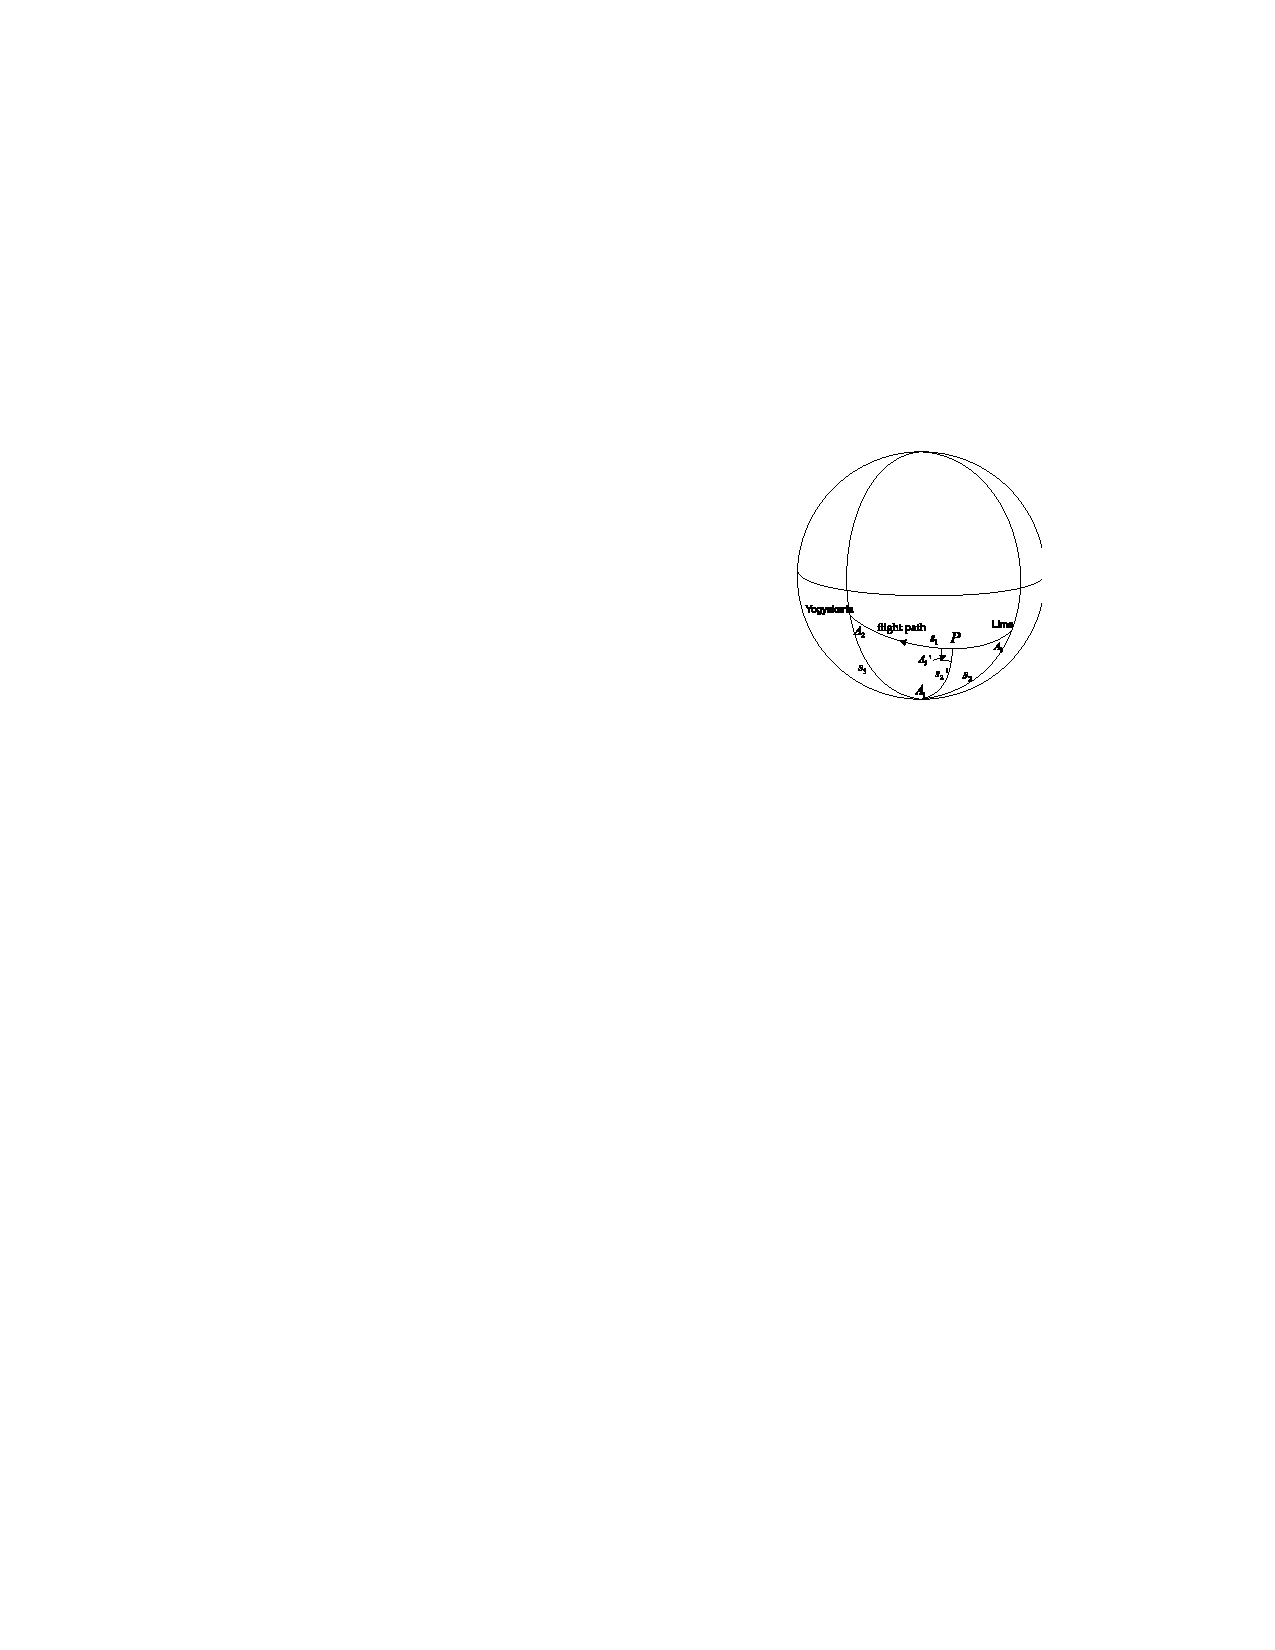
\includegraphics[pagebox=mediabox,viewport=376 455 504 576,clip,
      width=0.75\linewidth]{2015_TH_S15-s3.pdf}
  \end{center}
\end{description}

\solhead{1.21}{Shadows}
% source id: 2016_TH_T4
As the longest shadow of the Sun on the given day is of finite length, the
Sun is circumpolar for this observer on this day. \hfill[2.0]

\ioaafig{2016_TH_T4-s1.pdf}
In the figure, the left panel shows the shadow $OS$ formed by stick $OA$ (of
length 1.000\,m), and the right panel shows the Sun's location in two cases.

For an altitude $\theta$ of the Sun,
\[ \tan\theta = \frac{OA}{OS} = \frac{1.000\ \mathrm{m}}{OS} \]
\[ \therefore\ \cot\theta = OS\ \text{(in metres)} \]
\hfill[1.0]

Let $\theta_1$ and $\theta_2$ be the altitude in the two extreme cases.
\[ \theta_1 = 180^\circ - \phi - (90^\circ - \delta_\odot)
   = 90^\circ - \phi + \delta_\odot \]
\hfill[1.0]
\begin{align*}
\cot(90^\circ - \phi + \delta_\odot) &= 1.732\\
\therefore\ \tan(\phi - \delta_\odot) &= 1.732\\
\phi - \delta_\odot &= \tan^{-1}(1.732) = 60^\circ = 1.047\ \mathrm{rad}
\end{align*}
\hfill[1.5]
\[ \theta_2 = \phi - (90^\circ - \delta_\odot)
   = \phi - 90^\circ + \delta_\odot \]
\hfill[1.0]
\begin{align*}
\cot(\phi - 90^\circ + \delta_\odot) &= 5.671\\
\therefore\ \tan(\phi - 90^\circ + \delta_\odot) &= \frac{1}{5.671}\\
\phi + \delta_\odot &= \tan^{-1}\left(\frac{1}{5.671}\right) + 90^\circ
  = 100^\circ = 1.745\ \mathrm{rad}
\end{align*}
\hfill[1.5]

Solving,
\[ \boxed{\phi = 80^\circ} = 1.396\ \mathrm{rad} \]
\hfill[1.0]
\[ \boxed{\delta_\odot = 20^\circ} = 0.349\ \mathrm{rad} \]
\hfill[1.0]

Given high accuracy of shadow length, only $\pm 0.5^\circ$ is allowed.

One can also solve the question by manipulating $\tan(\phi - \delta_\odot)$
and $\tan(\phi + \delta_\odot)$, to get $\tan(\phi)$ and $\tan(\delta_\odot)$.

\solhead{1.22}{The Large Magellanic Cloud in Phuket}
% source id: 2017_TH_T1
\ioaafig{2017_TH_T1-s1.pdf}
When it culminates, $\mathrm{LHA} = 0$,
$\mathrm{RA} = -\mathrm{LST}$ \hfill[1.0]
\begin{align*}
\mathrm{LST} &= -(\mathrm{L} - \mathrm{GST}^{*}) = -\mathrm{RA}\\
\mathrm{GST}^{*} &= \mathrm{L} - \mathrm{RA}
  = 6^{\mathrm{h}}\,34^{\mathrm{min}} - 5^{\mathrm{h}}\,24^{\mathrm{min}}
  = 1^{\mathrm{h}}\,10^{\mathrm{min}}
\end{align*}
\hfill[2.0]
\begin{align*}
\mathrm{GST} &= 24^{\mathrm{h}} - 1^{\mathrm{h}}\,10^{\mathrm{min}}\\
\mathrm{GST} &= 22^{\mathrm{h}}\,50^{\mathrm{min}}
\end{align*}
\hfill[1.0]

Phuket time of 21:00 is UT\,14:00. \hfill[1.0]

\[ \mathrm{GST} = \text{GST of 1st Jan}
   + \text{The angle that $\Upsilon$ moves away from 1st Jan}
   + \mathrm{UT} \]
\hfill[1.0]
\begin{align*}
22^{\mathrm{h}}\,50^{\mathrm{min}}
  &= 6^{\mathrm{h}}\,43^{\mathrm{min}}
   + \left[\left(\frac{\text{Days that away from 1st Jan}}
                     {365.2422\ \text{days}}\right)\times 24\ \mathrm{h}\right]
   + \left[14^{\mathrm{h}}\times\left(\frac{24}{23.9344}\right)\right]\\
\text{Days that away from 1st Jan}
  &= (22^{\mathrm{h}}\,50^{\mathrm{min}} - 6^{\mathrm{h}}\,43^{\mathrm{min}}
    - 14^{\mathrm{h}}\,2^{\mathrm{min}})
    \left(\frac{365.2422\ \text{days}}{24^{\mathrm{h}}}\right)
\end{align*}
\hfill[2.0]

Days that away from 1st Jan $= 31.7$ days from 1st Jan (at Greenwich).
\hfill[1.0]

The time of the year that the LMC culminates in Phuket is on 2nd February.
\hfill[1.0]

\solhead{1.23}{Shipwreck}
% source id: 2017_TH_T12
\begin{description}
\item[a)] Draw a correct celestial sphere. \hfill[4.0]
  \ioaafig{2017_TH_T12-s1.pdf}
  \[ \frac{\sin\mathrm{LHA}^{*}}{\sin z}
     = \frac{\sin\mathrm{A}}{\sin(90^\circ - \delta)} \]
  \hfill[2.0]
  \begin{align*}
  \mathrm{LHA}^{*} &= \sin^{-1}\left(
    \frac{\sin\mathrm{A}\,\sin z}{\sin(90^\circ - \delta)}\right)\\
  &= \sin^{-1}\left(
    \frac{\sin 109^\circ\,\sin 37.5^\circ}{\sin 98.18^\circ}\right)
  \end{align*}
  \hfill[2.0]
  \[ \mathrm{LHA}^{*} = 35.56^\circ = 2^{\mathrm{h}}\,22\ \mathrm{min} \]
  \[ \mathrm{LHA} = 24^{\mathrm{h}} - 2^{\mathrm{h}}\,22\ \mathrm{min}
     = 21^{\mathrm{h}}\,38\ \mathrm{min} \]
  \hfill[2.0]

\item[b)] Bangkok time of 01:00 21st November is Universal Time (UT) 18:00
  20th November.

  Day number $+$ Time $= 323$ day 18\,h \hfill[1.0]

  GST $=$ GST of 1st Jan $+$ The angle that $\Upsilon$ moves away from 1st
  Jan \hfill[2.0]
  \[ \mathrm{GST} = 6^{\mathrm{h}}\,43^{\mathrm{min}}
     + \left(323\tfrac{18}{24}\ \mathrm{days}\right)
       \left(\frac{1}{365.2422}\right)\times 24\ \frac{\mathrm{h}}{\mathrm{day}}
     + \left[18\mathrm{h}\times\left(\frac{24}{23.9344}\right)\right] \]
  \hfill[5.0]
  \begin{align*}
  \mathrm{GST} &= 6^{\mathrm{h}}\,43^{\mathrm{min}}
    + 21^{\mathrm{h}}\,16\ \mathrm{min} + 18^{\mathrm{h}}\,3^{\mathrm{min}}\\
  \mathrm{GST} &= 46^{\mathrm{h}}\,2^{\mathrm{min}}\\
  \mathrm{GST} &= 21^{\mathrm{h}}\,58^{\mathrm{min}}
  \end{align*}
  \hfill[2.0]

  Any other correct alternative methods that provide the correct answer are
  also acceptable.

\item[c)]
  \ioaafig{2017_TH_T12-s2.pdf}
  \begin{align*}
  24^{\mathrm{h}} - \mathrm{LHA} &= \mathrm{RA} - \mathrm{LST}\\
  \mathrm{LST} &= \mathrm{RA} - 24^{\mathrm{h}} + \mathrm{LHA}\\
  \mathrm{L} &= \mathrm{RA} + \mathrm{LHA} - \mathrm{GST}\\
  \mathrm{L} &= 5^{\mathrm{h}}\,15^{\mathrm{min}}
    + 21^{\mathrm{h}}\,38\ \mathrm{min} - 21^{\mathrm{h}}\,58^{\mathrm{min}}
    = 4^{\mathrm{h}}\,55^{\mathrm{min}}
  \end{align*}
  \hfill[3.0]
  \[ \mathrm{L} = 73.75^\circ\,\mathrm{E} \]
  \hfill[2.0]

\item[d)]
  \begin{align*}
  \cos(90^\circ - \delta) &= \cos z\cos(90^\circ - \phi)
    + \sin z\sin(90^\circ - \phi)\cos\mathrm{A}\\
  \sin\delta &= \sin(h)\sin\phi + \cos(h)\cos\mathrm{A}\cos\phi
  \end{align*}
  \hfill[5.0]
  \[ \alpha = \sin\delta,\quad \beta = \sin(h),\quad
     \gamma = \cos(h)\cos\mathrm{A},\quad x = \sin\phi \]
  \[ \alpha = \beta x + \gamma\sqrt{1 - x^2} \]
  \[ (\beta^2 + \gamma^2)x^2 - 2\alpha\beta x + (\alpha^2 - \gamma^2) = 0 \]
  \hfill[1.0]
  \[ x = \frac{\alpha\beta \pm \gamma\sqrt{\gamma^2 + \beta^2 - \alpha^2}}
              {\beta^2 + \gamma^2} \]
  \hfill[1.0]
  \[ \sin\phi = \frac{\sin\delta\sin(h)
      \pm \cos(h)\cos\mathrm{A}
      \sqrt{(\cos(h)\cos\mathrm{A})^2 + \sin^2(h) - \sin^2\delta}}
     {\sin^2(h) + (\cos(h)\cos\mathrm{A})^2} \]
  \hfill[1.0]
  \[ \phi = -24.05^\circ,\ 4.01^\circ \]
  \hfill[2.0]

  For $\phi = -24.05^\circ\ \rightarrow\ \mathrm{A} = 71.0^\circ$
  \hfill[2.0]

  For $\phi = 4.01^\circ\ \rightarrow\ \mathrm{A} = 109^\circ$
  \hfill[2.0]

  The Latitude of the island is $4^\circ 1'$\,N. \hfill[1.0]
\end{description}

\textbf{Alternative Solutions}

\begin{description}
\item[b)] $-$LMT (Local Mean Time) $\rightarrow$ UT \hfill[1.0]

  Calculate the sidereal day using the given tropical year:
  \[ \gamma = \frac{\text{Sidereal time}}{\text{Solar time}}
     = \frac{24^{\mathrm{h}}\times\left(1
       + \dfrac{1}{T_{\mathrm{tropic}}}\right)}{24^{\mathrm{h}}}
     = 1 + \frac{1}{T_{\mathrm{tropic}}} = 1.002737909 \]
  \hfill[3.0]

  On the 21st November 2017, GST can be calculated from GST on 1st January
  2017.

  Day number $+$ Time $= 323$\,d 18\,h \hfill[2.0]
  \[ \mathrm{GST} = \mathrm{GST}_0 + \Delta\theta
     = \mathrm{GST}_0 + \gamma\cdot\Delta\mathrm{T} \]
  \hfill[2.0]
  \begin{align*}
  \Delta\theta &= \left(323^{\mathrm{d}}\ \tfrac{18}{24}\right)
    \cdot 1.002737909\\
  &= 324^{\mathrm{d}}.6363981
   = 15^{\mathrm{h}}16^{\mathrm{m}}24^{\mathrm{s}}.8\\
  \mathrm{GST} &= \mathrm{GST}_0
    + 15^{\mathrm{h}}16^{\mathrm{m}}24^{\mathrm{s}}.8\\
  &= 6^{\mathrm{h}}43^{\mathrm{m}}
   + 15^{\mathrm{h}}16^{\mathrm{m}}24^{\mathrm{s}}.8\\
  &= 21^{\mathrm{h}}59^{\mathrm{m}}24^{\mathrm{s}}.8
  \end{align*}
  \hfill[2.0]

\item[d)] From Cosine law:
  \begin{align*}
  \sin\delta &= (\cos z)\cdot\sin\phi + (\sin z\cos A)\cdot\cos\phi\\
  \cos z &= (\sin\delta)\cdot\sin\phi
    + (\cos\delta\cos\mathrm{LHA}^{*})\cdot\cos\phi
  \end{align*}
  \hfill[5.0]

  Correct calculation steps that can lead to the final answers. \hfill[5.0]

  Final answers:
  \[ \sin\phi = 0.0698,\quad \phi = 4.00^\circ \]
  OR
  \[ \cos\phi = 0.9976,\quad \phi = 4.00^\circ \]
  \hfill[5.0]
\end{description}

\textbf{Alternative vector solution for parts a) and d) (editorial)}

Both spherical-trigonometry steps of the official solution collapse into
single dot products if the star is written as a unit vector in the
observer's horizontal frame. Use the right-handed basis
$\{\hat{N}, \hat{E}, \hat{Z}\}$ (north, east, zenith). A star at altitude
$h$ and azimuth $A$ (measured from north through east) is the unit vector
\[ \hat{n} = (\cos h\cos A,\ \cos h\sin A,\ \sin h)
   = (-0.1982,\ 0.5756,\ 0.7934). \]
The celestial pole stands at altitude $\phi$ due north, and the celestial
equator crosses the meridian due south, so in the same basis
\[ \hat{P} = (\cos\phi,\ 0,\ \sin\phi), \qquad
   \hat{Q} = (-\sin\phi,\ 0,\ \cos\phi). \]
Projecting $\hat{n}$ onto the equatorial triad
$\{\hat{Q},\, -\hat{E},\, \hat{P}\}$ (hour angle $H$ increasing westward)
gives the star's equatorial components:
\[ \hat{n}\cdot\hat{P} = \sin\delta, \qquad
   \hat{n}\cdot\hat{E} = -\cos\delta\sin H, \qquad
   \hat{n}\cdot\hat{Q} = \cos\delta\cos H. \]
The east axis is shared by the two frames, so the middle relation contains
no $\phi$, while the pole relation contains no $H$: parts a) and d)
decouple, each into one scalar equation.

\begin{description}
\item[a)] From the shared east axis,
  \[ \sin H = -\frac{\cos h\sin A}{\cos\delta}
     = -\frac{\cos 52.5^\circ\,\sin 109^\circ}{\cos 8.18^\circ}
     = -0.5815, \]
  so $H = -35.56^\circ = -2^{\mathrm{h}}\,22^{\mathrm{min}}$, i.e.\
  $\mathrm{LHA} = 21^{\mathrm{h}}\,38^{\mathrm{min}}$. The sign (star east
  of the meridian, still rising) emerges automatically. The residual
  $\sin$ ambiguity ($H$ vs.\ $-180^\circ - H$) is settled by
  $\hat{n}\cdot\hat{Q} = 0.198\sin\phi + 0.793\cos\phi > 0$ for any
  latitude $\phi > -76^\circ$, forcing $\cos H > 0$ and hence
  $|H| < 90^\circ$.

\item[d)] The pole relation is the latitude equation in one line:
  \[ \sin\delta = \hat{n}\cdot\hat{P}
     = \underbrace{\cos h\cos A}_{C}\,\cos\phi
     + \underbrace{\sin h\vphantom{\cos A}}_{S}\,\sin\phi . \]
  Rather than squaring (which manufactures the spurious root
  $\phi = -24.05^\circ$ that the official solution must test against the
  azimuth and reject), read the right-hand side as a dot product in the
  meridian plane between the unit vector $(\cos\phi, \sin\phi)$ and the
  fixed vector $\vec{m} = (C, S) = (-0.1982,\ 0.7934)$:
  \[ |\vec{m}|\cos(\theta_m - \phi) = \sin\delta, \qquad
     |\vec{m}| = \sqrt{C^2 + S^2} = 0.8177, \]
  where $\theta_m = 104.03^\circ$ is the polar angle of $\vec{m}$,
  measured from $\hat{N}$ toward $\hat{Z}$
  ($\tan\theta_m = S/C$ with the quadrant fixed by the signs of $C$ and
  $S$). Then
  \[ \cos(\theta_m - \phi) = \frac{-0.1423}{0.8177} = -0.1741
     \quad\Rightarrow\quad \theta_m - \phi = \pm 100.02^\circ, \]
  giving $\phi = 4.00^\circ$ or $\phi = 204.05^\circ$ (no such latitude).
  The single admissible root is
  \[ \phi = 4^\circ 00'\ \mathrm{N}, \]
  in agreement with the official value ($\sin\phi = 0.0698$). No second
  root needs to be checked: the squaring step that created it never
  happened.
\end{description}

\solhead{1.24}{A Synchronous Satellite}
% source id: 2017_TH_T5
\ioaafig[1.0]{2017_TH_T5-s1.pdf}
Draw diagram and correctly identify the altitude. \hfill[1.0]

Identify another angle with the altitude $h$ in its expression, such as
$90^\circ - (\phi - \theta) - h$. \hfill[1.0]

Maximum altitude occurs when the satellite is at meridian. \hfill[1.0]

Intermediate steps that can lead to the calculation of $h$, such as
\[ \tan(90^\circ - (\phi - \theta) - h)
   = \frac{R\sin(\phi - \theta)}{H + R - R\cos(\phi - \theta)} \]
\hfill[3.0]

Correct expression for $h$: \hfill[2.0]
\[ h = 90^\circ - (\phi - \theta)
   - \tan^{-1}\left(\frac{R\sin(\phi - \theta)}
                        {H + R - R\cos(\phi - \theta)}\right) \]

Correct value of $h$:
\[ h = 90^\circ - (51.49^\circ - 6.69^\circ)
   - \tan^{-1}\left(\frac{\sin(51.49^\circ - 6.69^\circ)}
     {\dfrac{35.786\ \mathrm{km}}{6.38\times 10^{3}\ \mathrm{km}}
      + 1 - \cos(51.49^\circ - 6.69^\circ)}\right) \]
\[ h = 38.4^\circ \]
\hfill[2.0]

\emph{Maximum of 2.0 marks for solution with}
$h = 90.0^\circ - 51.49^\circ + 6.69^\circ = 45.2^\circ$.

\solhead{1.25}{Vega and Altair}
% source id: 2018_TH_T10
\begin{description}
\item[(a)] Assuming the positions of the two stars are: Vega:
  $(\alpha_1, \delta_1)$; Altair: $(\alpha_2, \delta_2)$
  \[ (\alpha_1, \delta_1) = (279.23538^\circ,\ 38.78547^\circ)
     \quad\text{and}\quad
     (\alpha_2, \delta_2) = (297.69875^\circ,\ 8.87036^\circ) \]
  \hfill(2 points)

  Cosine formula of the spherical geometry is given by:
  \[ \cos[a] = \cos[b]\cos[c] + \sin[b]\sin[c]\cos[A] \]
  \hfill(0.5 point)

  In our triangle, $b = (90 - \delta_1)$, $c = (90 - \delta_2)$ and
  $A = (\alpha_2 - \alpha_1)$. Then the angular distance $\beta$ between
  Vega and Altair is:
  \[ \cos[\beta] = \cos[90^\circ - \delta_1]\cos[90^\circ - \delta_2]
     + \sin[90^\circ - \delta_1]\sin[90^\circ - \delta_2]
       \cos[\alpha_2 - \alpha_1]; \]
  \hfill(3 points)
  \[ \cos[\beta] = \cos[51.21453^\circ]\cos[81.12964^\circ]
     + \sin[51.21453^\circ]\sin[81.12964^\circ]\cos[18.46337^\circ]; \]
  \hfill(1.5 points)
  \[ \beta = 34.19582^\circ \]
  \hfill(2 points)

\item[(b)] The distance of Vega is:
  $r_1 = 1/(130.23\times 10^{-3}) = 7.6787\,pc$

  The distance of Altair is:
  $r_2 = 1/(194.95\times 10^{-3}) = 5.1295\,pc$ \hfill(2 points)

  Using the Law of Cosines:
  $d^2 = r_1^{\,2} + r_2^{\,2} - 2r_1 r_2\cos[\beta]$ \hfill(2 point)

  we can obtain the distance: $d = 4.4855\,pc$ \hfill(2 points)

\item[(c)] Given the proper motions and radial velocities of the two stars,
  the directions of their movements on the celestial sphere can be
  estimated.

  For Vega:
  \begin{align*}
  \mu_{\alpha 1}\cos\delta_1 &= 200.94;\ \mu_{\delta 1} = 286.23\\
  \theta_1 &= \arctan\left[\frac{\mu_{\alpha 1}\cos\delta_1}
    {\mu_{\delta 1}}\right]\times\frac{180^\circ}{\pi} = 35.0697^\circ
  \end{align*}
  \hfill(2 points)

  For Altair:
  \begin{align*}
  \mu_{\alpha 2}\cos\delta_2 &= 536.23;\ \mu_{\delta 2} = 385.29\\
  \theta_2 &= \arctan\left[\frac{\mu_{\alpha 2}\cos\delta_2}
    {\mu_{\delta 2}}\right]\times\frac{180^\circ}{\pi} = 54.302^\circ
  \end{align*}
  \hfill(1 points)

\item[(d)] As the position angles of the proper motion of the two stars are
  different, the stars' paths will intersect. As the paths are circular on
  the celestial sphere, they will intersect in exactly \textbf{two} points.
  \hfill(2 points)

\item[(e)] Let the closer point of intersection be I with the coordinates
  $(\alpha_3, \delta_3)$.

  In triangle PVA,
  \[ PAV = \arcsin\left[\frac{\sin VPA\,\sin PV}{\sin VA}\right]
     = \arcsin\left[\frac{\sin(\alpha_1 - \alpha_2)
       \sin(90^\circ - \delta_1)}{\sin\beta}\right] = 26.055^\circ \]
  \[ PVA = \arcsin\left[\frac{\sin VPA\,\sin PA}{\sin VA}\right]
     = \arcsin\left[\frac{\sin(\alpha_1 - \alpha_2)
       \sin(90^\circ - \delta_2)}{\sin\beta}\right] = 146.196^\circ \]
  \hfill(5 points)

  Note that angle PVA is more than $90^\circ$, which will be evident from
  the diagram. \hfill(1 point)

  The motion of the stars on the celestial sphere will always be along some
  great circle. So VAI is a spherical triangle. Using the four parts formula
  for VAI
  \[ \cot VI = \frac{\cos VA\cos IVA + \sin IVA\cot VAI}{\sin VA} \]
  \[ VI = 90^\circ - \arctan\left[\frac{\cos 34.19582^\circ
     \cos(68.900^\circ) + \sin(68.900^\circ)\cot(99.643^\circ)}
     {\sin 34.19582^\circ}\right] = 76.085^\circ \]
  \hfill(5 points)

  by sine rule,
  \[ AI = \arcsin\left[\frac{\sin VI\sin IVA}{\sin VAI}\right]
     = \arcsin\left[\frac{\sin 76.085^\circ\sin 68.900^\circ}
       {\sin 99.643^\circ}\right] = 66.715^\circ \]
  \hfill(2 points counted in next part)

  Now we use triangle PVI: by cosine rule,
  \begin{align*}
  \cos[PI] &= \cos[PV]\cos[VI] + \sin[PV]\sin[VI]\cos[PVI];\\
  \cos[90^\circ - \delta_3] &= \cos[90^\circ - \delta_1]\cos[VI]
    + \sin[90^\circ - \delta_1]\sin[VI]\cos[180^\circ - \theta_1];\\
  \sin[\delta_3] &= \cos[51.215^\circ]\cos[76.085^\circ]
    + \sin[51.215^\circ]\sin[76.085^\circ]\cos[144.930^\circ];
  \end{align*}
  Thus, $\delta_3 = -27.945^\circ$ \hfill(4 points)

  Applying sine rule,
  \[ VPI = \arcsin\left[\frac{\sin PVI\sin VI}{\sin PI}\right]
     = \arcsin\left[\frac{\sin 144.930^\circ\sin 76.085^\circ}
       {\sin 117.945^\circ}\right] = 39.148^\circ \]
  Hence,
  $\alpha_3 = \alpha_1 - VPI = 279.235^\circ - 39.148^\circ = 240.087^\circ
   \approx 16^{\mathrm{h}}0^{\mathrm{m}}21^{\mathrm{s}}$ \hfill(5 points)

  Out of 5 points, 1 point is reserved for realising that the intersection
  point is in the past path.

\item[(f)] The total velocity along the great circle for Vega is
  \[ \mu_1 = \sqrt{(\mu_{\alpha 1}\cos\delta_1)^2 + \mu_{\delta 1}^{\,2}}
     = \sqrt{200.94^2 + 286.23^2} = 349.72\ \text{mas/year} \]
  \hfill(2 points)
  \[ \text{Number of years} = \frac{VI}{\mu_1}
     = \frac{76.085\times 3600}{0.34972} \approx 783200\ \text{years} \]
  It will happen in the year 781200 BCE. \hfill(2 points)

  Similarly, $\mu_2 = 660.30$ and number of years $= 363700$ years.

  It will happen in the year 3617 BCE.
  % sic: source says "3617 BCE"; 363700 years ago would be ~361700 BCE
  \hfill(2 points)

\item[(g)] After 363700 years, Vega would have traversed $35.335^\circ$
  along its path. \hfill(3 points)

  Thus, its separation from Altair will be
  $(76.085^\circ - 35.335^\circ) = 40.750^\circ$ \hfill(2 points)

\item[(h)] In earth centric Cartesian frame, coordinates of Vega (in units
  of parsec) will be:
  \begin{align*}
  x_1 &= r_1\cos\delta_1\cos(360^\circ - \alpha_1) = 0.96062\,\text{pc}\\
  y_1 &= r_1\cos\delta_1\sin(360^\circ - \alpha_1) = 5.90793\,\text{pc}\\
  z_1 &= r_1\sin\delta_1 = 4.80998\,\text{pc}
  \end{align*}
  Similarly, coordinates of Altair will be, $x_2 = 2.35579$,
  $y_2 = 4.48736$\,pc and $z_2 = 0.79097$\,pc. \hfill(6 points)

  Here, we are assuming the North as positive x-direction and pole as
  positive z-direction.

  The direction vectors for velocities in spherical coordinates are
  \[ v_1 = (-13.9, 7.33, 10.45)\quad\text{and}\quad
     v_2 = (-26.9, 19.57, 14.06) \]
  % sic: source uses radial velocity -26.9 for Altair though the problem
  % table gives -26.1; Altair's tangential components also appear to be
  % computed with Vega's distance (7.6787 pc) rather than Altair's
  \hfill(4 points)

  The same in Cartesian coordinates will be
  \begin{align*}
  v_{x1} &= v_{r1}\cos\delta_1\cos\alpha_1 - v_{\alpha 1}\sin\alpha_1
    - v_{\delta 1}\sin\delta_1\cos\alpha_1 = 4.45\\
  v_{y1} &= -v_{r1}\cos\delta_1\sin\alpha_1 - v_{\alpha 1}\cos\alpha_1
    + v_{\delta 1}\sin\delta_1\sin\alpha_1 = -18.33\\
  v_{z1} &= v_{r1}\sin\delta_1 + v_{\delta 1}\cos\delta_1 = -0.56
  \end{align*}
  Similarly, Cartesian velocity vector of Altair will be,
  $v_2 = (4.33, -33.85, 9.87)$. \hfill(8 points)

  Lastly, we evaluate the value of the determinant,
  \[ \begin{vmatrix}
     (x_1 - x_2) & (y_1 - y_2) & (z_1 - z_2)\\
     v_{x1} & v_{y1} & v_{z1}\\
     v_{x1} & v_{y1} & v_{z1}
     % sic: source labels the third row with Vega's components again;
     % the numbers below are Altair's
     \end{vmatrix}
   = \begin{vmatrix}
     -1.40 & 1.42 & 4.02\\
     4.45 & -18.33 & -0.56\\
     4.33 & -33.85 & 9.87
     \end{vmatrix} \]
  \[ = 279.82 - 65.81 - 286.48 = -72.47 \]
  As the value of the determinant is non-zero, the direction vectors of
  these two stars do not cross each other. Hence no such point can exist.
  \hfill(4 points)
\end{description}

\solhead{1.26}{Distance}
% source id: 2018_TH_T2
T F T F T \hfill(2 points each)

For parallaxes, we have a Gaussian with $\mu = 0.2$\,mas and
$\sigma = 0.05$\,mas, i.e.\ 25\% of the expectation value.

If we assume that the lowest and highest values of parallax are symmetric
w.r.t.\ the expected value (reasonable assumption if cluster has large
number of stars), then their distances would not be symmetric w.r.t.\ the
true distance.

$R_A > R$, $R_C = R$ (for statements (m) and (o), marks will be given only
if this relation is stated).

\solhead{1.27}{Atmospheric Refraction}
% source id: 2018_TH_T3
\begin{description}
\item[(a)] $r_d < r_u < r_l = r_r$ \hfill(4 points)
\item[(b)] When the upper edge of the Sun is under the horizon by $35'$, it
  will appear on the horizon earlier due to the influence of atmospheric
  refraction. With the apparent diurnal motion, i.e.
  \[ \omega = \frac{360^\circ}{23^{\mathrm{h}}56^{\mathrm{m}}4^{\mathrm{s}}}
     = \frac{21600'}{1436.0682^{\mathrm{m}}} = 15.0411\,'/m, \]
  \hfill(2 points)

  Ideally one should find the time taken by the mean sun to travel from
  $50'$ below horizon to $15'$ below true horizon.
  \[ \Delta t = \frac{(50' - 15')}{\omega\cos\varphi}
     = \frac{35'}{15.0411'\times\cos 40^\circ} = 3.04\ \mathrm{mins} \]
  \hfill(4 points)
\end{description}

\solhead{1.28}{Height of a Hill}
% source id: 2018_TH_T4
\ioaafig[1.0]{2018_TH_T4-s1.pdf}
First we should realise that the Sun doesn't set vertically. It sets at an
angle of $\theta = 90 - \varphi = 50^\circ$. Thus, the horizon depression
$x$ will be
\[ x = 15.0411' \times 4.1 \times \sin\theta
   = 1.03^\circ \sin 50^\circ = 0.787^\circ. \]
\hfill(4 points)

Let the height of the mountain be $H$. Let $C$ be the centre of the Earth,
point $T$ the hill top and point $T'$ the point on the horizon as seen from
$T$. Thus,
\[ \cos x = \left[\frac{R_\oplus}{(R_\oplus + H)}\right] \]
\[ H = \frac{R_\oplus(1 - \cos x)}{\cos x} = 602\ \mathrm{metres} \]
\hfill(3 points)

The distance of the horizon (from the base of the mountain, along the
surface of the earth) is found from the rectangular triangle $TCT'$ as
\[ D = (R_\oplus + H)\sin x \approx R_\oplus\sin x
   = 6.38\times 10^{3}\,\sin 0.787^\circ = 87.6\ \mathrm{km} \]
Alternatively,
\[ D = R_\oplus x = 6.38\times 10^{3}\times 0.787^\circ\times\pi
   \div 180^\circ = 87.6\ \mathrm{km} \]
\hfill(3 points)

\solhead{1.29}{Sidereal Time}
% source id: 2018_TH_T5
\begin{description}
\item[(1)] This can happen if the sidereal time is 00:00:00 just after the
  midnight and just before the midnight on the same day. It means that the Sun
  should be near the Autumn (September) Equinox. Approximate R.A. of the Sun is
  $18^{\mathrm{h}}$.
  % sic: the official solution says 18 h; at the September equinox the Sun's
  % R.A. is 12 h.
  \hfill(3 points)
\item[(2)] At $0^{\mathrm{h}}$, 1st January, 2018 (JD\,2458119.5), the mean
  sidereal time $\mathrm{GMST}_0$ was $6.706^{\mathrm{h}}$, i.e.
  $\mathrm{GMST}_0 = 100.59^\circ$. Since one mean solar day is longer than one
  mean sidereal day by $0.9856^\circ$ (about 4 minutes), the GMST will increase
  by $\Delta = 0.9856^\circ$ at next midnight on 2nd January, 2018. Therefore,
  we can first calculate how many days it will take for GMST to reach
  $360^\circ$, i.e.
  \[
    T = \frac{360^\circ - \mathrm{GMST}_0}{\Delta}
      = \frac{360^\circ - 100.59^\circ}{0.9856^\circ} = 263.20
  \]
  \hfill(3 points)

  i.e.\ after completion of 263 days, the GMST at midnight will be
  $359.80^\circ$.

  Thus, GMST will be 00:00:00 on the 264th day at 00:00:48 and then again at
  23:56:52 on the same day. \hfill(2 points)

  The 264th day in the calendar of 2018 is 21st September 2018.
  \hfill(2 points)
\end{description}

\solhead{1.30}{South to East to North}
% source id: 2019_TH_10
\begin{description}
\item[1.] The trivial solution of the problem is the North Pole ($N$). Starting
  from here we travel 6378\,km to the South ($\overset{\frown}{NA}$) along a meridian
  (e.g.\ Greenwich meridian), then 6378\,km to the East along a parallel
  ($\overset{\frown}{AB}$), and finally 6378\,km to the North ($\overset{\frown}{BN}$) (see
  figure~(a), where the black dashed lines are the Equator and the Greenwich
  meridian).

  For the general solution, mark the path to be taken in one direction with $s$
  and determine what it may be!

  Let us denote the longitude and latitude of the point $A$ by $\lambda_A$ and
  $\varphi_A$, and the point $B$ by $\lambda_B$ and $\varphi_B$.

  The triangle $ANB$ is a spherical one only if the points $A$ and $B$ are on
  the Equator (see figure~(b)), i.e.\ $\varphi_A = \varphi_B = 0^\circ$ and
  $s = R\pi/2$, because the arc $\overset{\frown}{AB}$ is lying along a great circle
  only in this case, otherwise it is a part of a parallel. The point $A$ and
  $B$ can be below the Equator as well (figure~(c)).

  \ioaafig[1.0]{2019_TH_10-s1.pdf}

  Next, we measure the angles in radians.

  The central angle of the arc $\overset{\frown}{NA}$ on the meridian fitting to the
  point $A$ ($O$ is the centre of the sphere):
  \[
    NOA\sphericalangle = \frac{\pi}{2} - \varphi,
    \quad\text{where } \varphi = \varphi_A = \varphi_B \tag{10.1}
  \]
  Thus the length $s$ of the arc $\overset{\frown}{NA}$:
  \[
    s = R\left(\frac{\pi}{2} - \varphi\right),
    \quad\text{where } s < R\pi \tag{10.2}
  \]
  The radius of the latitude circle fitting to the points $A$ and $B$:
  \[
    r_{AB} = R\sin\left(\frac{\pi}{2} - \varphi\right) = R\cos\varphi
    \tag{10.3}
  \]
  The central angle of the arc $\overset{\frown}{AB}$ is $\lambda_B - \lambda_A$,
  thus the length of the arc $\overset{\frown}{AB}$:
  \[
    s = r_{AB}\,(\lambda_B - \lambda_A) = R\cos\varphi\,(\lambda_B - \lambda_A)
    \tag{10.4}
  \]
  From the Eq.~(10.2) and Eq.~(10.4):
  \[
    \varphi = \frac{\pi}{2} - \frac{s}{R}
    \quad\text{and}\quad
    \lambda_B - \lambda_A = \frac{s}{R\cos\varphi} \tag{10.5}
  \]
  Substitute the expression of $\varphi$ from the first equation into the
  second equation:
  \[
    \lambda_B - \lambda_A = \frac{s}{R\cos\varphi}
      = \frac{\dfrac{s}{R}}{\cos\left(\dfrac{\pi}{2} - \dfrac{s}{R}\right)}
      = \frac{\dfrac{s}{R}}{\sin\dfrac{s}{R}} \tag{10.6}
  \]
  For a given arc length of $s$ ($s < R\pi$) the latitude $\varphi$ of the
  points $A$ and $B$, and the difference between their longitudes we can
  calculate from the following equations:
  \[
    \varphi = \frac{\pi}{2} - \frac{s}{R}
    \quad\text{and}\quad
    \lambda_B - \lambda_A = \frac{\dfrac{s}{R}}{\sin\dfrac{s}{R}} \tag{10.7}
  \]

  ***** Supplement. It is just for the sake of completeness, not necessary for
  the full marks.

  It is well known, that
  \[
    \lim_{x\to 0}\frac{\sin x}{x} = \lim_{x\to 0}\frac{x}{\sin x} = 1,
    \tag{10.8}
  \]
  thus $\lambda_B - \lambda_A = 1$ in case of $s \to 0$.

  Therefore the difference in longitude has a lower limit (1), but it has no
  upper limit. This means, that the distance between the points $A$ and $B$
  will increase by increasing $s$, the difference between their longitudes will
  approximate $2\pi$ (see figure~(d)), and in case of
  $\lambda_B - \lambda_A = 2\pi$ the points $A$ and $B$ will be the same (see
  figure~(e)). With further increasing of $s$ the difference
  $\lambda_B - \lambda_A$ will be larger than $2\pi$ (see figure~(f)), thus we
  have to stop at that point on the circle where the length of the path along
  it reaches the value of $s$, and then turn to the North.

  \ioaafig{2019_TH_10-s2.pdf}

  The arc length $s_{\lim}$ corresponding to the ``limit case'' of
  $\lambda_B - \lambda_A = 2\pi$ we can derive from the numerical solution of
  the following transcendent equation:
  \[
    \frac{s_{\lim}}{R} - 2\pi\sin\frac{s_{\lim}}{R} = 0
  \]
  Thus find the root of the function
  \[
    f(s) = \frac{s}{R} - 2\pi\sin\frac{s}{R},
  \]
  i.e.\ the value $s_{\lim}$, where $f(s_{\lim}) = 0$. We can solve it by
  iteration using e.g.\ the Newton--Raphson method:
  \[
    s_{k+1} = s_k - \frac{f(s_k)}{f'(s_k)}, \qquad k = 0, 1, 2, \ldots
  \]
  The first derivative of the function $f(s)$:
  \[
    f'(s) = \frac{1}{R} - \frac{2\pi}{R}\cos\frac{s}{R}
  \]
  We know that the parallel in question runs south from the Equator, thus a
  good initial value for the iteration could be $s_0 = R\pi/2 + \Delta s$,
  where $\Delta s = 1000$\,km.

  The result of the iteration and the corresponding latitude with three decimal
  places:
  \[
    s_{\lim} = 17\,206.566\ \mathrm{km}, \quad
    \varphi_{\lim} = -64.573^\circ
  \]
  $\lambda_B - \lambda_A$ is strictly increasing function of $s$ and
  \[
    \lim_{s/R\to 0} \lambda_B - \lambda_A = 1, \quad
    \lim_{s/R\to \pi} \lambda_B - \lambda_A = \infty, \tag{10.9}
  \]
  thus for any values of $0 < s < R\pi$ can be found an appropriate angle
  $\lambda_B - \lambda_A$.

  \ioaafig{2019_TH_10-s3.pdf}

  ***** End of supplement.

  In conclusion, the solution in this case is the North Pole ($N$).
  \hfill(2\,p)

  For the value of $s = 6378$\,km the solution is an (a)-type curve. The
  coordinates of the turning points are:
  \[
    \lambda_A = 0^\circ, \quad \lambda_B = 68.09^\circ, \quad
    \varphi_A = \varphi_B = 32.704^\circ
  \]
  \hfill(3\,p)

\item[2.] The non-trivial solutions are similar to the (e)-type (``lasso'')
  solution of the previous part, only the starting point is not the North Pole,
  but its location depends on the given value of arc length $s$. The circle of
  the lasso will run south from the (e)-type ``limit circle'', because the
  circumference of parallels running north from it are greater than the
  north--south arc.

  The procedure is the following.

  Knowing $s$, we have to find the parallel around the South Pole ($S$), whose
  circumference is an integer multiple of $s$. \hfill(2\,p)

  If the corresponding latitude is $\varphi_D$, then:
  \[
    2k\pi R\cos\varphi_D = s, \quad k = 1, 2, 3, \ldots \tag{10.10}
  \]
  \hfill(5\,p)

  If the latitude of the sought starting point $C$ is $\varphi_C$, then the
  length $s$ of the arc to be taken along the meridian:
  \[
    s = R\,(\varphi_C - \varphi_D) \tag{10.11}
  \]
  From the Eqs.~(10.10) and (10.11):
  \[
    \varphi_C = \varphi_D + 2k\pi\cos\varphi_D, \quad k = 1, 2, 3, \ldots
    \tag{10.12}
  \]
  Thus:
  \[
    \varphi_D = -\arccos\frac{s}{2k\pi R}, \quad k = 1, 2, 3, \ldots
    \tag{10.13}
  \]
  \hfill(2\,p)

  and
  \[
    \varphi_C = -\arccos\frac{s}{2k\pi R} + \frac{s}{R},
    \quad k = 1, 2, 3, \ldots \tag{10.14}
  \]
  \hfill(2\,p)

  The negative sign denotes that the parallel is in the southern hemisphere.

  So if the starting point is not the North Pole ($N$), there are infinitely
  many solutions.

  For the value of $s = 6378$\,km the first 5 ($k = 1, \ldots, 5$) value for
  $\varphi_D$ in degrees with 3 decimal places:
  \[
    \varphi_{D_1} = -80.842^\circ,\ \varphi_{D_2} = -85.436^\circ,\
    \varphi_{D_3} = -86.959^\circ,\ \varphi_{D_4} = -87.72^\circ,\
    \varphi_{D_5} = -88.176^\circ
  \]
  \hfill(2\,p)

  The first 5 ($k = 1, \ldots, 5$) value for $\varphi_C$ in degrees with 3
  decimal places:
  \[
    \varphi_{C_1} = -23.546^\circ,\ \varphi_{C_2} = -28.14^\circ,\
    \varphi_{C_3} = -29.663^\circ,\ \varphi_{C_4} = -30.424^\circ,\
    \varphi_{C_5} = -30.88^\circ
  \]
  \hfill(2\,p)

  In conclusion, starting to the South from a point of the parallel marked with
  a dashed red line ($C$), we get to a point on a parallel marked with a
  continuous red line ($D$). On this parallel we travel a full circle to the
  East, then we get back to the point $D$, then turn to North and travel back
  to starting point $C$.

  For the further values of $k$ the procedure is very similar, but we have to
  perform two full circles along the continuous green parallel, three along the
  blue, four along the gold, five along the brown and so on.

  Such kind of solution exists for any values of $0 < s < s_{\lim}$.

  \ioaafig{2019_TH_10-s4.pdf}
\end{description}

\solhead{1.31}{Distance to a Near-Earth Asteroid}
% source id: 2019_TH_12
\begin{description}
\item[a)] The geometric situation is the following: \hfill(5\,p)

  \ioaafig{2019_TH_12-s1.pdf}

\item[b)] One can recognize that the triangle $NOW$ is an isosceles triangle,
  two sides ($ON$ and $OW$) are equal to each other in length:
  \[
    ON = OW = R \tag{12.1}
  \]
  \hfill(1\,p)

  Therefore the angles $\alpha = ONW\sphericalangle = OWN\sphericalangle$. For
  the $NOW$ triangle we can write, that:
  \[
    2\alpha + \varphi_1 + \varphi_2 = 180^\circ
    \;\rightarrow\;
    \alpha = 90^\circ - \frac{\varphi_1 + \varphi_2}{2} \tag{12.2}
  \]
  \hfill(1\,p)

  Let us denote the direct -- i.e.\ measured through the body of the Earth, not
  on the surface -- distance between Nagykanizsa and Windhoek by $d$:
  $d = NW$. This distance can be obtained straightforward by the cosine theorem
  (one has to take care that the absolute values of the latitudes should be
  added inside the cosine function):
  \[
    d = \sqrt{R^2 + R^2 - 2R^2\cos(\varphi_1 + \varphi_2)}
      = R\sqrt{2\bigl(1 - \cos(\varphi_1 + \varphi_2)\bigr)} \tag{12.3}
  \]
  \hfill(2\,p)

  With numerical values:
  \[
    d = 1.133\,05\,R
  \]
  \hfill(1\,p)

  Let us use the following notations:
  \[
    x_1 = \overline{NA}, \quad x_2 = \overline{WA}, \quad p = p_1 + p_2
    \tag{12.4}
  \]
  For the $NOWA$ quadrilateral we can write that:
  \[
    \varphi_1 + \varphi_2 + (180^\circ - z_1) + p + (180^\circ - z_2)
      = 360^\circ \tag{12.5}
  \]
  \hfill(1\,p)

  and therefore:
  \[
    p = z_1 + z_2 - (\varphi_1 + \varphi_2) \tag{12.6}
  \]
  \hfill(1\,p)

  For the $NWA$ triangle we can write that:
  \[
    \frac{x_1}{d} = \frac{\sin(180^\circ - z_2 - \alpha)}{\sin p}
    \quad\text{and}\quad
    \frac{x_2}{d} = \frac{\sin(180^\circ - z_1 - \alpha)}{\sin p} \tag{12.7}
  \]
  \hfill(2\,p)

  Thus:
  \[
    x_1 = d\,\frac{\sin(z_2 + \alpha)}
                  {\sin(z_1 + z_2 - (\varphi_1 + \varphi_2))}
    \quad\text{and}\quad
    x_2 = d\,\frac{\sin(z_1 + \alpha)}
                  {\sin(z_1 + z_2 - (\varphi_1 + \varphi_2))} \tag{12.8}
  \]
  \hfill(2\,p)

  $D$ can be obtained either from the triangle $NOA$ or $WOA$ by the cosine
  theorem:
  \[
    D^2 = R^2 + x_1^2 - 2Rx_1\cos(180^\circ - z_1) \tag{12.9}
  \]
  or
  \[
    D^2 = R^2 + x_2^2 - 2Rx_2\cos(180^\circ - z_2) \tag{12.10}
  \]
  \hfill(2\,p)

  Let us take the sum of them:
  \[
    2D^2 = 2R^2 + (x_1^2 + x_2^2) + 2R(x_1\cos z_1 + x_2\cos z_2),
    \tag{12.11}
  \]
  \hfill(1\,p)

  where we have used that $\cos(180^\circ - x) = -\cos x$.

  (If someone determines $D$ only from one of the two ($NOA$, $WOA$)
  triangles, 1 point can be deducted, because that means, we ignore the error
  bars of one of the measurements in a significant way.)

  After substitution and dividing by two one gets:
  \[
    D^2 = R^2
      + d^2\,\frac{\sin^2(z_1 + \alpha) + \sin^2(z_2 + \alpha)}
                  {2\sin^2(z_1 + z_2 - (\varphi_1 + \varphi_2))}
      + Rd\,\frac{\sin(z_2 + \alpha)\cos z_1 + \sin(z_1 + \alpha)\cos z_2}
                 {\sin(z_1 + z_2 - (\varphi_1 + \varphi_2))} \tag{12.12}
  \]
  \hfill(3\,p)

  This contains only known quantities. After substitution we get (notice that
  for alpha and $D$ we need the absolute values of the geographical latitudes):
  \[
    \alpha = 55.5^\circ
  \]
  \hfill(1\,p)
  \[
    D = 65.8\,R = 1.1\,d_{\mathrm{Moon}}
  \]
  \hfill(2\,p)

  So, the asteroid is at 65.8 Earth-radii from the centre of the Earth. This is
  slightly more than the distance to the Moon.
\end{description}

\solhead{1.32}{The height of the chimney of Tiszaujvaros power plant}
% source id: 2019_TH_6
\begin{description}
\item[a)] (B) the one on December 16 \hfill(1\,p)

  At a given moment of the day, the Sun elevation is lower in winter on the
  northern hemisphere.

\item[b)] (B) late in the morning \hfill(1\,p)

  The shadows point slightly west of north. In fact these satellite images are
  taken at around 9:45 UTC (10:45 Central European Time).

\item[c)] The measured shadow lengths are $x_1 = 125$\,m (epoch 1, summer
  solstice) and $x_2 = 780$\,m (epoch 2, winter solstice).

  Let the unknown height of the chimney be $h$. The chimney and its shadow form
  the legs of a right-angled triangle and thus
  \begin{align*}
    \tan\alpha_1 &= h/x_1 \tag{6.1}\\
    \tan\alpha_2 &= h/x_2, \tag{6.2}
  \end{align*}
  \hfill(1\,p)

  where $\alpha_1$ and $\alpha_2$ are the Sun elevation angles at epoch 1 and
  epoch 2, respectively. \hfill(1\,p)

  At the time of the summer and winter solstices, the Earth is located at
  opposite sides of the Sun during its orbital revolution. Since the Equator is
  tilted by $\varepsilon \approx 23.5^\circ$ to the orbital plane, at a given
  point of the surface, and at a given time of the day, the Sun elevation
  angles will differ by $\alpha_1 - \alpha_2 = 2\varepsilon$ (here we ignore
  refraction and that the satellite images were not taken on the exact solstice
  days). \hfill(4\,p)

  Notice that, to a good approximation, $\alpha_1 - \alpha_2 \approx 45^\circ$.
  Assuming $\alpha_1 = \alpha_2 + 45^\circ$ makes the solution a lot easier.
  Using the trigonometric identity
  \[
    \tan\alpha_1 = \tan(\alpha_2 + 45^\circ)
      = \frac{\tan\alpha_2 + \tan 45^\circ}{1 - \tan\alpha_2 \tan 45^\circ},
    \tag{6.3}
  \]
  and substituting $\tan 45^\circ = 1$, Eq.~(6.3) becomes
  \[
    \tan\alpha_1 = \frac{1 + \tan\alpha_2}{1 - \tan\alpha_2}. \tag{6.4}
  \]
  \hfill(4\,p)

  Substituting $\tan\alpha_1$ and $\tan\alpha_2$ from Eqs.~(6.1) and (6.2) into
  Eq.~(6.4), one gets a quadratic equation for the unknown $h$:
  \[
    \frac{h}{x_1} = \frac{1 + \dfrac{h}{x_2}}{1 - \dfrac{h}{x_2}}. \tag{6.5}
  \]
  \hfill(2\,p)

  Reducing this equation to the standard format
  \[
    h^2 + h(x_1 - x_2) + x_1 x_2 = 0, \tag{6.6}
  \]
  and according to the quadratic formula, the two roots are obtained as
  \[
    h_{1,2} = \frac{x_2 - x_1 \pm \sqrt{(x_1 - x_2)^2 - 4x_1x_2}}{2}. \tag{6.7}
  \]
  \hfill(1\,p)

  Now with the measured values of $x_1 = 125$\,m and $x_2 = 780$\,m, the two
  roots for $h$ are $h_1 = 426$\,m and $h_2 = 229$\,m. \hfill(1\,p)

  Obviously, only one of the solutions is valid for our case.

  One may simply notice that $h_1 \approx 426$\,m seems just too high for a
  chimney (would in fact be comparable to the Empire State Building in New
  York, with 443\,m; the Eiffel tower in Paris is only 324\,m high).

  Alternatively, substituting $h_1 = 426$\,m into Eq.~(6.2), we obtain the Sun
  elevation angle at around the winter solstice,
  $\alpha_2 = \arctan(h_1/x_2) \approx 28.7^\circ$. However, at the geographic
  latitudes of Hungary, the Sun does not rise above ${\approx}19^\circ$ at this
  time of the year, so the larger value obtained for $h$ is clearly invalid.
  \hfill(2\,p)

  Note that according to the official data, the Tiszaújváros power plant has a
  chimney as high as $h = 250$\,m.

\item[d)] (B) and (E) \hfill(2\,p)
\end{description}

\solhead{1.33}{Radiant of a Meteor Shower}
% source id: 2020_TH_7
\begin{description}
\item[(a)] Step 1: Determine the GST at the time of observation.

  Let us denote the GST at 00:00 UT on 1st January 2020 as
  $\mathrm{GST}_0$. Total 268 days have elapsed since start of the year till
  $0^{\mathrm{h}}$ UT on 25 September. \hfill(1.0)

  At 21:00 for GMT+8 timezone, UT will be
  $21^{\mathrm{h}} - 8^{\mathrm{h}} = 13^{\mathrm{h}}$. Hence,
  \begin{align*}
    GST &= GST_0 + \Delta t\\
        &= 6^{\mathrm{h}}40^{\mathrm{m}}30^{\mathrm{s}}
           + \frac{268 \times 24}{365.2422} + \frac{13 \times 24}{23.9344}\\
        &\approx 6^{\mathrm{h}}40^{\mathrm{m}}30^{\mathrm{s}}
           + 17^{\mathrm{h}}36^{\mathrm{m}}36^{\mathrm{s}}
           + 13^{\mathrm{h}}2^{\mathrm{m}}8^{\mathrm{s}}\\
        &= 37^{\mathrm{h}}19^{\mathrm{m}}14^{\mathrm{s}}
         = \mathbf{13^{h}19^{m}14^{s}}
  \end{align*}
  \hfill(3.0)

  As longitude of observer is $120.4^\circ$, the LST of observation is,
  \begin{align*}
    LST &= GST + 24^{\mathrm{h}} \times \frac{120.4^\circ}{360^\circ}\\
        &= 13^{\mathrm{h}}19^{\mathrm{m}}14^{\mathrm{s}}
           + 8^{\mathrm{h}}1^{\mathrm{m}}36^{\mathrm{s}}\\
        &= \mathbf{21^{h}20^{m}50^{s}}
  \end{align*}
  \hfill(2.0)

\item[(b)] For horizontal coordinates

  \ioaafig{2020_TH_7-s1.pdf}
  \hfill(1.0)

  The spherical triangle has the radiant, initial position and final position
  of the $i$-th meteor to be $(A, a), (A_i, a_i)$ and $(A'_i, a'_i)$, where $a$
  and $A$ denotes the altitude and azimuth respectively.

  Using the four-parts (cotangent) equation on the left and right triangles, we
  have, for both meteors:
  \begin{align*}
    \cos(90 - a_i)\cos(A'_i - A_i)
      &= \sin(90 - a_i)\cot(90 - a'_i) - \sin(A'_i - A_i)\cot\theta\\
    \therefore \sin a_i \cos(A'_i - A_i)
      &= \cos a_i \tan a'_i - \sin(A'_i - A_i)\cot\theta
  \end{align*}
  Similarly,
  \begin{align*}
    \cos(90 - a_i)\cos(A_i - A)
      &= \sin(90 - a_i)\cot(90 - a) - \sin(A_i - A)\cot(180 - \theta)\\
    \therefore \sin a_i \cos(A_i - A)
      &= \cos a_i \tan a + \sin(A_i - A)\cot\theta
  \end{align*}
  \hfill(2.0)

  We can then eliminate $\cot\theta$ to yield:
  \[
    \frac{\sin a_i \cos(A_i - A)}{\sin(A_i - A)}
      - \frac{\cos a_i \tan a}{\sin(A_i - A)}
    = \frac{\cos a_i \tan a'_i}{\sin(A'_i - A_i)}
      - \frac{\sin a_i \cos(A'_i - A_i)}{\sin(A'_i - A_i)}
    = \cot\theta
  \]
  multiplying the whole equation by
  $\dfrac{\sin(A'_i - A_i)\sin(A_i - A)}{\cos a_i}$
  \begin{align*}
    \tan a_i \cos(A_i - A)\sin(A'_i - A)
      - \tan a \sin(A'_i - A)
      % sic: the printed solution has sin(A'_i - A) in the two left-hand
      % terms; mathematically it should be sin(A'_i - A_i).
      &= \tan a'_i \sin(A_i - A)
       - \tan a_i \cos(A'_i - A_i)\sin(A_i - A)\\
    \tan a_i \sin[(A'_i - A_i) + (A_i - A)]
      &= \tan a'_i \sin(A_i - A) + \tan a \sin(A'_i - A_i)\\
    \tan a_i \sin(A'_i - A)
      &= \tan a'_i \sin(A_i - A) + \tan a \sin(A'_i - A_i)
  \end{align*}
  \hfill(3.0)

  Plugging in $i = 1, 2$, and eliminating $\tan a$ by division, we have
  \[
    \frac{\tan a_1 \sin(A'_1 - A) - \tan a'_1 \sin(A_1 - A)}
         {\tan a_2 \sin(A'_2 - A) - \tan a'_2 \sin(A_2 - A)}
    = \frac{\sin(A'_1 - A_1)}{\sin(A'_2 - A_2)}
    \overset{\text{def}}{=} k
  \]
  where $k$ is the RHS defined above (which is a known value). Expanding the
  equation above and dividing by $\cos A$, gathering terms of $\tan A$, we get
  \[
    \tan A = \frac{\tan a_1 \sin A'_1 - \tan a'_1 \sin A_1
                   - k\tan a_2 \sin A'_2 + k\tan a'_2 \sin A_2}
                  {\tan a_1 \cos A'_1 - \tan a'_1 \cos A_1
                   - k\tan a_2 \cos A'_2 + k\tan a'_2 \cos A_2}
  \]
  \hfill(2.0)

  and
  \[
    \tan a = \frac{\tan a_1 \sin(A'_1 - A) - \tan a'_1 \sin(A_1 - A)}
                  {\sin(A'_1 - A_1)}
  \]

  Plugging in the respective values from the question,
  \begin{align*}
    A_1 &= 0^\circ  & a_1 &= 15^\circ\\
    A'_1 &= 90^\circ & a'_1 &= 0^\circ\\
    A_2 &= 210^\circ & a_2 &= 23.5^\circ\\
    A'_2 &= 255^\circ & a'_2 &= 75^\circ
  \end{align*}
  We get
  \begin{align*}
    k &= \frac{\sin(A'_1 - A_1)}{\sin(A'_2 - A_2)}
       = \frac{\sin 90^\circ}{\sin 15^\circ}\\
    k &= 1.414\\
    \tan a_1 \sin A'_1 &= 0.268\\
    \tan a'_1 \sin A_1 &= 0\\
    k\tan a_2 \sin A'_2 &= -0.594\\
    k\tan a'_2 \sin A_2 &= -2.639\\
    \tan a_1 \cos A'_1 &= 0\\
    \tan a'_1 \cos A_1 &= 0\\
    k\tan a_2 \cos A'_2 &= -0.159\\
    k\tan a'_2 \cos A_2 &= -4.571\\
    \therefore \tan A &= \frac{0.268 - 0 + 0.594 - 2.639}
                              {0 - 0 + 0.159 - 4.571} = 0.403\\
    \therefore A &= 21.94^\circ\\
    \text{OR } A &= 201.94^\circ
  \end{align*}
  \hfill(4.0)

  However, the student should realize that for $A = 21.94^\circ$, the radiant
  is in the path of the first meteor, which is unrealistic. Hence, it is more
  likely that the azimuth takes the second value. \hfill(1.0)

  Plugging in for the altitude, we find the coordinate of the radiant to be
  \begin{align*}
    \tan a_1 \sin(A'_1 - A) &= -0.249\\
    \tan a'_1 \sin(A_1 - A) &= 0\\
    \sin(A'_1 - A_1) &= 1\\
    \therefore \tan a &= (-0.2485 - 0)/1 = -0.2485\\
    a &= -13.96^\circ
  \end{align*}
  \hfill(2.0)

  As the meteor track origin and end points are rounded to integer degrees,
  the horizontal coordinates of the radiant will be
  \[
    (\mathbf{A}, \mathbf{a}) = (202^\circ, -14^\circ)
  \]
  \hfill(1.0)

  \textbf{Alternative solution}

  In the vector representation, let the starting and final locations of the
  meteroids be $\vec{u}_i$ and $\vec{v}_i$ respectively. For the subsequent
  calculations, the vectors are most conveniently represented in Cartesian
  coordinates. Letting the $x$-axis point east, $y$-axis north, and $z$-axis
  towards the zenith, we have
  \[
    \vec{u} = (u_x, u_y, u_z) = (\cos a \sin A, \cos a \cos A, \sin a)
    \tag{1}
  \]
  for a generic vector $\vec{u}$ with azimuth $A$ and altitude $a$. We can
  therefore compute
  \begin{align*}
    \vec{u}_1 &= (\cos 15^\circ \sin 0^\circ,
                  \cos 15^\circ \cos 0^\circ,
                  \sin 15^\circ) = (0, 0.9659, 0.2588)\,,\\
    \vec{u}_2 &= (\cos 23.5^\circ \sin 210^\circ,
                  \cos 23.5^\circ \cos 210^\circ,
                  \sin 23.5^\circ) = (-0.4585, -0.7942, 0.3988)\,,\\
    \vec{v}_1 &= (\cos 0^\circ \sin 90^\circ,
                  \cos 0^\circ \cos 90^\circ,
                  \sin 0^\circ) = (1, 0, 0)\,,\\
    \vec{v}_2 &= (\cos 75^\circ \sin 255^\circ,
                  \cos 75^\circ \cos 255^\circ,
                  \sin 75^\circ) = (-0.25, -0.0670, 0.9659)\,.
  \end{align*}
  \hfill(3.0)

  The meteors move along great arcs, and the two intersections of the great
  arcs correspond to the two possible locations of the radiant. A great arc is
  uniquely defined by its normal vector, denote it with $\vec{n}_i$. The
  normal vector is conveniently calculated through the cross product of the
  starting and final position, $\vec{n}_i = \vec{u}_i \times \vec{v}_i$. The
  cross product can be calculated via the determinant of the following matrix
  \[
    \vec{u}_i \times \vec{v}_i =
    \begin{vmatrix}
      i & j & k\\
      u_{ix} & u_{iy} & u_{iz}\\
      v_{ix} & v_{iy} & v_{iz}
    \end{vmatrix}
    = (u_{iy}v_{iz} - u_{iz}v_{iy},\,
       u_{iz}v_{ix} - u_{ix}v_{iz},\,
       u_{ix}v_{iy} - u_{iy}v_{ix}).
  \]
  \hfill(4.0)

  This yields
  \begin{align*}
    \vec{n}_1 &= (0, 0.2588, -0.9659)\,,\\
    \vec{n}_2 &= (-0.7404, 0.3432, -0.1678)\,.
  \end{align*}
  \hfill(1.0)

  Every point on the great circle $i$ is perpendicular to $\vec{n}_i$. This
  means that the intersections of the two great circles are perpendicular to
  both $\vec{n}_1$ and $\vec{n}_2$. The vector parallel to the intersections
  can therefore be calculated by the cross product of $\vec{n}_1$ and
  $\vec{n}_2$. Let the vector corresponding to the intersection be $\vec{m}$.
  Then
  \begin{align*}
    \vec{m} &= \vec{n}_1 \times \vec{n}_2 & \text{(3.0)}\\
            &= (0.3626, 0.9002, 0.2412)\,. & \text{(1.0)}
  \end{align*}

  Now all that's left is to calculate the azimuth and altitude corresponding
  to $\vec{m}$. Note that $-\vec{m}$ is also an intersection. The equations
  for the altitude and azimuth can be reverse-engineered from equation (1):
  \[
    a = \arctan\left(\frac{z}{\sqrt{x^2 + y^2}}\right), \qquad
    A = \arctan\left(\frac{x}{y}\right).
  \]
  \hfill(1.0)

  One has to take care that the arctans are signed. This gives the final
  values of the intersection points to be
  \[
    (A, a) = (22^\circ, 14^\circ)
    \quad\text{and}\quad
    (A, a) = (202^\circ, -14^\circ).
  \]
  \hfill(2.0)

  As in the first solution, the $A = 22^\circ$ solution can be eliminated due
  to it being on the path of the first meteor. This gives the final answer of
  \[
    (\mathbf{A}, \mathbf{a}) = (202^\circ, -14^\circ)
  \]
  \hfill(1.0)

\item[(c)] Now, it is easy to convert the horizontal coordinates of the
  radiant to equatorial coordinates.

  \ioaafig{2020_TH_7-s2.pdf}
  \hfill(1.0)

  Using the cosine rule:
  \begin{align*}
    \sin\delta &= \sin\phi \sin a + \cos\phi \cos a \cos A\\
      &= \sin(23.5^\circ)\sin(-13.4^\circ)
         + \cos(23.5^\circ)\cos(-13.96^\circ)\cos(201.94^\circ)\\
      % sic: the official solution writes -13.4 deg in two places here and
      % below where the altitude is a = -13.96 deg.
      &= -0.9217\\
    \therefore \delta &= -67.2^\circ
  \end{align*}
  \hfill(2.0)
  \begin{align*}
    \cos H &= \frac{\sin a - \sin\delta \sin\phi}{\cos\phi \cos\delta}\\
      &= \frac{\sin(-13.4^\circ) - \sin(-67.2^\circ)\sin(23.5^\circ)}
              {\cos(23.5^\circ)\cos(-67.2^\circ)} = 0.3551\\
    \therefore H &= 4^{\mathrm{h}}36^{\mathrm{m}}47^{\mathrm{s}}
  \end{align*}
  \hfill(1.5)

  From the relationship between the LST and the Hour Angle
  ($H = LST - \alpha$), we get the equatorial coordinates of the radiant to be
  \begin{align*}
    \alpha &= 21^{\mathrm{h}}20^{\mathrm{m}}50^{\mathrm{s}}
              - 4^{\mathrm{h}}36^{\mathrm{m}}47^{\mathrm{s}}\\
           &= 16^{\mathrm{h}}44^{\mathrm{m}}3^{\mathrm{s}}
  \end{align*}
  \hfill(1.5)

  Thus, the equatorial coordinates of the radiant are,
  \[
    (\alpha, \delta) = (16^{\mathrm{h}}44^{\mathrm{m}}, -67.2^\circ)
  \]

\item[(d)] Triangulum Australes \hfill(2.0)
\end{description}

\solhead{1.34}{IOAA Logo}
% source id: 2021_TH_Q8
\begin{description}
\item[(8.1)] Assuming $R = 6378$\,km (as per the table of constants)
  \begin{align*}
    \Delta x &= R \cdot
      \left[(4^\circ 36' 18'') - (4^\circ 35' 30'')\right]
      \cdot \frac{\pi}{180} = 1.4842\ \mathrm{km}\\
    \Delta y &= R \cdot
      \left[(74^\circ 3' 19'') - (74^\circ 3' 15'')\right]
      \cdot \frac{\pi \cdot \cos(4,35,54)}{180} = 0.1237\ \mathrm{km}\\
    \Delta z &= (3.100 - 3.296) = -0.196\ \mathrm{km}
  \end{align*}
  \hfill[2 points]
  \[
    d_{2-3} = \sqrt{(x^2 + y^2 + z^2)} = 1.502\ \mathrm{km}
  \]
  \hfill[1 point]

\item[(8.2)] Using the same method as part 8.1:
  \[
    d_{1-2} = 2.722\ \mathrm{km}
  \]
  \hfill[2 points]
  \[
    d_{1-3} = 2.580\ \mathrm{km}
  \]
  \hfill[2 points]

  Using Cosine rule for spherical triangle,
  \[
    \cos(A) = \frac{\bigl(d_{1-2}^{\;2} + d_{1-3}^{\;2}
                          - d_{2-3}^{\;2}\bigr)}
                   {2\,d_{1-2}\,d_{1-2}} = 0.841
    % sic: the official solution writes d_{1-2} twice in the denominator;
    % it should be 2 d_{1-2} d_{1-3}.
  \]
  \[
    A = 32.78^\circ
  \]
  \hfill[2 points]

\item[(8.3)] ~
  \[
    \alpha = \tan^{-1}\left(
      \frac{-\sin(\beta)\cdot\sin(\varepsilon)
            + \cos(\beta)\cdot\cos(\varepsilon)\cdot\sin(\lambda)}
           {\cos(\beta)\cdot\cos(\lambda)}\right)
  \]
  \[
    \alpha = 12^\circ 43' 3''
           = 0^{\mathrm{h}} 50^{\mathrm{m}} 52^{\mathrm{s}}
  \]
  \hfill[3 points]
  \[
    \delta = \sin^{-1}\bigl(\sin(\beta)\cdot\cos(\varepsilon)
             + \cos(\beta)\cdot\sin(\varepsilon)\cdot\sin(\lambda)\bigr)
  \]
  \[
    \delta = 1^\circ 33' 43''
  \]
  \hfill[3 points]
\end{description}

\solhead{1.35}{Georgia to Georgia}
% source id: 2022_TH_7
\ioaafig{2022_TH_7-s1.pdf}

In the diagram, $N$ is the northernmost point of the path
$\overset{\frown}{AB}$. Triangle $APB$, triangle $APN$ and triangle $BPN$ are
all spherical triangles. We shall use the convention that North and West are
positive, and South and East are negative. We notice,
\begin{align*}
  \overset{\frown}{PN} &= -\delta_F = 30^\circ 4'\\
  \overset{\frown}{PA} &= 90^\circ - \phi_A = 48^\circ 17'\\
  \overset{\frown}{PB} &= 90^\circ - \phi_B\\
  \sphericalangle PNA &= \sphericalangle PNB = 90^\circ\\
  \sphericalangle BPA &= \lambda_B - \lambda_A
\end{align*}
\hfill(5.0)
\begin{align*}
  x = \overset{\frown}{AB} &= vt = 4375 \times 2\tfrac{17}{60}
    = 9990\ \mathrm{km}\\
  \therefore x &= \frac{9900}{R_\oplus} = 1.5663\ \mathrm{rad}
  % sic: the official solution writes 9900 here; from the previous line it
  % should be 9990 km.
  \\
  &= 89.74^\circ = 89^\circ 44'
\end{align*}
\hfill(2.0)

In $\triangle APN$, using sine rule,
\begin{align*}
  \frac{\sin\sphericalangle A}{\sin\overset{\frown}{PN}}
    &= \frac{\sin\sphericalangle N}{\sin\overset{\frown}{PA}}\\
  \therefore \sin\sphericalangle A
    &= \frac{\sin 90^\circ \sin(30^\circ 4')}{\cos\phi_A}
     = \frac{\sin(30^\circ 4')}{\cos(41^\circ 43')} = 0.67119\\
  \therefore \sphericalangle A
    &= 0.7358\ \mathrm{rad} = 42.16^\circ = 42^\circ 10'
\end{align*}
\hfill(3.0)

(Recognise that to have a northern point on the path, it must be the acute
solution)

In $\triangle PBA$, using cosine rule,
\begin{align*}
  \cos\overset{\frown}{PB}
    &= \cos\overset{\frown}{PA}\cos\overset{\frown}{AB}
     + \sin\overset{\frown}{PA}\sin\overset{\frown}{AB}
       \cos\sphericalangle A\\
  \sin\phi_B &= \sin\phi_A \cos x + \cos\phi_A \sin x \cos A\\
    &= \sin(41^\circ 43')\cos(89^\circ 44')
     + \cos(41^\circ 43')\sin(89^\circ 44')\cos(42^\circ 10')\\
  \sin\phi_B &= 0.5563\\
  \therefore \phi_B &= 0.5900\ \mathrm{rad} = 33.80^\circ = 33^\circ 48'
\end{align*}
\hfill(4.0)

(Only one solution in the valid values of latitude)

Again using cosine rule,
\begin{align*}
  \cos\overset{\frown}{AB}
    &= \cos\overset{\frown}{PA}\cos\overset{\frown}{PB}
     + \sin\overset{\frown}{PA}\sin\overset{\frown}{PB}
       \cos\sphericalangle P\\
  \therefore \cos\sphericalangle P
    &= \frac{\cos x - \sin\phi_A \sin\phi_B}{\cos\phi_A \cos\phi_B}\\
    &= \frac{\cos(89^\circ 44') - \sin(41^\circ 43')\sin(33^\circ 48')}
            {\cos(41^\circ 43')\cos(33^\circ 48')}\\
  \cos\sphericalangle P &= -0.5891\\
  \therefore \sphericalangle P
    &= 2.201\ \mathrm{rad} = 126.13^\circ = 126^\circ 8'\\
  \lambda_B &= \sphericalangle P + \lambda_A = 126^\circ 8' - 41^\circ 48'\\
  \lambda_B &= 1.472\ \mathrm{rad} = 84.33^\circ = 84^\circ 20'
\end{align*}
\hfill(5.0)

(The other solution of $\lambda_B - \lambda_A = -126.13^\circ$ gives
$\lambda_B = -167.93^\circ$ which is clearly not valid)

Therefore, the coordinates of Atlanta are
\[
  (33^\circ 48'\mathrm{N}, 84^\circ 20'\mathrm{W})
\]
\hfill(1.0)

\medskip
\noindent\textbf{Alternative method to find $L_2$}

Using the spherical sine rule in triangle $PBA$,
\begin{align*}
  \frac{\sin A}{\sin(90^\circ - \phi_2)}
    &= \frac{\sin(L_2 - L_1)}{\sin x}\\
  \therefore \sin(L_2 - L_1) &= \frac{\sin x \sin A}{\cos\phi_2}\\
  \therefore \sin(L_2 - L_1)
    &= \frac{\sin(89^\circ 51')\sin(42^\circ 10')}{\cos(33^\circ 43')}
     = 0.80689\\
  \therefore L_2 - L_1
    &= 126.21^\circ \quad (= 126^\circ 12' = 2.20\ \mathrm{rad})\\
  \therefore L_2 &= 126^\circ 12' + L_1
    = 126^\circ 12' + (-41^\circ 48') = 84.41^\circ
    \quad (= 84^\circ 24' = 1.47\ \mathrm{rad})
\end{align*}

(The other solution of $L_2 - L_1 = 53.79^\circ$ gives $L_2 = 11.99^\circ$
which is clearly not valid)

Accept all other valid solutions (such as the four parts rule or using
Napier's rules) that give $\phi_2 = 33.71^\circ$ and $L_2 = 84.41^\circ$.
Students may do both methods for calculating $L_2$ to confirm which solution
is common to both as a quicker check than trying to do the reverse calculation
with a given pair of co-ordinates.

\solhead{1.36}{Neptune}
% source id: 2023_TH_Q1
Using Kepler's Third law and the semi-major axis ($a = 30.070$\,au) of the
orbit from the table of constants, the sidereal period of Neptune's orbit is:
\[
  P_{\mathrm{N}} = (a^3)^{\frac{1}{2}} = \sqrt{27189.4}
    = 164.89\ \mathrm{years} \hfill
\]
\hfill(1 point)

The rest of the calculation can be done in (at least) two ways:

\medskip
\noindent\textbf{(1) `day counting'/`date drift' solution:}

Since Neptune is an outer planet (relative to Earth), the synodic period $S$ in
years is given by:
\[
  \frac{1}{S} = \frac{1}{1\ \mathrm{year}} - \frac{1}{P_{\mathrm{N}}}
\]
\hfill(1 point)
\begin{align*}
  &= 1 - \frac{1}{164.89} = 1 - 0.006065 = 0.99394\\
  &\Longrightarrow S = 1/0.99394 = 1.006102\ \mathrm{years}
\end{align*}
\hfill(1 point)
\[
  \Longrightarrow 1.006102 \times 365.2422 = 367.4708\ \mathrm{solar\ days}
\]

Therefore the date of opposition drifts by:
\[
  D = 367.4708 - 365.2422 = 2.2286\ \mathrm{days/year}
\]
\hfill(1 point)

The approximate date of the northern spring equinox is 20 March. The number of
days between 21 September and 20 March $= 185$ days, therefore year of desired
opposition is:
\[
  2024 - (185/D) = 2024 - 83 = 1941
\]
\hfill(1 point)

If the student takes 21 March as the spring equinox, they get
$184/D = 82.5\,\mathrm{yr} \Longrightarrow 1942$.

\medskip
\noindent\textbf{(2) `angular drift' solution (more accurate)}

As before, the synodic period of Neptune can be derived as:
\[
  \frac{1}{S} = \frac{1}{1\ \mathrm{year}} - \frac{1}{P_{\mathrm{N}}}
\]
\hfill(1 point)
\[
  = 1 - \frac{1}{164.89} = \frac{163.89}{164.89}
  \Longrightarrow S = \frac{164.89}{163.89}\ \mathrm{years}
\]
Therefore the ecliptic longitude of Neptune at opposition drifts by
$(360^\circ/163.89)/\mathrm{year}$. We want to find how many years it takes for
the longitude of opposition to move by $180^\circ$, i.e.\ for what $t$:
\[
  t \times \frac{360^\circ}{163.89} = 180^\circ.
\]
\hfill(2 points)
\[
  \Longrightarrow t = 163.89/2 = 81.95\ \mathrm{years}
  \Longrightarrow 2024 - 82 = 1942
\]
\hfill(1 point)

We accept 1941 or 1942 for full points for calculations using the assumptions
in the question. If the student uses some other method which is conceptually
correct and results in 1943 (the true answer) they should also get full
points.

\medskip
Table of spring equinoxes and oppositions of Neptune:

\begin{center}
\begin{tabular}{|c|c|c|c|r|}
\hline
Year & Equinox (UT) & Opposition (UT) & Coordinates of Neptune
  & $\Delta T$ [days]\\
\hline
1940 & Mar 20 18:42 & Mar 14 21:08
  & $11^{\mathrm{h}}40^{\mathrm{m}}$ $+3^\circ 28'$ & $5.9$\\
1941 & Mar 21 00:20 & Mar 17 07:40
  & $11^{\mathrm{h}}49^{\mathrm{m}}$ $+2^\circ 39'$ & $3.7$\\
1942 & Mar 21 06:11 & Mar 19 18:12
  & $11^{\mathrm{h}}57^{\mathrm{m}}$ $+1^\circ 50'$ & $1.5$\\
1943 & Mar 21 12:03 & Mar 22 04:51
  & $12^{\mathrm{h}}04^{\mathrm{m}}$ $+1^\circ 00'$ & $-0.7$\\
1944 & Mar 20 17:49 & Mar 23 15:29
  & $12^{\mathrm{h}}13^{\mathrm{m}}$ $+0^\circ 11'$ & $-2.9$\\
\hline
2024 & Mar 20 03:06 & Sep 21 00:16
  & $23^{\mathrm{h}}55^{\mathrm{m}}$ $+1^\circ 56'$ & $-184.9$\\
\hline
\end{tabular}
\end{center}

Taking into account all effects, the last opposition closest to the spring
equinox was actually in 1943. 1942 results from the assumptions made in the
question.

\solhead{1.37}{Aldebaran}
% source id: 2023_TH_Q10
\begin{description}
\item[(a)] Aldebaran is far enough away that the light rays from it can be
  considered to be parallel, thus the problem can be modelled by the following
  diagram:

  \ioaafig{2023_TH_Q10-s1.pdf}

  where the light ray through $C$ passes through the centre of the Earth and
  thus $\delta_{\mathrm{A}}$ is the declination of Aldebaran; the ray through
  $D$ and $B$ (Bologna) represents the situation observed by Copernicus, with
  Aldebaran behind the Moon and $0.32'$ above the south edge; and the ray
  through $M$ and $P$ represents the situation where Aldebaran is exactly
  behind the centre of the Moon. $\varphi_{\mathrm{B}}$ is the geocentric
  latitude of Bologna, $\varphi_1$ is the latitude of the place $P$ and $r$ is
  the radius of the Earth (assume the Earth is spherical).

  Calculating the latitude $\varphi_1$ is thus a matter of simple geometry,
  where:
  \begin{align*}
    |CD| &= r\sin(\varphi_{\mathrm{B}} - \delta_{\mathrm{A}}),\\
    |CM| &= r\sin(\varphi_1 - \delta_{\mathrm{A}}),
  \end{align*}
  and the distance $|DM|$ is the fraction of the Moon's radius given by:
  \[
    |DM| = 1\,737\ \mathrm{km} \times
      \left(1 - \frac{0.32'}{31.5'/2}\right) = 1\,702\ \mathrm{km}.
  \]
  Therefore, since
  \begin{align*}
    |CM| &= |CD| + |DM| = 3\,099\ \mathrm{km} + 1\,702\ \mathrm{km}
          = 4\,801\ \mathrm{km},\\
    \Longrightarrow\ \varphi_1 &= \arcsin\left(\frac{4\,801}{6\,378}\right)
      + \delta_{\mathrm{A}} = 64.19^\circ.
  \end{align*}
  \hfill(6 points)

\item[(b)] Given the assumptions, the duration of the occultation will just
  depend on the difference between the tangential speeds of the observer,
  $v_{\mathrm{obs}}$, and Moon, $v_{\mathrm{Moon}}$, and on the diameter of
  the Moon.

  For the observer, the tangential speed is given by the circumference of
  their path at latitude $\varphi_1$ divided by the sidereal day:
  \[
    v_{\mathrm{obs}} = \frac{2\pi r_{\mathrm{Earth}} \cos\varphi_1}
                            {23^{\mathrm{h}}\,56\mathrm{m}\,4^{\mathrm{s}}}
                     = 729\ \mathrm{km/h}
  \]

  \ioaafig{2023_TH_Q10-s2.pdf}

  Similarly for the Moon, using the semi-major axis of the Moon's orbit and
  the length of the sidereal month (from the table of constants):
  \[
    v_{\mathrm{Moon}} = \frac{2\pi \times 3.844 \times 10^5\ \mathrm{km}}
                             {27.321661\ \mathrm{d} \times 24}
                      = 3\,683\ \mathrm{km/h}
  \]
  The difference of speeds is then:
  \[
    v_{\mathrm{rel}} = v_{\mathrm{Moon}} - v_{\mathrm{obs}}
                     = 2\,954\ \mathrm{km/h}
  \]
  and the time taken to move across the lunar diameter
  ($2 \times 1737$\,km) at that speed is:
  \[
    t = \frac{2 \times 1\,737\ \mathrm{km}}{2\,954\ \mathrm{km/h}}
      = 1.176 \approx 1.18\ \mathrm{hours}.
  \]
  \hfill(5 points)

\item[(c)] To determine the topocentric angular velocity, we need to find the
  distance $d$ between the observer (at place $P$ at latitude $\varphi_1$) and
  the Moon:

  \ioaafig{2023_TH_Q10-s3.pdf}

  where $a$ is the semi-major axis of the Moon's orbit, $\delta$ is the
  geocentric declination of the Moon, and $\delta'$ is the topocentric
  declination of the Moon as seen by the observer. We can rewrite
  $\varrho = \delta - \delta'$ and
  $\alpha = 180^\circ - (\varphi_1 - \delta) - \varrho
          = 180^\circ - (\varphi_1 - \delta) - (\delta - \delta')
          = 180^\circ - (\varphi_1 - \delta')$,
  then using the sine theorem:
  \[
    \frac{d}{\sin(\varphi_1 - \delta)}
      = \frac{a}{\sin\left(180^\circ - (\varphi_1 - \delta')\right)}
      = \frac{r}{\sin(\delta - \delta')}
  \]
  Simplifying and substituting $\delta' = \delta_{\mathrm{A}}$:
  \[
    \frac{d}{\sin(\varphi_1 - \delta)}
      = \frac{a}{\sin(\varphi_1 - \delta_{\mathrm{A}})}
      = \frac{r}{\sin(\delta - \delta_{\mathrm{A}})}
  \]
  We can now calculate $\delta$:
  \[
    \delta = \arcsin\left(
        \frac{r\sin(\varphi_1 - \delta_{\mathrm{A}})}{a}\right)
      + \delta_{\mathrm{A}} = 16.08^\circ
  \]
  and $d$:
  \[
    d = a\,\frac{\sin(\varphi_1 - \delta)}
                {\sin(\varphi_1 - \delta_{\mathrm{A}})}
      = 380\,203\ \mathrm{km}.
  \]
  Thus the angular velocity is:
  \[
    \omega = \left(\frac{2\,R_{\mathrm{Moon}}}{d}\right)
             \left(\frac{1}{1.176\ \mathrm{h}}\right) \mathrm{rad/h}
           = \left(\frac{2 \times 1\,737}{380\,203}\right)
             \left(\frac{1}{1.176\ \mathrm{h}}\right)
             \left(\frac{180 \times 60}{\pi}\right)
           = 26.71 \approx 27\ \mathrm{arcmin/h}.
  \]
  \hfill(7 points)

\item[(d)] The result in part (c), 27\,arcmin/h, was calculated for the
  situation when the Moon and observer are moving in the same direction,
  reducing their relative velocity, and thus represents the lower limit of the
  range of topocentric angular velocities. The upper limit is given by the
  situation when the Moon and observer are moving in the opposite direction,
  i.e.\ when the Moon is due north.

  Using the calculation from part (b), we find that the relative linear speed
  is:
  \[
    v'_{\mathrm{rel}} = v_{\mathrm{Moon}} + v_{\mathrm{obs}}
                      = 3\,683 + 729 = 4\,412\ \mathrm{km/h}
  \]
  Neglecting the effect of the slightly greater distance between the observer
  and the Moon when the Moon is on the northern side of the sky, the angular
  speed will be greater by the ratio of the linear speeds,
  \[
    \omega' = \omega\,\frac{4\,416}{2\,954} = 39.89
            \approx 40\ \mathrm{arcmin/h},
    % sic: the official solution writes 4416 here; the relative speed derived
    % above is 4412 km/h.
  \]
  thus the range is approximately 27--40 arcmin/h. \hfill(3 points)

  If the additional distance is taken into account, the upper limit will be
  around 1\% less.

  Expressing the velocities as vectors,
  \[
    \vec{v}_{\mathrm{rel}} = \vec{v}_{\mathrm{Moon}} - \vec{v}_{\mathrm{obs}},
  \]
  the magnitude of the relative velocity,
  $v_{\mathrm{rel}} = |\vec{v}_{\mathrm{rel}}|$ is given by the scalar
  projection of $\vec{v}_{\mathrm{obs}}$ on $\vec{v}_{\mathrm{Moon}}$:
  \[
    v_{\mathrm{rel}} = v_{\mathrm{Moon}} - v_{\mathrm{obs}}\cos\alpha
  \]
  where $\alpha$ is the angle between the vectors. From this it can be seen
  that the relative velocity must be minimum for $\alpha = 0^\circ$ and
  maximum for $\alpha = 180^\circ$. These conditions are met on the local
  meridian, due south or due north, respectively. \hfill(4 points)
\end{description}

\solhead{1.38}{Sundial}
% source id: 2024_TH_T1
\begin{description}
\item[(a)] \textbf{True}. The polar rod of the sundial faces the hemisphere
  that contains the south cardinal point as the fundamental pole, so the
  sundial was designed for a location in the southern hemisphere of the Earth.
\item[(b)] \textbf{False}. This curve represents the trajectory of the tip of
  the rod's shadow throughout the day of the summer solstice in the hemisphere
  in which the sundial is located.
\item[(c)] \textbf{True}. This straight line, which is perpendicular to the
  meridian line, represents the trajectory of the tip of the rod's shadow
  throughout the day of either southern autumnal or vernal equinox.
\item[(d)] \textbf{False}. This set of radial lines corresponds to the true
  local solar time. The 12h line coincides with north--south line, which must
  be the case for the true solar noon.
\item[(e)] \textbf{True}. The dashed lines and the solid lines form an angle
  corresponding to the longitude difference between the sundial and the center
  of the time zone. Therefore, the dashed lines correspond to the true solar
  time of the center of the time zone. An analemma shaped figure around the
  line that corresponds to a true local solar time indicates the mean solar
  time.
\end{description}

\solhead{1.39}{Castaway}
% source id: 2024_TH_T7
\begin{description}
\item[(a)] The first step is to find an expression for the azimuth of an
  object during sunrise:

  \ioaafig{2024_TH_T7-s1.pdf}

  Using the law of cosines:
  \begin{align*}
    \cos(90^\circ + \delta)
      &= \cos(90^\circ - a)\cos(90^\circ + \phi)
       + \sin(90^\circ - a)\sin(90^\circ + \phi)\cos(180^\circ - A)\\
    \therefore -\sin(\delta)
      &= -\sin(a)\cos(\phi) - \cos(a)\cos(\phi)\cos(A)
      % sic: the official solution writes -sin(a)cos(phi) for the first term;
      % expanding the law of cosines gives -sin(a)sin(phi). The term vanishes
      % anyway since a = 0 at sunrise.
  \end{align*}
  Since the altitude $a = 0^\circ$ at the sunrise:
  \[
    \cos(\phi) = \frac{\sin(\delta)}{\cos(A)}
  \]
  \hfill(2.0)

  Note that due to symmetry over the local meridian, the azimuth of sunrise
  corresponds to $180^\circ$ minus half of the angle given in the question
  statement (the $180^\circ$ term comes from the fact that the observer is on
  the southern hemisphere).

  The scenarios that lead to the minimum and maximum values of latitude
  correspond to the extreme values for the declination of the Sun in the
  southern hemisphere summer ($-23.5^\circ$ and $0^\circ$).

  If the declination of the Sun is $-23.5^\circ$, the latitude has to be
  \begin{align*}
    \cos(\phi) &= \frac{\sin(-23.5^\circ)}
                       {\cos\left(180^\circ - \frac{120^\circ}{2}\right)}\\
    \cos(\phi) &= -2\,\sin(-23.5^\circ)\\
    \phi &= -37.1^\circ
  \end{align*}
  \hfill(2.0)

  Only the negative solution of this equation is relevant in this case since
  the observer is in the southern hemisphere.

  If the declination of the Sun is $0^\circ$, simply plugging in this value to
  the formula will result in a latitude of $-90^\circ$. Since celestial
  objects do not rise or set at the poles, this approach would not be
  conceptually correct. However, at a point infinitesimally close to the pole,
  the Sun would still mathematically rise and set, and it would be possible to
  achieve the difference in azimuth from the problem statement with a
  declination very close to $0^\circ$. Thus, although a latitude of
  $-90^\circ$ is impossible, any latitude infinitesimally close to it would
  still mathematically be possible.

  Therefore, the range of possible latitudes for the island is the following:
  \[
    -90^\circ < \phi \leq -37.1^\circ
  \]
  \hfill(3.0)

\item[(b)] Since the latitude is constant, the following expression must be
  true:
  \[
    \cos(\phi) = \frac{\sin(\delta_0)}{\cos(A_0)}
               = \frac{\sin(\delta_{40})}{\cos(A_{40})}
  \]
  \hfill(2.0)

  It is also possible to apply the law of sines to the following triangle to
  derive another expression for the declination of the Sun on each day:

  \ioaafig{2024_TH_T7-s2.pdf}
  \hfill(1.0)

  \begin{align*}
    \frac{\sin(\theta_0)}{\sin(90^\circ)}
      &= \frac{\sin(-\delta_0)}{\sin(\epsilon)}\\
    \sin(\delta_0) &= -\sin(\theta_0)\sin(\epsilon)
  \end{align*}
  Analogously:
  \begin{align*}
    \frac{\sin(\theta_{40})}{\sin(90^\circ)}
      &= \frac{\sin(-\delta_{40})}{\sin(\epsilon)}\\
    \sin(\delta_{40}) &= -\sin(\theta_{40})\sin(\epsilon)
  \end{align*}
  \hfill(1.0)

  Combining the three previous expressions:
  \begin{align*}
    \sin(\delta_0) &= \frac{\sin(\delta_{40})\cos(A_0)}{\cos(A_{40})}\\
    -\sin(\theta_0)\sin(\epsilon)
      &= \frac{-\sin(\theta_{40})\sin(\epsilon)\cos(A_0)}{\cos(A_{40})}\\
    \sin(\theta_0) &= \frac{\sin(\theta_{40})\cos(A_0)}{\cos(A_{40})}\\
    \sin(\theta_0) &= k\,\sin(\theta_{40})
  \end{align*}
  \hfill(2.0)

  Where
  $k = \dfrac{\cos(A_0)}{\cos(A_{40})}
     = \dfrac{\cos(120^\circ)}{\cos(98.5^\circ)} = 3.38$.

  In order to replace one variable and solve for $\theta_0$, it is possible to
  consider that the angular velocity of the Sun on the Ecliptic is
  approximately constant due to the Earth's very low eccentricity. In that
  case, the following expression must be true:
  \begin{align*}
    \theta_{40} &= \theta_0 - \frac{40}{T_{year}} \times 360^\circ\\
    \theta_{40} &= \theta_0 - \beta
  \end{align*}
  \hfill(2.0)

  Where
  $\beta = \dfrac{40}{T_{year}} \times 360^\circ = 39.4^\circ$. Combining the
  expressions and solving for $\theta_0$:
  \begin{align*}
    \sin(\theta_0) &= k\,\sin(\theta_0 - \beta)\\
    \sin(\theta_0) &= k\,\bigl(\sin(\theta_0)\cos(\beta)
                     - \sin(\beta)\cos(\theta_0)\bigr)\\
    \sin(\theta_0)\bigl(k\,\cos(\beta) - 1\bigr)
      &= k\,\sin(\beta)\cos(\theta_0)\\
    \therefore \tan(\theta_0)
      &= \frac{k\,\sin(\beta)}{k\,\cos(\beta) - 1}
       = \frac{3.38\,\sin(39.4^\circ)}{3.38\,\cos(39.4^\circ) - 1}\\
    \theta_0 &= 53.1^\circ
  \end{align*}
  \hfill(3.0)

  Solving for $\delta_0$:
  \begin{align*}
    \sin(\delta_0) &= -\sin(\theta_0)\sin(\epsilon)\\
    \delta_0 &= -18.6^\circ
  \end{align*}
  \hfill(1.0)

  Solving for the latitude of the island:
  \begin{align*}
    \cos(\phi) &= \frac{\sin(\delta_0)}{\cos(A_0)}
      = \frac{\sin(-18.6^\circ)}
             {\cos\left(180^\circ - \frac{120^\circ}{2}\right)}\\
    \phi &= -50.4^\circ
  \end{align*}
  \hfill(1.0)

  Note that only the negative solution to the equation above is relevant since
  it is known that the island is in the southern hemisphere.
\end{description}

\solhead{1.40}{Makar-Sankranti}
% source id: 2025_TH_T02
\begin{description}
\item[(T02.1)] It is given that currently the Winter Solstice happens on 21
  December which is 24 days before the Sun's entry in Capricorn, on 14
  January. \hfill(0.5)

  The Sun moves $360^\circ/365.2564\,\mathrm{d} = 0.9856^\circ$ along the
  Ecliptic, per day. This corresponds to an angular shift of
  $0.9856^\circ \times 24 = 23.6544^\circ$ from the Vernal Equinox to entry in
  Capricorn. \hfill(1.0)

  The Vernal Equinox precesses at a rate of $1^\circ$ every 71.6 years (given
  in the Data Sheet) in the direction of decreasing RA. Hence, to cover
  $23.6544^\circ$ it will need ${\approx}1694$\,yr. \hfill(1.0)

  Hence, the celebration of this festival last coincided with the Winter
  Solstice in the year $2025 - 1694 = 331$.
  \[
    y_{\mathrm{c}} = 331\ \mathrm{CE}
  \]
  \hfill(0.5)

\item[(T02.2)] We need to consider the sidereal year which is
  365\,d 6\,h 9\,min 13\,s. Accounting for two leap years (2008 and 2012) in
  this interval, the date and time of entry in Capricorn will be as follows:
  \hfill(1.0)

  \begin{center}
  \begin{tabular}{|c|c|c|}
  \hline
  Year & Time of Entry & Date\\
  \hline
  2006 & 11:50:13 & 14\\
  2007 & 17:59:26 & 14\\
  2008 & 00:08:39 & 15\\
  2009 & 06:17:52 & 14\\
  \hline
  \end{tabular}
  \quad
  \begin{tabular}{|c|c|c|}
  \hline
  Year & Time of Entry & Date\\
  \hline
  2010 & 12:27:05 & 14\\
  2011 & 18:36:18 & 14\\
  2012 & 00:45:31 & 15\\
  2013 & 06:54:44 & 14\\
  \hline
  \end{tabular}
  \end{center}

  Hence, in the year 2013, the Sun enters Capricorn on
  \[
    D_{\mathrm{enter}} = \text{14 January}
  \]
  \hfill(1.0)
  \[
    t_{\mathrm{enter}} = \text{06:54:44 hrs.}
  \]
  \hfill(1.0)

\item[(T02.3)] Using the table in earlier part:
  \begin{itemize}
  \item Shift forward by one day due to crossing midnight -- 2008
  \item Shift back by one day due to leap year -- 2009
  \item Shift forward by one day due to sunset time -- 2011
  \item Shift back by one day due to leap year -- 2013
  \end{itemize}

  \begin{center}
  \begin{tabular}{|c|c|c|c|}
  \hline
  Year & 14 Jan & 15 Jan & 16 Jan\\
  \hline
  2006 & $\checkmark$ & & \\
  2007 & $\checkmark$ & & \\
  2008 & & $\checkmark$ & \\
  2009 & $\checkmark$ & & \\
  \hline
  \end{tabular}
  \quad
  \begin{tabular}{|c|c|c|c|}
  \hline
  Year & 14 Jan & 15 Jan & 16 Jan\\
  \hline
  2010 & $\checkmark$ & & \\
  2011 & & $\checkmark$ & \\
  2012 & & $\checkmark$ & \\
  2013 & $\checkmark$ & & \\
  \hline
  \end{tabular}
  \end{center}
  \hfill(4.0)
\end{description}

\solhead{1.41}{Zenith Blind Spot}
% source id: 2026_TH_T07
\begin{description}
\item[(a)] Using the Spherical Law of Sines for the PZS (Pole-Zenith-Star)
  triangle:
  \[ \frac{\sin(90 - \delta)}{\sin A} = -\frac{\sin z}{\sin H}
     \Longrightarrow \sin A \sin z = -\sin H \cos\delta \]
  \hfill(1 point)

  (The ``$-$'' sign appears because $H$ is measured Westward while $A$ is
  measured Eastward)

  Taking the time derivative:
  \begin{align*}
    \frac{\mathrm{d}}{\mathrm{d}t}(\sin A \sin z)
      &= \frac{\mathrm{d}}{\mathrm{d}t}(-\sin H \cos\delta) \\
    \Longrightarrow \cos A \sin z \frac{\mathrm{d}A}{\mathrm{d}t}
      + (\sin A \cos z)\frac{\mathrm{d}z}{\mathrm{d}t}
      &= -(\cos H \cos\delta)\frac{\mathrm{d}H}{\mathrm{d}t}
  \end{align*}
  \hfill(1 point)

  At transit:
  \[ H = 0 \Longrightarrow \cos H = 1;\quad
     A = 0 \Longrightarrow \cos A = 1 \text{ and } \sin A = 0 \]
  \hfill(1 point)

  Since:
  \[ \frac{\mathrm{d}H}{\mathrm{d}t} = \omega_\oplus;\quad
     \sin z \frac{\mathrm{d}A}{\mathrm{d}t} = -\omega_\oplus \cos\delta
     \Longrightarrow \omega_A = \frac{\mathrm{d}A}{\mathrm{d}t}
     = -\omega_\oplus \frac{\cos\delta}{\sin z} \]
  \hfill(1 point)

\item[(b)] The minimum zenith distance:
  \[ z_{\mathrm{min}} = |\phi - \delta|
     = |21.00^\circ - 21^\circ 08' 33''| = 513'' \]
  \hfill(1 point)

  At the boundary of the blind zone, the azimuthal tracking speed of the
  telescope reaches its maximum $\omega_A = 1.0^\circ/\mathrm{s}$,
  $\omega_\oplus = 15^\circ/\mathrm{hr} = 0.00417^\circ/\mathrm{s}$.
  \hfill(1 point)
  \begin{align*}
    \sin z_{\mathrm{limit}}
      &= \left|\frac{\omega_\oplus \cos\delta}{\omega_A}\right|
       = \left|\frac{0.00417 \cos(21^\circ 08' 33'')}{1.0}\right|
       \approx 0.00389 \\
    \Longrightarrow z_{\mathrm{limit}} &\approx 802''
  \end{align*}
  \hfill(1 point)

  Since $z_{\mathrm{min}} < z_{\mathrm{limit}}$, Zeta Tauri will fall into the
  blind spot, and the telescope mount will fail to track it during transit.
  \hfill(1 point)

\item[(c)] The blind spot forms a circle of radius $z_{\mathrm{limit}}$
  centered on the zenith. The star's path is a chord across this circle,
  passing at a minimum distance of $z_{\mathrm{min}}$ from the center. Using
  the Pythagorean theorem for small angles:

  Total angular path:
  \[ L = 2\sqrt{z_{\mathrm{limit}}^2 - z_{\mathrm{min}}^2}
       = 2\sqrt{802^2 - 513^2} = 1233'' \]
  \hfill(1 point)

  The star's apparent angular velocity is the Earth's rotation rate scaled by
  the cosine of the declination:
  \[ v_{\mathrm{star}} = \omega_\oplus \cos\delta
     = 15''/\mathrm{s} \times \cos(21^\circ 08' 33'') = 13.99''/\mathrm{s} \]
  \hfill(1 point)

  The time duration:
  \[ \Delta t = \frac{L}{v_{\mathrm{star}}}
     = \frac{1233''}{13.99''/\mathrm{s}} = 88\,\mathrm{s} \]
  \hfill(1 point)

\item[(d)] From b), for a given maximum motor speed ($\omega_A$):
  \[ \sin z_{\mathrm{limit}} \propto \cos\delta \]
  \hfill(1 point)

  For objects passing exactly through the zenith:
  \[ \delta = \phi \]
  Thus, the size of the blind spot scales with latitude:
  \[ \sin z_{\mathrm{limit}} \propto \cos\phi \]
  \hfill(1 point)

  At the Equator, $\phi_{\mathrm{max}}$ is slightly above $0^\circ$,
  $\cos\phi_{\mathrm{max}} \sim 1$, the blind spot reaches its maximum size.
  \hfill(1 point)

  At the Poles, $\phi_{\mathrm{min}} = \pm 90^\circ$,
  $\cos\phi_{\mathrm{min}} = 0$, the blind spot completely disappears.
  \hfill(1 point)

  \textit{Physically, an altazimuth mount at the pole functions exactly like
  an equatorial mount, requiring a constant tracking speed of
  $15^\circ/\mathrm{hr}$ with no sudden azimuthal acceleration.}
\end{description}

\solhead{1.42}{The Moon's age}
% source id: 2007_DA_D2
From the figures of the Moon's phase depicted above, we can conclude that the
full moon occurs on June 11th ($\pm 0.5$ day), 2006. We are going to use this
full moon as the reference for calculating the Moon's age on Albert Einstein's
birthday (March 14, 1879).

The student must find out that the approximate time span between June 11th,
2006 and March 14, 1879 is 127 years.

There are 31 leap years between the two years (i.e.\ 1880, 1884, 1888, 1892,
1896, 1904, 1908, 1912, 1916, 1920, 1924, 1928, 1932, 1936, 1940, 1944, 1948,
1952, 1956, 1960, 1964, 1968, 1972, 1976, 1980, 1984, 1988, 1992, 1996, 2000,
and 2004).

So, there are $365 \times 127 + 31 = 46.386$ days starting from January 1,
2006 to January 1, 1879. As a consequence, there are 46,475 days starting from
June 11, 2006 to March 14, 1879.

Number of days / synodic month $= 46.475/29.5306 = 1573.79$
% note: the source prints "1573.791254" with the trailing digits "1254"
% struck through in red.
or 1573 synodic months and $0.791254 \times 29.5306 = 23.3662$ days.

The remainder of days tells us the number of days into the synodic cycle we've
gone. Since we are going backwards in time in these calculations (from 2006 to
1879), this is the number of days from the top of the cycle, rather than from
the bottom. To convert to the number of days from the bottom of the cycle
(full moon), we simply subtract this value from a full cycle (29.5306 days).
This is $29.5306 - 23.3662 = 6.1644$ days.

6.1644 days from the bottom of the cycle (full moon $= 14.7653$ days) or
$14.7653 + 6.1644 = 20.9297$ days into the synodic month. And that's our
answer.

Finally, the Moon's age on Albert Einstein's birthday (March 14, 1879) is
$\mathbf{20.9 \pm 0.5}$ \textbf{days}.

\ioaafig{2007_DA_D2-s1.pdf}

\solhead{1.43}{The Nha Trang Expedition}
% source id: 2026_DA_D02
\medskip\noindent\textbf{Part 1 (15 points): The Time Problem}

\begin{description}
\item[(a)] Local sidereal time:
  \[ \mathrm{LST} = \alpha + H \]
  \hfill(1 point)

  where $\alpha$ is the star's Right Ascension.

  The time difference:
  \[ \Delta T = \mathrm{LST} - T_R \]
  \hfill(1 point)

  Star A:
  \begin{align*}
    \mathrm{LST} &= 17^{\mathrm{h}}35^{\mathrm{m}}35.55^{\mathrm{s}}
      + 2^{\mathrm{h}}02^{\mathrm{m}}08.95^{\mathrm{s}}
      = 19^{\mathrm{h}}37^{\mathrm{m}}44.50^{\mathrm{s}} \\
    \Delta T_{\mathrm{A}} &= 19^{\mathrm{h}}37^{\mathrm{m}}44.50^{\mathrm{s}}
      - 19^{\mathrm{h}}36^{\mathrm{m}}53.69^{\mathrm{s}}
      = \mathbf{50.81\,s}
  \end{align*}
  \hfill(0.5 points)

  Star B:
  \begin{align*}
    \mathrm{LST} &= 19^{\mathrm{h}}59^{\mathrm{m}}52.48^{\mathrm{s}}
      + 1^{\mathrm{h}}47^{\mathrm{m}}50.38^{\mathrm{s}}
      = 21^{\mathrm{h}}47^{\mathrm{m}}42.86^{\mathrm{s}} \\
    \Delta T_{\mathrm{B}} &= 21^{\mathrm{h}}47^{\mathrm{m}}42.86^{\mathrm{s}}
      - 21^{\mathrm{h}}46^{\mathrm{m}}52.11^{\mathrm{s}}
      = \mathbf{50.75\,s}
  \end{align*}
  \hfill(0.5 points)

  Star C:
  \begin{align*}
    \mathrm{LST} &= 01^{\mathrm{h}}39^{\mathrm{m}}52.31^{\mathrm{s}}
      - 02^{\mathrm{h}}00^{\mathrm{m}}30.38^{\mathrm{s}} + 24^{\mathrm{h}}
      = 23^{\mathrm{h}}39^{\mathrm{m}}21.93^{\mathrm{s}} \\
    \Delta T_{\mathrm{C}} &= 23^{\mathrm{h}}39^{\mathrm{m}}21.93^{\mathrm{s}}
      - 23^{\mathrm{h}}38^{\mathrm{m}}31.61^{\mathrm{s}}
      = \mathbf{50.32\,s}
  \end{align*}
  \hfill(0.5 points)

  Star D:
  \begin{align*}
    \mathrm{LST} &= 01^{\mathrm{h}}41^{\mathrm{m}}38.84^{\mathrm{s}}
      - 01^{\mathrm{h}}37^{\mathrm{m}}13.18^{\mathrm{s}}
      = 00^{\mathrm{h}}04^{\mathrm{m}}25.66^{\mathrm{s}} \\
    \Delta T_{\mathrm{D}} &= 00^{\mathrm{h}}04^{\mathrm{m}}25.66^{\mathrm{s}}
      - 00^{\mathrm{h}}03^{\mathrm{m}}35.22^{\mathrm{s}}
      = \mathbf{50.44\,s}
  \end{align*}
  \hfill(0.5 points)

  \[
  \rightarrow \Delta T_{\mathrm{mean}}
  = \frac{50.81 + 50.75 + 50.32 + 50.44}{4} = \mathbf{50.58\,s}
  \]
  \hfill(1 point)
  \[
  \rightarrow \sigma_T
  = \left(\frac{0.23^2 + 0.17^2 + 0.26^2 + 0.14^2}{4}\right)^{0.5}
  = \mathbf{0.21\,s}
  \]
  \hfill(1 point)

\item[(b)] Stars A and B were observed in the West (setting).
  \[
  \Delta T_{\mathrm{W}}
  = \frac{\Delta T_{\mathrm{A}} + \Delta T_{\mathrm{B}}}{2}
  = \frac{50.81 + 50.75}{2} = \mathbf{50.78\,s}
  \]
  \hfill(1 point)

  Stars C and D were observed in the East (rising).
  \[
  \Delta T_{\mathrm{E}}
  = \frac{\Delta T_{\mathrm{C}} + \Delta T_{\mathrm{D}}}{2}
  = \frac{50.32 + 50.44}{2} = \mathbf{50.38\,s}
  \]
  \hfill(1 point)

  The discrepancy is:
  \[
  \Delta T_{\mathrm{W}} - \Delta T_{\mathrm{E}} = 50.78 - 50.38
  = \mathbf{0.40\,s}
  \]
  \hfill(1 point)

\item[(c)] The time difference:
  \[ \Delta T = \mathrm{LST} - T_R \]
  The error on time measurement:
  \[
  \mathrm{d}(\Delta T) = \mathrm{d}(\mathrm{LST}) = \mathrm{d}(\alpha + H)
  = \mathrm{d}H
  \]
  \hfill(1.5 points)

  Use the Sine-Cosine Rule for the triangle Pole-Zenith-Star (PZS), we have:
  \[
  \cos z = \sin\phi \sin\delta + \cos\phi \cos\delta \cos H \quad (1)
  \]
  \hfill(1.5 points)

  where $\phi$ is the latitude of the observatory and $\delta$ is the
  declination of the considered star.

  Differentiate equation (1):
  \[
  -\sin z\,\mathrm{d}z = -\cos\phi \cos\delta \sin H\,\mathrm{d}H
  \]
  Hence:
  \[
  \mathrm{d}(\Delta T) = \mathrm{d}H
  = \frac{\sin z\,\mathrm{d}z}{\cos\phi \cos\delta \sin H}
  \]
  \hfill(1 point)

  For East stars:
  \[ H < 0 \rightarrow \sin H < 0 \]
  \hfill(0.5 points)

  For West stars:
  \[ H > 0 \rightarrow \sin H > 0 \]
  \hfill(0.5 points)

  Thus, the same zenith-distance error $(\mathrm{d}z)$ produces hour-angle
  corrections $(\mathrm{d}H)$ of the same magnitude but opposite sign.
  Averaging East and West observations cancels much of the systematic error
  caused by the astrolable:
  \[
  \frac{1}{2}\left[\mathrm{d}(\Delta T_{\mathrm{W}})
    + \mathrm{d}(\Delta T_{\mathrm{E}})\right]
  < \left|\mathrm{d}(\Delta T_{\mathrm{W,E}})\right|
  \]
  \hfill(1 point)
\end{description}

\medskip\noindent\textbf{Part 2 (3 points): Atmospheric Refraction}

Atmospheric refraction in radians:
\[
R = \frac{7.888 \times 10^{-5} \times 1011.0}
         {[(273.0 + 27.0) \times \tan 60^\circ]}
  = 1.5347 \times 10^{-4}\,\mathrm{rad}
\]
\hfill(1 point)

Convert to arcseconds:
\[
R = 1.5347 \times 10^{-4} \times 206264.8 = \mathbf{31.66''}
\]
\hfill(1 point)

The true zenith distance:
\[
z_{\mathrm{true}} = 30^\circ 00' 00'' + 31.66'' = \mathbf{30^\circ 00' 31.66''}
\]
\hfill(1 point)

\emph{(The `+' sign because the atmospheric refraction acts like a lens,
apparent altitude: $h_{\mathrm{app}} = h_{\mathrm{true}} + R \rightarrow
(90 - z_{\mathrm{app}}) = (90 - z_{\mathrm{true}}) + R \rightarrow
z_{\mathrm{true}} = z_{\mathrm{app}} + R$)}

\medskip\noindent\textbf{Part 3 (15 points): Yersin's Lines of Position}

\begin{description}
\item[(a)] Use the Law of Cosine for the triangle PZS:
  \[
  \sin\delta = \sin\phi \cos z + \cos\phi \sin z \cos A
  \]
  \hfill(1.5 points)
  \[
  \rightarrow \cos\phi \sin z \cos A = \sin\delta - \sin\phi \cos z
  \]
  Substitute $\cos z$ into the right side of the above equation:
  \begin{align*}
    \cos\phi \sin z \cos A
      &= \sin\delta - \sin\phi\,(\sin\phi \sin\delta
         + \cos\phi \cos\delta \cos H) \\
    \rightarrow \cos\phi \sin z \cos A
      &= \sin\delta \cos^2\phi - \sin\phi \cos\phi \cos\delta \cos H \\
    \rightarrow \sin z \cos A
      &= \cos\phi \sin\delta - \sin\phi \cos\delta \cos H \quad (2)
  \end{align*}
  \hfill(1 point)

  From the Spherical Law of Sines:
  \[
  \frac{\sin H}{\sin z} = -\frac{\sin A}{\cos\delta}
  \]
  \hfill(1.5 points)

  Rearranging:
  \[
  \sin z \sin A = -\cos\delta \sin H \quad (3)
  \]
  \emph{(the minus sign because $H$ is Westward and $A$ is Eastward)}

  Substitute the identities (2) and (3) into the derivative of the zenith
  distance equation (in Hints):
  \begin{align*}
    -\sin z\,\mathrm{d}z
      &= (\sin z \cos A)\,\mathrm{d}\phi
         + (\sin z \sin A)\cos\phi\,\mathrm{d}H \\
    \mathrm{d}z &= -\sin A\,(\cos\phi\,\mathrm{d}H) - \cos A\,\mathrm{d}\phi
      \quad \textbf{(Q.E.D)}
  \end{align*}
  \hfill(1 point)

\item[(b)]
  \ioaafig{2026_DA_D02-s1.pdf}

  \textbf{Plotting}: Draw the four LOPs $x\sin(A) + y\cos(A) = p$ using the
  supplied azimuths and intercepts which forms an intersection region around
  the center $(8.5'', 27'')$.

  Line A: $(0, -2)$ $(10, 36)$ \hfill(1.5 points)

  Line B: $(0, 44)$ $(21, 0)$ \hfill(1.5 points)

  Line C: $(0, 53)$ $(19, 0)$ \hfill(1.5 points)

  Line D: $(0, 14)$ $(-10, 0)$ \hfill(1.5 points)

  $x_0$ and $y_0$ values are within the acceptable ranges:
  \[
  7'' \le x_0 \le 10'', \qquad 26'' \le y_0 \le 30''
  \]
  \hfill(4 points)
\end{description}

\medskip\noindent\textbf{Part 4 (17 points): Recovering the Location of Yersin Observatory and Error Analytics}

\begin{description}
\item[(a)] Latitude correction:
  \begin{align*}
    y_0 &= \mathrm{d}\phi = \phi_{\mathrm{true}} - \phi_0 \\
    \rightarrow \phi_{\mathrm{true}} &= \phi_0 + y_0
  \end{align*}
  Therefore:
  \[
  \phi_{\mathrm{true}} = 12^\circ 15' 00'' + 27.20''
  = \mathbf{12^\circ 15' 27.20''}
  \]
  \hfill(1 point)

  Using $x_0 = 8.50''$ and $\phi_0 = 12^\circ 15'$ ($\cos\phi_0 \approx 0.977$)
  gives:
  \[
  \mathrm{d}T_{\mathrm{corr}} = \frac{x_0}{15\cos\phi_0}
  = \frac{8.50}{15 \times 0.977} = \mathbf{0.58\,s}
  \]
  \hfill(2 points)

  Hence:
  \[
  \Delta T_{\mathrm{true}} = \Delta T_0 + \mathrm{d}T_{\mathrm{corr}}
  = 50.00 + 0.58 = \mathbf{50.58\,s}
  \]
  \hfill(1 point)

\item[(b)] From the result of question c) in Part 1, we have:
  \[
  \mathrm{d}(\Delta T) = \frac{\sin z\,\mathrm{d}z}{\cos\phi \cos\delta \sin H}
  \]
  \hfill(1 point)

  Using the Spherical Law of Sines:
  \[
  \frac{\sin H}{\sin z} = -\frac{\sin A}{\cos\delta}
  \]
  \hfill(1 point)
  \[
  \rightarrow \mathrm{d}(\Delta T) = -\frac{\mathrm{d}z}{\cos\phi \sin A}
  \]
  \hfill(1 point)

  For the Eastern star (the average azimuth $\sim 90^\circ$):
  \[
  \mathrm{d}(\Delta T_{\mathrm{E}}) = -\frac{\mathrm{d}z}{\cos\phi}
  \]
  \hfill(1 point)

  For the Western stars (the average azimuth $\sim 270^\circ$):
  \[
  \mathrm{d}(\Delta T_{\mathrm{W}}) = \frac{\mathrm{d}z}{\cos\phi}
  \]
  \hfill(1 point)

  Combining these results yields:
  \[
  \left|\mathrm{d}(\Delta T_{\mathrm{W}}) - \mathrm{d}(\Delta T_{\mathrm{E}})\right|
  = \frac{2\,\mathrm{d}z}{\cos\phi}
  \]
  \hfill(1 point)

  Convert into seconds:
  \[
  \Delta T_{\mathrm{W}} - \Delta T_{\mathrm{E}}
  = \frac{2\,\mathrm{d}z}{15\cos\phi}
  \]
  \hfill(1 point)

  Therefore:
  \[
  \mathrm{d}z = \frac{15}{2}\,(\Delta T_{\mathrm{W}} - \Delta T_{\mathrm{E}})
  \cos\phi_0 = \mathbf{2.93''}
  \]
  \hfill(1 point)

\item[(c)]
  \[
  \varepsilon_{\mathrm{A}} = \left|8.50''\sin(285.0^\circ)
    + 27.20''\cos(285.0^\circ) + 0.40''\right| = \mathbf{0.77''}
  \]
  \hfill(0.5 points)
  \[
  \varepsilon_{\mathrm{B}} = \left|8.50''\sin(245.0^\circ)
    + 27.20''\cos(245.0^\circ) + 18.77''\right| = \mathbf{0.43''}
  \]
  \hfill(0.5 points)
  \[
  \varepsilon_{\mathrm{C}} = \left|8.50''\sin(70.0^\circ)
    + 27.20''\cos(70.0^\circ) - 18.08''\right| = \mathbf{0.79''}
  \]
  \hfill(0.5 points)
  \[
  \varepsilon_{\mathrm{D}} = \left|8.50''\sin(125.0^\circ)
    + 27.20''\cos(125.0^\circ) + 8.15''\right| = \mathbf{0.49''}
  \]
  \hfill(0.5 points)

\item[(d)]
  \[
  d = \sqrt{x_0^2 + y_0^2} = \sqrt{8.50''^2 + 27.20''^2} = \mathbf{28.50''}
  \]
  \hfill(2 points)

  $1''$ is roughly $31\,\mathrm{m}$, therefore,
  $d = 28.50'' \times 31\,\mathrm{m}/1'' \approx \mathbf{883\,m}$.
  \hfill(1 point)
\end{description}

